\documentclass[twoside]{book}

% Packages required by doxygen
\usepackage{calc}
\usepackage{doxygen}
\usepackage{graphicx}
\usepackage[utf8]{inputenc}
\usepackage{makeidx}
\usepackage{multicol}
\usepackage{multirow}
\usepackage{textcomp}
\usepackage[table]{xcolor}

% Font selection
\usepackage[T1]{fontenc}
\usepackage{mathptmx}
\usepackage[scaled=.90]{helvet}
\usepackage{courier}
\usepackage{amssymb}
\usepackage{sectsty}
\renewcommand{\familydefault}{\sfdefault}
\allsectionsfont{%
  \fontseries{bc}\selectfont%
  \color{darkgray}%
}
\renewcommand{\DoxyLabelFont}{%
  \fontseries{bc}\selectfont%
  \color{darkgray}%
}

% Page & text layout
\usepackage{geometry}
\geometry{%
  a4paper,%
  top=2.5cm,%
  bottom=2.5cm,%
  left=2.5cm,%
  right=2.5cm%
}
\tolerance=750
\hfuzz=15pt
\hbadness=750
\setlength{\emergencystretch}{15pt}
\setlength{\parindent}{0cm}
\setlength{\parskip}{0.2cm}
\makeatletter
\renewcommand{\paragraph}{%
  \@startsection{paragraph}{4}{0ex}{-1.0ex}{1.0ex}{%
    \normalfont\normalsize\bfseries\SS@parafont%
  }%
}
\renewcommand{\subparagraph}{%
  \@startsection{subparagraph}{5}{0ex}{-1.0ex}{1.0ex}{%
    \normalfont\normalsize\bfseries\SS@subparafont%
  }%
}
\makeatother

% Headers & footers
\usepackage{fancyhdr}
\pagestyle{fancyplain}
\fancyhead[LE]{\fancyplain{}{\bfseries\thepage}}
\fancyhead[CE]{\fancyplain{}{}}
\fancyhead[RE]{\fancyplain{}{\bfseries\leftmark}}
\fancyhead[LO]{\fancyplain{}{\bfseries\rightmark}}
\fancyhead[CO]{\fancyplain{}{}}
\fancyhead[RO]{\fancyplain{}{\bfseries\thepage}}
\fancyfoot[LE]{\fancyplain{}{}}
\fancyfoot[CE]{\fancyplain{}{}}
\fancyfoot[RE]{\fancyplain{}{\bfseries\scriptsize Generated on Wed Jan 22 2014 14\-:58\-:36 for My Project by Doxygen }}
\fancyfoot[LO]{\fancyplain{}{\bfseries\scriptsize Generated on Wed Jan 22 2014 14\-:58\-:36 for My Project by Doxygen }}
\fancyfoot[CO]{\fancyplain{}{}}
\fancyfoot[RO]{\fancyplain{}{}}
\renewcommand{\footrulewidth}{0.4pt}
\renewcommand{\chaptermark}[1]{%
  \markboth{#1}{}%
}
\renewcommand{\sectionmark}[1]{%
  \markright{\thesection\ #1}%
}

% Indices & bibliography
\usepackage{natbib}
\usepackage[titles]{tocloft}
\setcounter{tocdepth}{3}
\setcounter{secnumdepth}{5}
\makeindex

% Hyperlinks (required, but should be loaded last)
\usepackage{ifpdf}
\ifpdf
  \usepackage[pdftex,pagebackref=true]{hyperref}
\else
  \usepackage[ps2pdf,pagebackref=true]{hyperref}
\fi
\hypersetup{%
  colorlinks=true,%
  linkcolor=blue,%
  citecolor=blue,%
  unicode%
}

% Custom commands
\newcommand{\clearemptydoublepage}{%
  \newpage{\pagestyle{empty}\cleardoublepage}%
}


%===== C O N T E N T S =====

\begin{document}

% Titlepage & ToC
\hypersetup{pageanchor=false}
\pagenumbering{roman}
\begin{titlepage}
\vspace*{7cm}
\begin{center}%
{\Large My Project }\\
\vspace*{1cm}
{\large Generated by Doxygen 1.8.5}\\
\vspace*{0.5cm}
{\small Wed Jan 22 2014 14:58:36}\\
\end{center}
\end{titlepage}
\clearemptydoublepage
\tableofcontents
\clearemptydoublepage
\pagenumbering{arabic}
\hypersetup{pageanchor=true}

%--- Begin generated contents ---
\chapter{Hierarchical Index}
\section{Class Hierarchy}
This inheritance list is sorted roughly, but not completely, alphabetically\-:\begin{DoxyCompactList}
\item C\-C\-Application\begin{DoxyCompactList}
\item \contentsline{section}{App\-Delegate}{\pageref{class_app_delegate}}{}
\end{DoxyCompactList}
\item C\-C\-Layer\begin{DoxyCompactList}
\item \contentsline{section}{J\-G\-\_\-\-Main\-\_\-\-Game}{\pageref{class_j_g___main___game}}{}
\item \contentsline{section}{J\-G\-\_\-\-Main\-\_\-\-Menu}{\pageref{class_j_g___main___menu}}{}
\end{DoxyCompactList}
\item C\-C\-Node\begin{DoxyCompactList}
\item \contentsline{section}{J\-G\-\_\-\-Temp\-Line\-Container}{\pageref{class_j_g___temp_line_container}}{}
\end{DoxyCompactList}
\item C\-C\-Sprite\begin{DoxyCompactList}
\item \contentsline{section}{J\-G\-\_\-\-Ball}{\pageref{class_j_g___ball}}{}
\item \contentsline{section}{J\-G\-\_\-\-Bonus\-\_\-\-Base}{\pageref{class_j_g___bonus___base}}{}
\item \contentsline{section}{J\-G\-\_\-\-Hand}{\pageref{class_j_g___hand}}{}
\end{DoxyCompactList}
\end{DoxyCompactList}

\chapter{Class Index}
\section{Class List}
Here are the classes, structs, unions and interfaces with brief descriptions\-:\begin{DoxyCompactList}
\item\contentsline{section}{\hyperlink{class_app_delegate}{App\-Delegate} }{\pageref{class_app_delegate}}{}
\item\contentsline{section}{\hyperlink{class_j_g___ball}{J\-G\-\_\-\-Ball} }{\pageref{class_j_g___ball}}{}
\item\contentsline{section}{\hyperlink{class_j_g___bonus___base}{J\-G\-\_\-\-Bonus\-\_\-\-Base} }{\pageref{class_j_g___bonus___base}}{}
\item\contentsline{section}{\hyperlink{class_j_g___game___h_u_d}{J\-G\-\_\-\-Game\-\_\-\-H\-U\-D} }{\pageref{class_j_g___game___h_u_d}}{}
\item\contentsline{section}{\hyperlink{class_j_g___game___main}{J\-G\-\_\-\-Game\-\_\-\-Main} }{\pageref{class_j_g___game___main}}{}
\item\contentsline{section}{\hyperlink{class_j_g___hand}{J\-G\-\_\-\-Hand} }{\pageref{class_j_g___hand}}{}
\item\contentsline{section}{\hyperlink{class_j_g___menu___main}{J\-G\-\_\-\-Menu\-\_\-\-Main} }{\pageref{class_j_g___menu___main}}{}
\item\contentsline{section}{\hyperlink{struct_s_touch_info}{S\-Touch\-Info} }{\pageref{struct_s_touch_info}}{}
\item\contentsline{section}{\hyperlink{structtag_resource}{tag\-Resource} \\*The cocos2d Application }{\pageref{structtag_resource}}{}
\end{DoxyCompactList}

\chapter{Class Documentation}
\hypertarget{class_app_delegate}{\section{App\-Delegate Class Reference}
\label{class_app_delegate}\index{App\-Delegate@{App\-Delegate}}
}
Inheritance diagram for App\-Delegate\-:\begin{figure}[H]
\begin{center}
\leavevmode
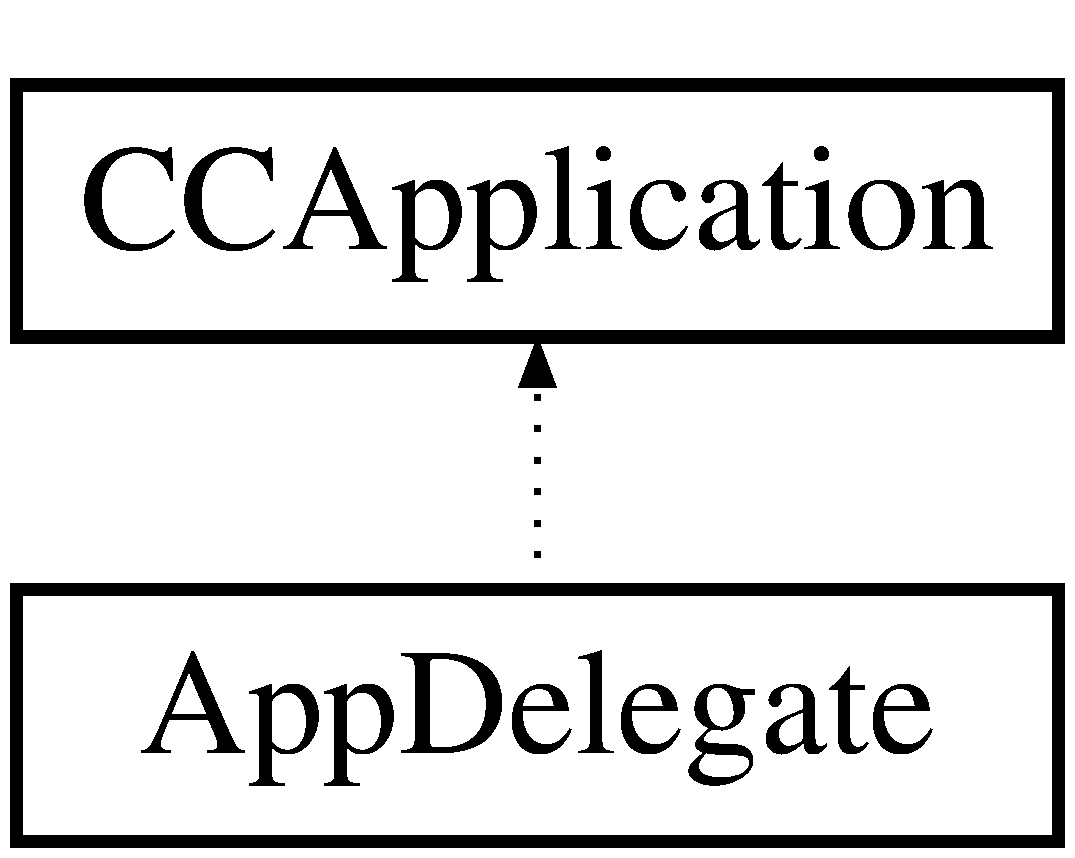
\includegraphics[height=2.000000cm]{class_app_delegate}
\end{center}
\end{figure}
\subsection*{Public Member Functions}
\begin{DoxyCompactItemize}
\item 
virtual bool \hyperlink{class_app_delegate_a68cbaed49edf7581dc59a09d5062fff3}{application\-Did\-Finish\-Launching} ()
\begin{DoxyCompactList}\small\item\em Implement C\-C\-Director and C\-C\-Scene init code here. \end{DoxyCompactList}\item 
virtual void \hyperlink{class_app_delegate_a17cb09777419781698324e0415bffd3a}{application\-Did\-Enter\-Background} ()
\begin{DoxyCompactList}\small\item\em The function be called when the application enter background. \end{DoxyCompactList}\item 
virtual void \hyperlink{class_app_delegate_ac4d653e3f74a91efef5f2def58fe3108}{application\-Will\-Enter\-Foreground} ()
\begin{DoxyCompactList}\small\item\em The function be called when the application enter foreground. \end{DoxyCompactList}\end{DoxyCompactItemize}


\subsection{Member Function Documentation}
\hypertarget{class_app_delegate_a17cb09777419781698324e0415bffd3a}{\index{App\-Delegate@{App\-Delegate}!application\-Did\-Enter\-Background@{application\-Did\-Enter\-Background}}
\index{application\-Did\-Enter\-Background@{application\-Did\-Enter\-Background}!AppDelegate@{App\-Delegate}}
\subsubsection[{application\-Did\-Enter\-Background}]{\setlength{\rightskip}{0pt plus 5cm}void App\-Delegate\-::application\-Did\-Enter\-Background (
\begin{DoxyParamCaption}
{}
\end{DoxyParamCaption}
)\hspace{0.3cm}{\ttfamily [virtual]}}}\label{class_app_delegate_a17cb09777419781698324e0415bffd3a}


The function be called when the application enter background. 


\begin{DoxyParams}{Parameters}
{\em the} & pointer of the application \\
\hline
\end{DoxyParams}
\hypertarget{class_app_delegate_a68cbaed49edf7581dc59a09d5062fff3}{\index{App\-Delegate@{App\-Delegate}!application\-Did\-Finish\-Launching@{application\-Did\-Finish\-Launching}}
\index{application\-Did\-Finish\-Launching@{application\-Did\-Finish\-Launching}!AppDelegate@{App\-Delegate}}
\subsubsection[{application\-Did\-Finish\-Launching}]{\setlength{\rightskip}{0pt plus 5cm}bool App\-Delegate\-::application\-Did\-Finish\-Launching (
\begin{DoxyParamCaption}
{}
\end{DoxyParamCaption}
)\hspace{0.3cm}{\ttfamily [virtual]}}}\label{class_app_delegate_a68cbaed49edf7581dc59a09d5062fff3}


Implement C\-C\-Director and C\-C\-Scene init code here. 

\begin{DoxyReturn}{Returns}
true Initialize success, app continue. 

false Initialize failed, app terminate. 
\end{DoxyReturn}
\hypertarget{class_app_delegate_ac4d653e3f74a91efef5f2def58fe3108}{\index{App\-Delegate@{App\-Delegate}!application\-Will\-Enter\-Foreground@{application\-Will\-Enter\-Foreground}}
\index{application\-Will\-Enter\-Foreground@{application\-Will\-Enter\-Foreground}!AppDelegate@{App\-Delegate}}
\subsubsection[{application\-Will\-Enter\-Foreground}]{\setlength{\rightskip}{0pt plus 5cm}void App\-Delegate\-::application\-Will\-Enter\-Foreground (
\begin{DoxyParamCaption}
{}
\end{DoxyParamCaption}
)\hspace{0.3cm}{\ttfamily [virtual]}}}\label{class_app_delegate_ac4d653e3f74a91efef5f2def58fe3108}


The function be called when the application enter foreground. 


\begin{DoxyParams}{Parameters}
{\em the} & pointer of the application \\
\hline
\end{DoxyParams}


The documentation for this class was generated from the following files\-:\begin{DoxyCompactItemize}
\item 
App\-Delegate.\-h\item 
App\-Delegate.\-cpp\end{DoxyCompactItemize}

\hypertarget{class_j_g___attack_wave___all_lines_sequential}{\section{J\-G\-\_\-\-Attack\-Wave\-\_\-\-All\-Lines\-Sequential Class Reference}
\label{class_j_g___attack_wave___all_lines_sequential}\index{J\-G\-\_\-\-Attack\-Wave\-\_\-\-All\-Lines\-Sequential@{J\-G\-\_\-\-Attack\-Wave\-\_\-\-All\-Lines\-Sequential}}
}
Inheritance diagram for J\-G\-\_\-\-Attack\-Wave\-\_\-\-All\-Lines\-Sequential\-:\begin{figure}[H]
\begin{center}
\leavevmode
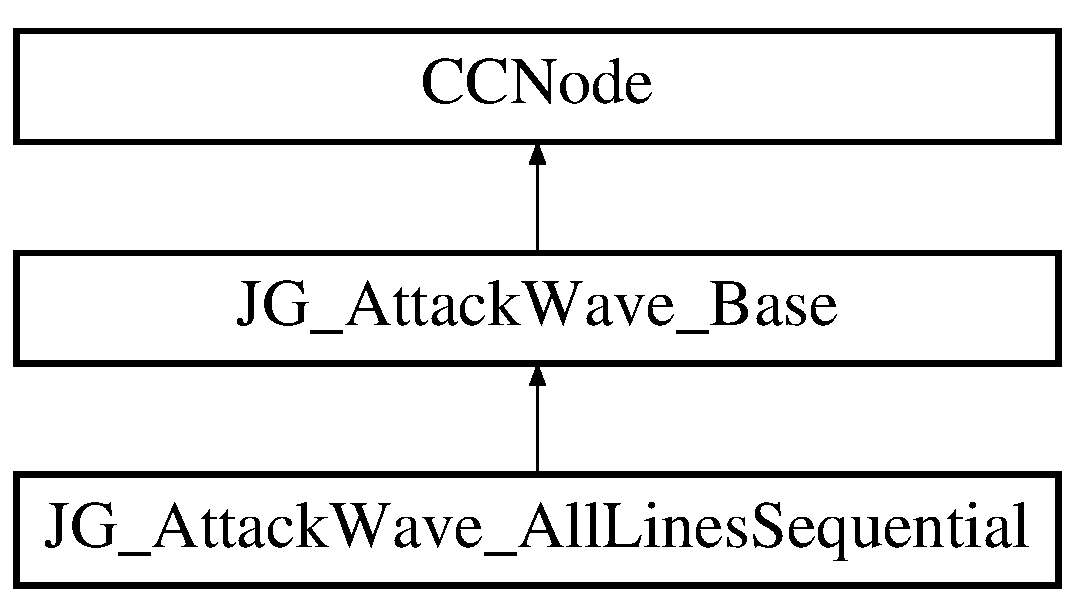
\includegraphics[height=3.000000cm]{class_j_g___attack_wave___all_lines_sequential}
\end{center}
\end{figure}
\subsection*{Public Member Functions}
\begin{DoxyCompactItemize}
\item 
void \hyperlink{class_j_g___attack_wave___all_lines_sequential_afa40aa5942cf470b18e7f41f3e9b2aef}{init\-Attack\-Wave} (float attack\-Difficulty, int attack\-Count)
\item 
\hyperlink{class_j_g___enemy___base}{J\-G\-\_\-\-Enemy\-\_\-\-Base} $\ast$ \hyperlink{class_j_g___attack_wave___all_lines_sequential_a48903ad7c5af66b52df0f5f56d514304}{add\-Enemy} ()
\item 
void \hyperlink{class_j_g___attack_wave___all_lines_sequential_ab5410d3034fee462c0159fbf3685195b}{initiate\-Enemy\-Attack} (float dt)
\item 
float \hyperlink{class_j_g___attack_wave___all_lines_sequential_ab2582130615e79882a153c2572f207c1}{generate\-Enemy\-Position\-Ratio} ()
\item 
void \hyperlink{class_j_g___attack_wave___all_lines_sequential_a597aa5a56da53c430af263cb409c3898}{clalculate\-Enemy\-Add\-Interval} ()
\item 
\hyperlink{class_j_g___path}{J\-G\-\_\-\-Path} $\ast$ \hyperlink{class_j_g___attack_wave___all_lines_sequential_a9220eda05465a8ec13a12b275230c7ed}{select\-Path} (int pathcount)
\item 
\hypertarget{class_j_g___attack_wave___all_lines_sequential_ad500c16193bfbfd3193daa26ab885739}{void {\bfseries update} (float dt)}\label{class_j_g___attack_wave___all_lines_sequential_ad500c16193bfbfd3193daa26ab885739}

\end{DoxyCompactItemize}
\subsection*{Additional Inherited Members}


\subsection{Member Function Documentation}
\hypertarget{class_j_g___attack_wave___all_lines_sequential_a48903ad7c5af66b52df0f5f56d514304}{\index{J\-G\-\_\-\-Attack\-Wave\-\_\-\-All\-Lines\-Sequential@{J\-G\-\_\-\-Attack\-Wave\-\_\-\-All\-Lines\-Sequential}!add\-Enemy@{add\-Enemy}}
\index{add\-Enemy@{add\-Enemy}!JG_AttackWave_AllLinesSequential@{J\-G\-\_\-\-Attack\-Wave\-\_\-\-All\-Lines\-Sequential}}
\subsubsection[{add\-Enemy}]{\setlength{\rightskip}{0pt plus 5cm}{\bf J\-G\-\_\-\-Enemy\-\_\-\-Base} $\ast$ J\-G\-\_\-\-Attack\-Wave\-\_\-\-All\-Lines\-Sequential\-::add\-Enemy (
\begin{DoxyParamCaption}
{}
\end{DoxyParamCaption}
)}}\label{class_j_g___attack_wave___all_lines_sequential_a48903ad7c5af66b52df0f5f56d514304}
Adding a new Enemy \hypertarget{class_j_g___attack_wave___all_lines_sequential_a597aa5a56da53c430af263cb409c3898}{\index{J\-G\-\_\-\-Attack\-Wave\-\_\-\-All\-Lines\-Sequential@{J\-G\-\_\-\-Attack\-Wave\-\_\-\-All\-Lines\-Sequential}!clalculate\-Enemy\-Add\-Interval@{clalculate\-Enemy\-Add\-Interval}}
\index{clalculate\-Enemy\-Add\-Interval@{clalculate\-Enemy\-Add\-Interval}!JG_AttackWave_AllLinesSequential@{J\-G\-\_\-\-Attack\-Wave\-\_\-\-All\-Lines\-Sequential}}
\subsubsection[{clalculate\-Enemy\-Add\-Interval}]{\setlength{\rightskip}{0pt plus 5cm}void J\-G\-\_\-\-Attack\-Wave\-\_\-\-All\-Lines\-Sequential\-::clalculate\-Enemy\-Add\-Interval (
\begin{DoxyParamCaption}
{}
\end{DoxyParamCaption}
)}}\label{class_j_g___attack_wave___all_lines_sequential_a597aa5a56da53c430af263cb409c3898}
Calculating Interval for adding enemy \hypertarget{class_j_g___attack_wave___all_lines_sequential_ab2582130615e79882a153c2572f207c1}{\index{J\-G\-\_\-\-Attack\-Wave\-\_\-\-All\-Lines\-Sequential@{J\-G\-\_\-\-Attack\-Wave\-\_\-\-All\-Lines\-Sequential}!generate\-Enemy\-Position\-Ratio@{generate\-Enemy\-Position\-Ratio}}
\index{generate\-Enemy\-Position\-Ratio@{generate\-Enemy\-Position\-Ratio}!JG_AttackWave_AllLinesSequential@{J\-G\-\_\-\-Attack\-Wave\-\_\-\-All\-Lines\-Sequential}}
\subsubsection[{generate\-Enemy\-Position\-Ratio}]{\setlength{\rightskip}{0pt plus 5cm}float J\-G\-\_\-\-Attack\-Wave\-\_\-\-All\-Lines\-Sequential\-::generate\-Enemy\-Position\-Ratio (
\begin{DoxyParamCaption}
{}
\end{DoxyParamCaption}
)}}\label{class_j_g___attack_wave___all_lines_sequential_ab2582130615e79882a153c2572f207c1}
Generating enemies arriving position \hypertarget{class_j_g___attack_wave___all_lines_sequential_afa40aa5942cf470b18e7f41f3e9b2aef}{\index{J\-G\-\_\-\-Attack\-Wave\-\_\-\-All\-Lines\-Sequential@{J\-G\-\_\-\-Attack\-Wave\-\_\-\-All\-Lines\-Sequential}!init\-Attack\-Wave@{init\-Attack\-Wave}}
\index{init\-Attack\-Wave@{init\-Attack\-Wave}!JG_AttackWave_AllLinesSequential@{J\-G\-\_\-\-Attack\-Wave\-\_\-\-All\-Lines\-Sequential}}
\subsubsection[{init\-Attack\-Wave}]{\setlength{\rightskip}{0pt plus 5cm}void J\-G\-\_\-\-Attack\-Wave\-\_\-\-All\-Lines\-Sequential\-::init\-Attack\-Wave (
\begin{DoxyParamCaption}
\item[{float}]{attack\-Difficulty, }
\item[{int}]{attack\-Count}
\end{DoxyParamCaption}
)\hspace{0.3cm}{\ttfamily [virtual]}}}\label{class_j_g___attack_wave___all_lines_sequential_afa40aa5942cf470b18e7f41f3e9b2aef}
Initializing Attackers wave 

Reimplemented from \hyperlink{class_j_g___attack_wave___base_a5b4110b0837bd6637902c739322a3554}{J\-G\-\_\-\-Attack\-Wave\-\_\-\-Base}.

\hypertarget{class_j_g___attack_wave___all_lines_sequential_ab5410d3034fee462c0159fbf3685195b}{\index{J\-G\-\_\-\-Attack\-Wave\-\_\-\-All\-Lines\-Sequential@{J\-G\-\_\-\-Attack\-Wave\-\_\-\-All\-Lines\-Sequential}!initiate\-Enemy\-Attack@{initiate\-Enemy\-Attack}}
\index{initiate\-Enemy\-Attack@{initiate\-Enemy\-Attack}!JG_AttackWave_AllLinesSequential@{J\-G\-\_\-\-Attack\-Wave\-\_\-\-All\-Lines\-Sequential}}
\subsubsection[{initiate\-Enemy\-Attack}]{\setlength{\rightskip}{0pt plus 5cm}void J\-G\-\_\-\-Attack\-Wave\-\_\-\-All\-Lines\-Sequential\-::initiate\-Enemy\-Attack (
\begin{DoxyParamCaption}
\item[{float}]{dt}
\end{DoxyParamCaption}
)}}\label{class_j_g___attack_wave___all_lines_sequential_ab5410d3034fee462c0159fbf3685195b}
Initializing enemy attack \hypertarget{class_j_g___attack_wave___all_lines_sequential_a9220eda05465a8ec13a12b275230c7ed}{\index{J\-G\-\_\-\-Attack\-Wave\-\_\-\-All\-Lines\-Sequential@{J\-G\-\_\-\-Attack\-Wave\-\_\-\-All\-Lines\-Sequential}!select\-Path@{select\-Path}}
\index{select\-Path@{select\-Path}!JG_AttackWave_AllLinesSequential@{J\-G\-\_\-\-Attack\-Wave\-\_\-\-All\-Lines\-Sequential}}
\subsubsection[{select\-Path}]{\setlength{\rightskip}{0pt plus 5cm}{\bf J\-G\-\_\-\-Path} $\ast$ J\-G\-\_\-\-Attack\-Wave\-\_\-\-All\-Lines\-Sequential\-::select\-Path (
\begin{DoxyParamCaption}
\item[{int}]{pathcount}
\end{DoxyParamCaption}
)}}\label{class_j_g___attack_wave___all_lines_sequential_a9220eda05465a8ec13a12b275230c7ed}
Selecting the sepecified path 

The documentation for this class was generated from the following files\-:\begin{DoxyCompactItemize}
\item 
J\-G\-\_\-\-Attack\-Wave\-\_\-\-All\-Lines\-Sequential.\-h\item 
J\-G\-\_\-\-Attack\-Wave\-\_\-\-All\-Lines\-Sequential.\-cpp\end{DoxyCompactItemize}

\hypertarget{class_j_g___attack_wave___base}{\section{J\-G\-\_\-\-Attack\-Wave\-\_\-\-Base Class Reference}
\label{class_j_g___attack_wave___base}\index{J\-G\-\_\-\-Attack\-Wave\-\_\-\-Base@{J\-G\-\_\-\-Attack\-Wave\-\_\-\-Base}}
}
Inheritance diagram for J\-G\-\_\-\-Attack\-Wave\-\_\-\-Base\-:\begin{figure}[H]
\begin{center}
\leavevmode
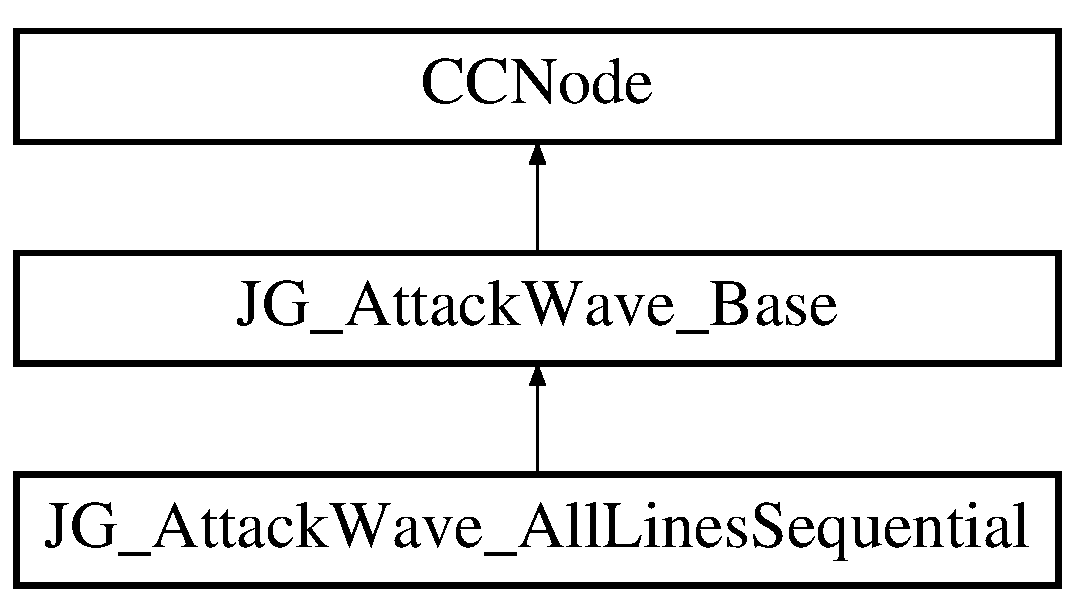
\includegraphics[height=3.000000cm]{class_j_g___attack_wave___base}
\end{center}
\end{figure}
\subsection*{Public Member Functions}
\begin{DoxyCompactItemize}
\item 
int \hyperlink{class_j_g___attack_wave___base_a25af9b766665b528f921daa05f3088f4}{select\-Enemy\-Type} ()
\item 
virtual void \hyperlink{class_j_g___attack_wave___base_a5b4110b0837bd6637902c739322a3554}{init\-Attack\-Wave} (float attack\-Difficulty, int attack\-Count)
\end{DoxyCompactItemize}
\subsection*{Static Public Member Functions}
\begin{DoxyCompactItemize}
\item 
\hypertarget{class_j_g___attack_wave___base_a28fdfe584c2c0a1edaca1a2af26e249d}{static void {\bfseries Set\-Get\-Enemy\-Types\-Function\-Pointer} (C\-C\-Object $\ast$obj, Get\-Enemy\-Types\-Handler)}\label{class_j_g___attack_wave___base_a28fdfe584c2c0a1edaca1a2af26e249d}

\item 
\hypertarget{class_j_g___attack_wave___base_a88332e1e9cc50c5a4fea9597e671265b}{static void {\bfseries Set\-Get\-Balls\-To\-Reward\-Function\-Pointer} (C\-C\-Object $\ast$obj, Get\-Balls\-To\-Reward\-Count\-Handler)}\label{class_j_g___attack_wave___base_a88332e1e9cc50c5a4fea9597e671265b}

\item 
\hypertarget{class_j_g___attack_wave___base_a7bdfecac590df871ea6ebf20e15cfd5e}{static void {\bfseries Set\-Get\-Healthes\-To\-Reward\-Count\-Function\-Pointer} (C\-C\-Object $\ast$obj, Get\-Healthes\-To\-Reward\-Count\-Handler)}\label{class_j_g___attack_wave___base_a7bdfecac590df871ea6ebf20e15cfd5e}

\item 
\hypertarget{class_j_g___attack_wave___base_a8f5501c1c075ca3caefc6ecf658dc30c}{static void {\bfseries Set\-Get\-Pathes\-Array\-Function\-Pointer} (C\-C\-Object $\ast$obj, Get\-Pathes\-Array\-Handler)}\label{class_j_g___attack_wave___base_a8f5501c1c075ca3caefc6ecf658dc30c}

\item 
\hypertarget{class_j_g___attack_wave___base_abd53fbe4eedf618f8e4bd1ffcaae79e7}{static void {\bfseries Set\-On\-Attack\-Wave\-Finished\-Function\-Pointer} (C\-C\-Object $\ast$obj, On\-Attack\-Wave\-Finished\-Handler)}\label{class_j_g___attack_wave___base_abd53fbe4eedf618f8e4bd1ffcaae79e7}

\item 
\hypertarget{class_j_g___attack_wave___base_a2a7e9d8911bc8caec44c0f93694014e6}{static void {\bfseries Set\-On\-Ball\-Rewarded\-Function\-Pointer} (C\-C\-Object $\ast$obj, On\-Ball\-Rewarded\-Handler)}\label{class_j_g___attack_wave___base_a2a7e9d8911bc8caec44c0f93694014e6}

\item 
\hypertarget{class_j_g___attack_wave___base_a8981101a620ac614e91db73449b61a2e}{static void {\bfseries Set\-On\-Health\-Rewarded\-Function\-Pointer} (C\-C\-Object $\ast$obj, On\-Health\-Rewarded\-Handler)}\label{class_j_g___attack_wave___base_a8981101a620ac614e91db73449b61a2e}

\item 
\hypertarget{class_j_g___attack_wave___base_af39c604d6b9eb777d7055d1db90e42d4}{static void {\bfseries Set\-Add\-Enemy\-Function\-Pointer} (C\-C\-Object $\ast$obj, Add\-Enemy\-Handler)}\label{class_j_g___attack_wave___base_af39c604d6b9eb777d7055d1db90e42d4}

\item 
\hypertarget{class_j_g___attack_wave___base_a041bc10cdf5d34df0358118dbfe7e737}{static void {\bfseries Set\-Get\-Available\-Path\-Count\-Function\-Pointer} (C\-C\-Object $\ast$obj, Get\-Available\-Path\-Count\-Handler)}\label{class_j_g___attack_wave___base_a041bc10cdf5d34df0358118dbfe7e737}

\end{DoxyCompactItemize}
\subsection*{Protected Attributes}
\begin{DoxyCompactItemize}
\item 
\hypertarget{class_j_g___attack_wave___base_a12c589b66ecc6b81d2e3ef5b97ab6547}{float {\bfseries attack\-Difficulty}}\label{class_j_g___attack_wave___base_a12c589b66ecc6b81d2e3ef5b97ab6547}

\item 
\hypertarget{class_j_g___attack_wave___base_a4f054cf71992c3d7ea309e49f3e2f27b}{int {\bfseries Get\-Tick\-Count}}\label{class_j_g___attack_wave___base_a4f054cf71992c3d7ea309e49f3e2f27b}

\item 
\hypertarget{class_j_g___attack_wave___base_ab3858590ce216380294c5efaa6ba4fb5}{int {\bfseries attack\-Count}}\label{class_j_g___attack_wave___base_ab3858590ce216380294c5efaa6ba4fb5}

\item 
\hypertarget{class_j_g___attack_wave___base_a3efc437d3866dd40d6b0dc4bb145c468}{int {\bfseries enemy\-Counter}}\label{class_j_g___attack_wave___base_a3efc437d3866dd40d6b0dc4bb145c468}

\end{DoxyCompactItemize}
\subsection*{Static Protected Attributes}
\begin{DoxyCompactItemize}
\item 
\hypertarget{class_j_g___attack_wave___base_ac2fe546212b7cac3526ed7249f3d7faf}{static Get\-Enemy\-Types\-Handler {\bfseries get\-Enemy\-Types\-Function}}\label{class_j_g___attack_wave___base_ac2fe546212b7cac3526ed7249f3d7faf}

\item 
\hypertarget{class_j_g___attack_wave___base_add6c10e9afb81571b060aced881a50c9}{static Get\-Balls\-To\-Reward\-Count\-Handler {\bfseries get\-Balls\-To\-Reward\-Count\-Function}}\label{class_j_g___attack_wave___base_add6c10e9afb81571b060aced881a50c9}

\item 
\hypertarget{class_j_g___attack_wave___base_a3992e58eaab212bf6c40a7d62ba2f780}{static \\*
Get\-Healthes\-To\-Reward\-Count\-Handler {\bfseries get\-Healthes\-To\-Reward\-Count\-Function}}\label{class_j_g___attack_wave___base_a3992e58eaab212bf6c40a7d62ba2f780}

\item 
\hypertarget{class_j_g___attack_wave___base_a83cedf47505a83f7c1a95a7dacbb0c53}{static Get\-Pathes\-Array\-Handler {\bfseries get\-Pathes\-Array\-Function}}\label{class_j_g___attack_wave___base_a83cedf47505a83f7c1a95a7dacbb0c53}

\item 
\hypertarget{class_j_g___attack_wave___base_a8d043885b3b3044a124ca1cb6ff11676}{static On\-Attack\-Wave\-Finished\-Handler {\bfseries on\-Attack\-Wave\-Finished\-Function}}\label{class_j_g___attack_wave___base_a8d043885b3b3044a124ca1cb6ff11676}

\item 
\hypertarget{class_j_g___attack_wave___base_afa6edd2b0d2d6ad40f5c64c9dd2271b2}{static On\-Health\-Rewarded\-Handler {\bfseries on\-Health\-Rewarded\-Function}}\label{class_j_g___attack_wave___base_afa6edd2b0d2d6ad40f5c64c9dd2271b2}

\item 
\hypertarget{class_j_g___attack_wave___base_a64fbfb8d3a8710b08a261c97116dd05d}{static On\-Ball\-Rewarded\-Handler {\bfseries on\-Ball\-Rewarded\-Function}}\label{class_j_g___attack_wave___base_a64fbfb8d3a8710b08a261c97116dd05d}

\item 
\hypertarget{class_j_g___attack_wave___base_ac93b8e2206fe78ce985d4424ba2e9ace}{static Add\-Enemy\-Handler {\bfseries add\-Enemy\-Function}}\label{class_j_g___attack_wave___base_ac93b8e2206fe78ce985d4424ba2e9ace}

\item 
\hypertarget{class_j_g___attack_wave___base_a5f6dee9c5f856be1188e2b750e2fe133}{static Get\-Available\-Path\-Count\-Handler {\bfseries get\-Available\-Path\-Count\-Function}}\label{class_j_g___attack_wave___base_a5f6dee9c5f856be1188e2b750e2fe133}

\item 
\hypertarget{class_j_g___attack_wave___base_aade81a1ff1cdb44768637cec2291b769}{static C\-C\-Object $\ast$ {\bfseries listener\-Obj}}\label{class_j_g___attack_wave___base_aade81a1ff1cdb44768637cec2291b769}

\end{DoxyCompactItemize}


\subsection{Member Function Documentation}
\hypertarget{class_j_g___attack_wave___base_a5b4110b0837bd6637902c739322a3554}{\index{J\-G\-\_\-\-Attack\-Wave\-\_\-\-Base@{J\-G\-\_\-\-Attack\-Wave\-\_\-\-Base}!init\-Attack\-Wave@{init\-Attack\-Wave}}
\index{init\-Attack\-Wave@{init\-Attack\-Wave}!JG_AttackWave_Base@{J\-G\-\_\-\-Attack\-Wave\-\_\-\-Base}}
\subsubsection[{init\-Attack\-Wave}]{\setlength{\rightskip}{0pt plus 5cm}void J\-G\-\_\-\-Attack\-Wave\-\_\-\-Base\-::init\-Attack\-Wave (
\begin{DoxyParamCaption}
\item[{float}]{attack\-Difficulty, }
\item[{int}]{attack\-Count}
\end{DoxyParamCaption}
)\hspace{0.3cm}{\ttfamily [virtual]}}}\label{class_j_g___attack_wave___base_a5b4110b0837bd6637902c739322a3554}
Initializing Attack Wave 

Reimplemented in \hyperlink{class_j_g___attack_wave___all_lines_sequential_afa40aa5942cf470b18e7f41f3e9b2aef}{J\-G\-\_\-\-Attack\-Wave\-\_\-\-All\-Lines\-Sequential}.

\hypertarget{class_j_g___attack_wave___base_a25af9b766665b528f921daa05f3088f4}{\index{J\-G\-\_\-\-Attack\-Wave\-\_\-\-Base@{J\-G\-\_\-\-Attack\-Wave\-\_\-\-Base}!select\-Enemy\-Type@{select\-Enemy\-Type}}
\index{select\-Enemy\-Type@{select\-Enemy\-Type}!JG_AttackWave_Base@{J\-G\-\_\-\-Attack\-Wave\-\_\-\-Base}}
\subsubsection[{select\-Enemy\-Type}]{\setlength{\rightskip}{0pt plus 5cm}int J\-G\-\_\-\-Attack\-Wave\-\_\-\-Base\-::select\-Enemy\-Type (
\begin{DoxyParamCaption}
{}
\end{DoxyParamCaption}
)}}\label{class_j_g___attack_wave___base_a25af9b766665b528f921daa05f3088f4}
Selecting Type of the Enemy 

The documentation for this class was generated from the following files\-:\begin{DoxyCompactItemize}
\item 
J\-G\-\_\-\-Attack\-Wave\-\_\-\-Base.\-h\item 
J\-G\-\_\-\-Attack\-Wave\-\_\-\-Base.\-cpp\end{DoxyCompactItemize}

\hypertarget{class_j_g___ball}{\section{J\-G\-\_\-\-Ball Class Reference}
\label{class_j_g___ball}\index{J\-G\-\_\-\-Ball@{J\-G\-\_\-\-Ball}}
}


{\ttfamily \#include $<$J\-G\-\_\-\-Ball.\-h$>$}

Inheritance diagram for J\-G\-\_\-\-Ball\-:\begin{figure}[H]
\begin{center}
\leavevmode
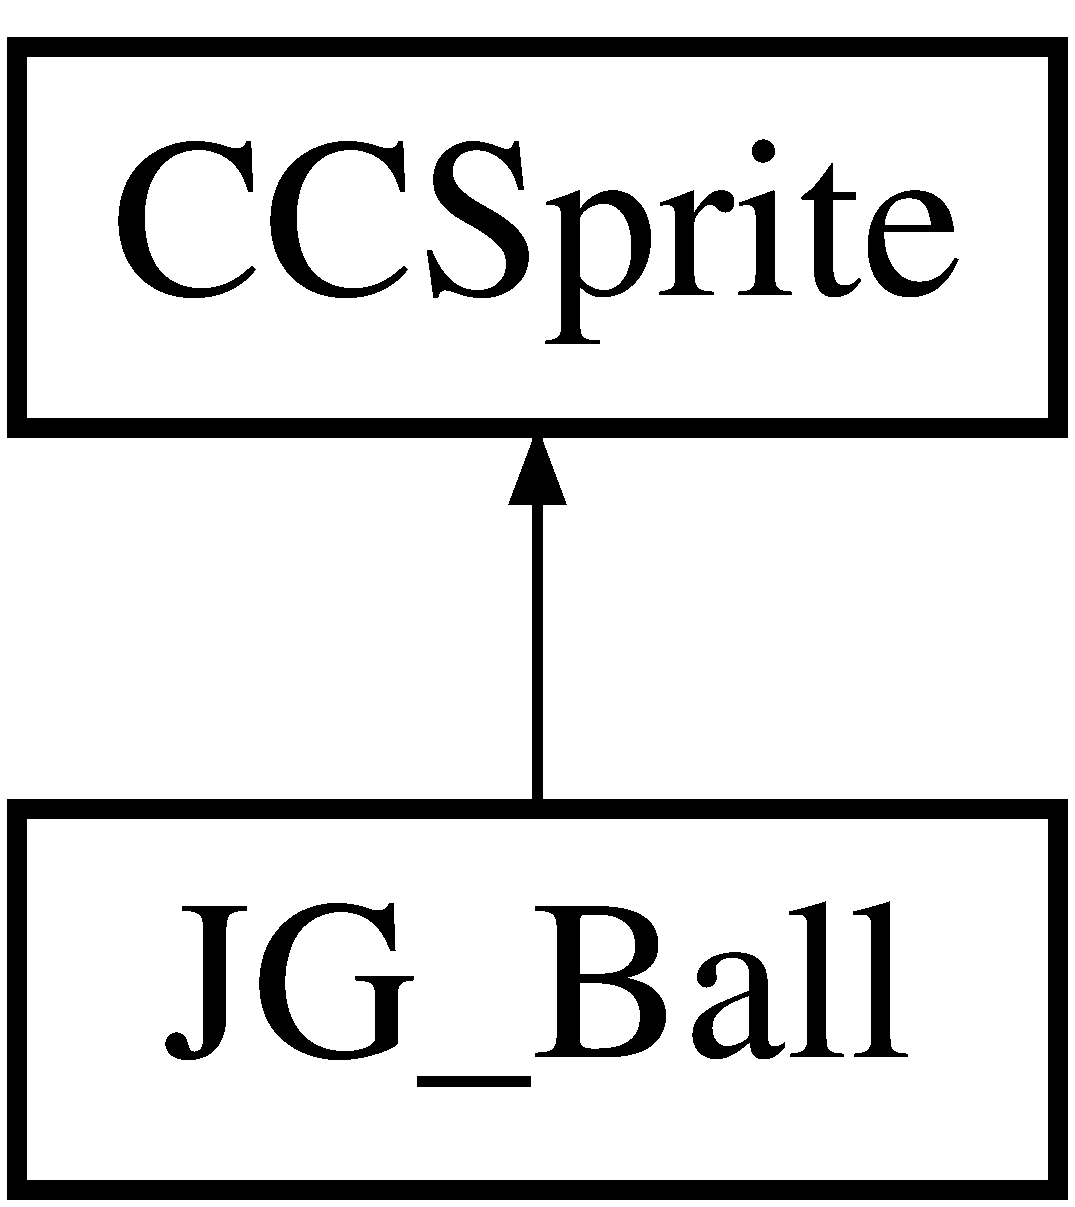
\includegraphics[height=2.000000cm]{class_j_g___ball}
\end{center}
\end{figure}
\subsection*{Public Member Functions}
\begin{DoxyCompactItemize}
\item 
void \hyperlink{class_j_g___ball_a601eda0b1aaf9d4c8fdd31d36234a6c1}{Move\-Curve} (float force, C\-C\-Point destination)
\item 
void \hyperlink{class_j_g___ball_afa347dae4a20695cf506375b798cb2f3}{Move\-Staight} (float force, C\-C\-Point destination)
\item 
void \hyperlink{class_j_g___ball_a21c06d1a10aa8fdcc3d8e63a82f221fe}{update} (float dt)
\item 
\hypertarget{class_j_g___ball_adb4350ed0da24e5499c3402bc322f559}{void {\bfseries temp\-Reset} ()}\label{class_j_g___ball_adb4350ed0da24e5499c3402bc322f559}

\item 
E\-Throw\-Direction \hyperlink{class_j_g___ball_a94843b91ab6f8cddbb2b90de6daeb531}{Get\-Ball\-Direction} ()
\item 
\hypertarget{class_j_g___ball_a0ad42506b43718f14ccb45f163d92999}{C\-C\-Point {\bfseries Get\-Initial\-Touch\-Position} ()}\label{class_j_g___ball_a0ad42506b43718f14ccb45f163d92999}

\item 
\hypertarget{class_j_g___ball_a628e6f457315f1af9d9638834dff91e0}{void {\bfseries Set\-Initial\-Touch\-Position} (C\-C\-Point new\-Touch\-Pos)}\label{class_j_g___ball_a628e6f457315f1af9d9638834dff91e0}

\end{DoxyCompactItemize}
\subsection*{Static Public Member Functions}
\begin{DoxyCompactItemize}
\item 
static \hyperlink{class_j_g___ball}{J\-G\-\_\-\-Ball} $\ast$ \hyperlink{class_j_g___ball_a12279a500446c9516026d3f52fee87eb}{create\-With\-File\-Name} (const char $\ast$psz\-File\-Name, C\-C\-Point initial\-Pos)
\item 
static void \hyperlink{class_j_g___ball_a8023f3c38c257dd4430a5a01c519a289}{Calculate\-Speed\-Boundries\-Base\-On\-Length} (float delta\-X)
\end{DoxyCompactItemize}
\subsection*{Public Attributes}
\begin{DoxyCompactItemize}
\item 
\hypertarget{class_j_g___ball_ad4aa2855022e5315addf40ef73ee6972}{float {\bfseries speed}}\label{class_j_g___ball_ad4aa2855022e5315addf40ef73ee6972}

\item 
\hypertarget{class_j_g___ball_a743ed73473f38e9466f305c3f8efe995}{E\-Throw\-Direction {\bfseries ball\-Throw\-Direction}}\label{class_j_g___ball_a743ed73473f38e9466f305c3f8efe995}

\item 
\hypertarget{class_j_g___ball_af0bd7eeacc5d8f094d921663843b5179}{float {\bfseries curve\-\_\-\-Total\-Time}}\label{class_j_g___ball_af0bd7eeacc5d8f094d921663843b5179}

\item 
\hypertarget{class_j_g___ball_a681ecc9587d2d8d857f656d19d297ef8}{float {\bfseries curve\-\_\-\-Y0}}\label{class_j_g___ball_a681ecc9587d2d8d857f656d19d297ef8}

\item 
\hypertarget{class_j_g___ball_a8dcbff9b6d7f9f8737b3421f26c699e7}{float {\bfseries curve\-\_\-\-X0}}\label{class_j_g___ball_a8dcbff9b6d7f9f8737b3421f26c699e7}

\item 
\hypertarget{class_j_g___ball_a32222cd24992fff289361884db472b23}{float {\bfseries curve\-\_\-\-Rad}}\label{class_j_g___ball_a32222cd24992fff289361884db472b23}

\item 
\hypertarget{class_j_g___ball_a399ae1fb026df3759d3616c7b74eecaa}{float {\bfseries straight\-\_\-\-Dir}}\label{class_j_g___ball_a399ae1fb026df3759d3616c7b74eecaa}

\item 
\hypertarget{class_j_g___ball_a2cab0645b2eb4374fbfde0b0399c0e72}{C\-C\-Point {\bfseries temp\-Initial\-Position}}\label{class_j_g___ball_a2cab0645b2eb4374fbfde0b0399c0e72}

\item 
\hypertarget{class_j_g___ball_a358259dea815fa262327e0af48a6af3c}{E\-Throw\-Direction {\bfseries temp\-Initial\-Throw\-Direction}}\label{class_j_g___ball_a358259dea815fa262327e0af48a6af3c}

\item 
\hypertarget{class_j_g___ball_a602558390080ce6d8cdfcfdbc09f7b12}{C\-C\-Repeat\-Forever $\ast$ {\bfseries action\-\_\-\-Rotate}}\label{class_j_g___ball_a602558390080ce6d8cdfcfdbc09f7b12}

\item 
\hypertarget{class_j_g___ball_aa0fc27312d724fcf2324e87844a99cb8}{\hyperlink{class_j_g___temp_line_container}{J\-G\-\_\-\-Temp\-Line\-Container} $\ast$ {\bfseries temp\-Draw}}\label{class_j_g___ball_aa0fc27312d724fcf2324e87844a99cb8}

\item 
\hypertarget{class_j_g___ball_aacc0e044d12a3fe88d03b54f8c800626}{C\-C\-Point {\bfseries touch\-Position}}\label{class_j_g___ball_aacc0e044d12a3fe88d03b54f8c800626}

\item 
\hypertarget{class_j_g___ball_a0ad0f2f4b8d03d63c879544111a24506}{E\-Move\-Mode {\bfseries move\-Mode}}\label{class_j_g___ball_a0ad0f2f4b8d03d63c879544111a24506}

\end{DoxyCompactItemize}
\subsection*{Static Public Attributes}
\begin{DoxyCompactItemize}
\item 
\hypertarget{class_j_g___ball_a0e5845ccdb93030b567b796f6266e517}{static float {\bfseries min\-Speed}}\label{class_j_g___ball_a0e5845ccdb93030b567b796f6266e517}

\item 
\hypertarget{class_j_g___ball_ad830251662cdf8443962aef638ffefcc}{static float {\bfseries max\-Speed}}\label{class_j_g___ball_ad830251662cdf8443962aef638ffefcc}

\end{DoxyCompactItemize}


\subsection{Detailed Description}
class for handling ball 

\subsection{Member Function Documentation}
\hypertarget{class_j_g___ball_a8023f3c38c257dd4430a5a01c519a289}{\index{J\-G\-\_\-\-Ball@{J\-G\-\_\-\-Ball}!Calculate\-Speed\-Boundries\-Base\-On\-Length@{Calculate\-Speed\-Boundries\-Base\-On\-Length}}
\index{Calculate\-Speed\-Boundries\-Base\-On\-Length@{Calculate\-Speed\-Boundries\-Base\-On\-Length}!JG_Ball@{J\-G\-\_\-\-Ball}}
\subsubsection[{Calculate\-Speed\-Boundries\-Base\-On\-Length}]{\setlength{\rightskip}{0pt plus 5cm}static void J\-G\-\_\-\-Ball\-::\-Calculate\-Speed\-Boundries\-Base\-On\-Length (
\begin{DoxyParamCaption}
\item[{float}]{delta\-X}
\end{DoxyParamCaption}
)\hspace{0.3cm}{\ttfamily [inline]}, {\ttfamily [static]}}}\label{class_j_g___ball_a8023f3c38c257dd4430a5a01c519a289}
Calculate the minimum Speed , based on the distance of handes \hypertarget{class_j_g___ball_a12279a500446c9516026d3f52fee87eb}{\index{J\-G\-\_\-\-Ball@{J\-G\-\_\-\-Ball}!create\-With\-File\-Name@{create\-With\-File\-Name}}
\index{create\-With\-File\-Name@{create\-With\-File\-Name}!JG_Ball@{J\-G\-\_\-\-Ball}}
\subsubsection[{create\-With\-File\-Name}]{\setlength{\rightskip}{0pt plus 5cm}{\bf J\-G\-\_\-\-Ball} $\ast$ J\-G\-\_\-\-Ball\-::create\-With\-File\-Name (
\begin{DoxyParamCaption}
\item[{const char $\ast$}]{psz\-File\-Name, }
\item[{C\-C\-Point}]{initial\-Pos}
\end{DoxyParamCaption}
)\hspace{0.3cm}{\ttfamily [static]}}}\label{class_j_g___ball_a12279a500446c9516026d3f52fee87eb}
Creating ball in a specific position \hypertarget{class_j_g___ball_a94843b91ab6f8cddbb2b90de6daeb531}{\index{J\-G\-\_\-\-Ball@{J\-G\-\_\-\-Ball}!Get\-Ball\-Direction@{Get\-Ball\-Direction}}
\index{Get\-Ball\-Direction@{Get\-Ball\-Direction}!JG_Ball@{J\-G\-\_\-\-Ball}}
\subsubsection[{Get\-Ball\-Direction}]{\setlength{\rightskip}{0pt plus 5cm}E\-Throw\-Direction J\-G\-\_\-\-Ball\-::\-Get\-Ball\-Direction (
\begin{DoxyParamCaption}
{}
\end{DoxyParamCaption}
)\hspace{0.3cm}{\ttfamily [inline]}}}\label{class_j_g___ball_a94843b91ab6f8cddbb2b90de6daeb531}
get the direction of ball \hypertarget{class_j_g___ball_a601eda0b1aaf9d4c8fdd31d36234a6c1}{\index{J\-G\-\_\-\-Ball@{J\-G\-\_\-\-Ball}!Move\-Curve@{Move\-Curve}}
\index{Move\-Curve@{Move\-Curve}!JG_Ball@{J\-G\-\_\-\-Ball}}
\subsubsection[{Move\-Curve}]{\setlength{\rightskip}{0pt plus 5cm}void J\-G\-\_\-\-Ball\-::\-Move\-Curve (
\begin{DoxyParamCaption}
\item[{float}]{force, }
\item[{C\-C\-Point}]{destination}
\end{DoxyParamCaption}
)}}\label{class_j_g___ball_a601eda0b1aaf9d4c8fdd31d36234a6c1}
Initial the curve movement variables \hypertarget{class_j_g___ball_afa347dae4a20695cf506375b798cb2f3}{\index{J\-G\-\_\-\-Ball@{J\-G\-\_\-\-Ball}!Move\-Staight@{Move\-Staight}}
\index{Move\-Staight@{Move\-Staight}!JG_Ball@{J\-G\-\_\-\-Ball}}
\subsubsection[{Move\-Staight}]{\setlength{\rightskip}{0pt plus 5cm}void J\-G\-\_\-\-Ball\-::\-Move\-Staight (
\begin{DoxyParamCaption}
\item[{float}]{force, }
\item[{C\-C\-Point}]{destination}
\end{DoxyParamCaption}
)}}\label{class_j_g___ball_afa347dae4a20695cf506375b798cb2f3}
Initial the straight movement variables \hypertarget{class_j_g___ball_a21c06d1a10aa8fdcc3d8e63a82f221fe}{\index{J\-G\-\_\-\-Ball@{J\-G\-\_\-\-Ball}!update@{update}}
\index{update@{update}!JG_Ball@{J\-G\-\_\-\-Ball}}
\subsubsection[{update}]{\setlength{\rightskip}{0pt plus 5cm}void J\-G\-\_\-\-Ball\-::update (
\begin{DoxyParamCaption}
\item[{float}]{dt}
\end{DoxyParamCaption}
)}}\label{class_j_g___ball_a21c06d1a10aa8fdcc3d8e63a82f221fe}
Handles the movement based on the current mode 

The documentation for this class was generated from the following files\-:\begin{DoxyCompactItemize}
\item 
J\-G\-\_\-\-Ball.\-h\item 
J\-G\-\_\-\-Ball.\-cpp\end{DoxyCompactItemize}

\hypertarget{class_j_g___bonus___base}{\section{J\-G\-\_\-\-Bonus\-\_\-\-Base Class Reference}
\label{class_j_g___bonus___base}\index{J\-G\-\_\-\-Bonus\-\_\-\-Base@{J\-G\-\_\-\-Bonus\-\_\-\-Base}}
}
Inheritance diagram for J\-G\-\_\-\-Bonus\-\_\-\-Base\-:\begin{figure}[H]
\begin{center}
\leavevmode
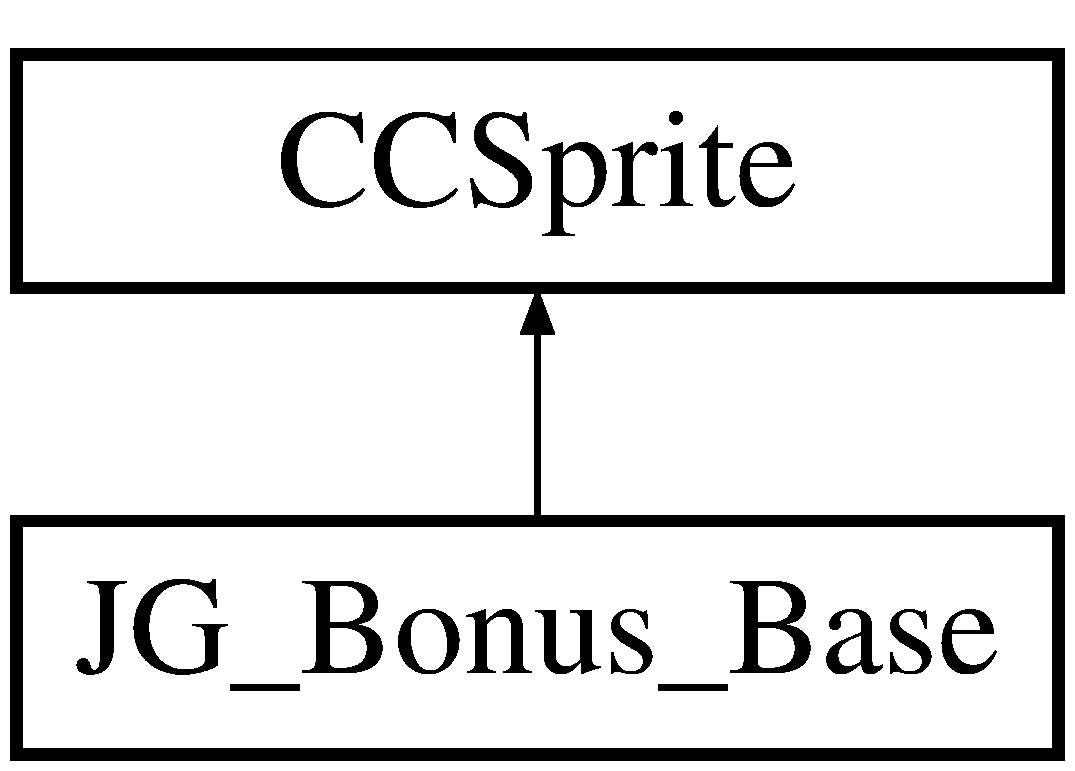
\includegraphics[height=2.000000cm]{class_j_g___bonus___base}
\end{center}
\end{figure}


The documentation for this class was generated from the following files\-:\begin{DoxyCompactItemize}
\item 
J\-G\-\_\-\-Bonus\-\_\-\-Base.\-h\item 
J\-G\-\_\-\-Bonus\-\_\-\-Base.\-cpp\end{DoxyCompactItemize}

\hypertarget{class_j_g___enemy___base}{\section{J\-G\-\_\-\-Enemy\-\_\-\-Base Class Reference}
\label{class_j_g___enemy___base}\index{J\-G\-\_\-\-Enemy\-\_\-\-Base@{J\-G\-\_\-\-Enemy\-\_\-\-Base}}
}
Inheritance diagram for J\-G\-\_\-\-Enemy\-\_\-\-Base\-:\begin{figure}[H]
\begin{center}
\leavevmode
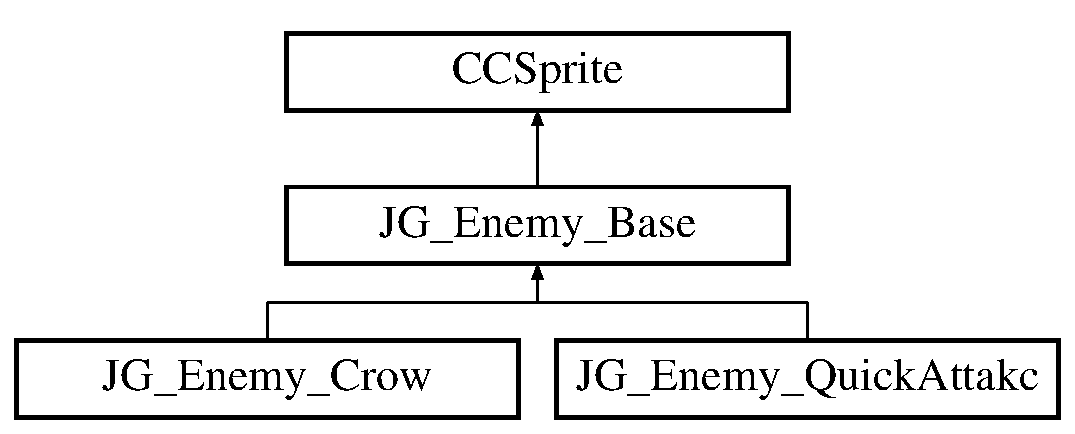
\includegraphics[height=3.000000cm]{class_j_g___enemy___base}
\end{center}
\end{figure}
\subsection*{Public Member Functions}
\begin{DoxyCompactItemize}
\item 
void \hyperlink{class_j_g___enemy___base_a0c32f5ce5ebd4d988ca7f2eb485634c5}{Move\-To} (float dt)
\item 
void \hyperlink{class_j_g___enemy___base_a9ec36f3012a3bc79f5f4da1efd0f5a17}{Set\-Destination\-Path} (C\-C\-Point destination\-Pos, \hyperlink{class_j_g___path}{J\-G\-\_\-\-Path} $\ast$new\-Target\-Path)
\item 
void \hyperlink{class_j_g___enemy___base_a44b421c3ab84dce24b4c59f3c5d94c5c}{Set\-Destination\-Position} (C\-C\-Point destinaion\-Pos)
\item 
void \hyperlink{class_j_g___enemy___base_a981f54e4d7f7fb1e10e57ce5ae0e7e6c}{Check\-Out\-Of\-Screen} ()
\item 
void \hyperlink{class_j_g___enemy___base_af7d600c7327aa775fc3149b76b8d7050}{Set\-State} (E\-Enemy\-State state)
\item 
void \hyperlink{class_j_g___enemy___base_ae7d83ddaed626a47dda3d14c26c94f44}{Fall} (float dt)
\item 
virtual void \hyperlink{class_j_g___enemy___base_a8dacf683f1b41612faf87df7f144cf81}{Initial\-Enemy} (C\-C\-Point initial\-Position)
\item 
virtual void \hyperlink{class_j_g___enemy___base_acdfcfb221314eb5c3067aacb8aa4d34f}{Initial\-Enemy} (C\-C\-Point initial\-Position, E\-Enemy\-Bonus bonus)
\item 
void \hyperlink{class_j_g___enemy___base_a026d475d28ed59d88c00d55622ffb501}{update} (float dt)
\item 
void \hyperlink{class_j_g___enemy___base_a7b292e23ac507fe700721cbfb363c5ab}{Check\-Collision\-With\-Ball} ()
\item 
void \hyperlink{class_j_g___enemy___base_aa3a97d79f8845764a9934696b4ab5303}{Process\-Move} (float dt)
\item 
void \hyperlink{class_j_g___enemy___base_a78e893ce15f84acd45b310d1d7f2d62c}{Handle\-Waiting\-To\-Attacking} (float time)
\item 
void \hyperlink{class_j_g___enemy___base_ab502e8bfc62c219a5a53fa64f73ceace}{Initial\-Intending\-Animation} ()
\item 
void \hyperlink{class_j_g___enemy___base_a04f490f8d7d07bddba76ab7dd7dcc2a4}{Initial\-Attacking\-Animation} ()
\item 
void \hyperlink{class_j_g___enemy___base_addc7dc8e7ee789b629a442b63a61f205}{Initial\-Waiting\-Animation} ()
\item 
void \hyperlink{class_j_g___enemy___base_a6dd7be9c41d58787a6bb2b461b4fa343}{Initial\-Escaping\-Animation} ()
\item 
void \hyperlink{class_j_g___enemy___base_a793996b953546bd76ab1483e8d62ed65}{Initial\-Dying\-Animation} ()
\item 
void \hyperlink{class_j_g___enemy___base_a6754c7a2a6fc9f2877f57c6a868706d8}{Run\-Animation} (C\-C\-Animation $\ast$animation)
\item 
void \hyperlink{class_j_g___enemy___base_a4ab46247bd7d721286c3196f8fcdbf3a}{draw} ()
\item 
E\-Enemy\-Bonus \hyperlink{class_j_g___enemy___base_af71160543647fad96886e1f87b580896}{Get\-Enemy\-Bonus} ()
\item 
float \hyperlink{class_j_g___enemy___base_a3b1c2a3166cd9dbd3aefc79542f36d16}{Get\-Difficulty} ()
\item 
\hyperlink{class_j_g___path}{J\-G\-\_\-\-Path} $\ast$ \hyperlink{class_j_g___enemy___base_a8ce8d53876f32eea86ed76d6448d5791}{Get\-Target\-Path} ()
\item 
void \hyperlink{class_j_g___enemy___base_afd08277de6792e48a0c33edaada7ca42}{Set\-Enemy\-Bonus} (E\-Enemy\-Bonus bonus)
\end{DoxyCompactItemize}
\subsection*{Static Public Member Functions}
\begin{DoxyCompactItemize}
\item 
\hypertarget{class_j_g___enemy___base_aa9057195c83084f43facd26cd26c2bcc}{static void {\bfseries Set\-On\-Lost\-Function\-Pointer} (C\-C\-Object $\ast$rec, On\-Lost\-Handler)}\label{class_j_g___enemy___base_aa9057195c83084f43facd26cd26c2bcc}

\item 
\hypertarget{class_j_g___enemy___base_ac3fa895795c80fa6b5213bdb136bcb83}{static void {\bfseries Set\-On\-Hit\-Function\-Pointer} (C\-C\-Object $\ast$rec, On\-Hit\-Handler)}\label{class_j_g___enemy___base_ac3fa895795c80fa6b5213bdb136bcb83}

\item 
\hypertarget{class_j_g___enemy___base_a1e3731cde597d162b35e2df1a57bbd45}{static void {\bfseries Set\-Get\-Balls\-Function\-Pointer} (C\-C\-Object $\ast$obj, Get\-Balls\-Handler)}\label{class_j_g___enemy___base_a1e3731cde597d162b35e2df1a57bbd45}

\item 
\hypertarget{class_j_g___enemy___base_a6df960380bf013523c12062d91227bcd}{static void {\bfseries Set\-Damage\-Path\-Function\-Pointer} (C\-C\-Object $\ast$obj, Damage\-Path\-Handler)}\label{class_j_g___enemy___base_a6df960380bf013523c12062d91227bcd}

\item 
static \hyperlink{class_j_g___enemy___base}{J\-G\-\_\-\-Enemy\-\_\-\-Base} $\ast$ \hyperlink{class_j_g___enemy___base_a928a5124a9a1dbf000c7b1d6b357b960}{Create\-Enemy} (C\-C\-Point initial\-Position)
\end{DoxyCompactItemize}
\subsection*{Public Attributes}
\begin{DoxyCompactItemize}
\item 
C\-C\-Animation $\ast$ \hyperlink{class_j_g___enemy___base_abbee7e77ffc238b8ce725bf749d771a7}{intending\-Animation}
\item 
\hypertarget{class_j_g___enemy___base_aba40ca3bfdf2755f1e54d839765e3dc7}{C\-C\-Animation $\ast$ {\bfseries attacking\-Animation}}\label{class_j_g___enemy___base_aba40ca3bfdf2755f1e54d839765e3dc7}

\item 
\hypertarget{class_j_g___enemy___base_a717c32a58a7d762f041613d75693a4c4}{C\-C\-Animation $\ast$ {\bfseries waiting\-Animation}}\label{class_j_g___enemy___base_a717c32a58a7d762f041613d75693a4c4}

\item 
\hypertarget{class_j_g___enemy___base_a6a021809fe18be6659ec986a6566658a}{C\-C\-Animation $\ast$ {\bfseries escaping\-Animation}}\label{class_j_g___enemy___base_a6a021809fe18be6659ec986a6566658a}

\item 
\hypertarget{class_j_g___enemy___base_a2a6b96de6f7d97b9bf6bf92fbdd0555f}{C\-C\-Animation $\ast$ {\bfseries dying\-Animation}}\label{class_j_g___enemy___base_a2a6b96de6f7d97b9bf6bf92fbdd0555f}

\item 
\hypertarget{class_j_g___enemy___base_a7d27718a30d366cf8934c85c423c57fc}{C\-C\-Animate $\ast$ {\bfseries animation\-Action}}\label{class_j_g___enemy___base_a7d27718a30d366cf8934c85c423c57fc}

\item 
\hypertarget{class_j_g___enemy___base_a433673314d91e149ab333347e9cc046d}{C\-C\-Texture2\-D $\ast$ {\bfseries ball\-Bonus\-Texture}}\label{class_j_g___enemy___base_a433673314d91e149ab333347e9cc046d}

\item 
\hypertarget{class_j_g___enemy___base_a3e59ea611043e0bfb426e4391cc070e7}{C\-C\-String {\bfseries sprite\-File\-Name}}\label{class_j_g___enemy___base_a3e59ea611043e0bfb426e4391cc070e7}

\end{DoxyCompactItemize}


\subsection{Member Function Documentation}
\hypertarget{class_j_g___enemy___base_a7b292e23ac507fe700721cbfb363c5ab}{\index{J\-G\-\_\-\-Enemy\-\_\-\-Base@{J\-G\-\_\-\-Enemy\-\_\-\-Base}!Check\-Collision\-With\-Ball@{Check\-Collision\-With\-Ball}}
\index{Check\-Collision\-With\-Ball@{Check\-Collision\-With\-Ball}!JG_Enemy_Base@{J\-G\-\_\-\-Enemy\-\_\-\-Base}}
\subsubsection[{Check\-Collision\-With\-Ball}]{\setlength{\rightskip}{0pt plus 5cm}void J\-G\-\_\-\-Enemy\-\_\-\-Base\-::\-Check\-Collision\-With\-Ball (
\begin{DoxyParamCaption}
{}
\end{DoxyParamCaption}
)}}\label{class_j_g___enemy___base_a7b292e23ac507fe700721cbfb363c5ab}
Checking enemy collision with ball \hypertarget{class_j_g___enemy___base_a981f54e4d7f7fb1e10e57ce5ae0e7e6c}{\index{J\-G\-\_\-\-Enemy\-\_\-\-Base@{J\-G\-\_\-\-Enemy\-\_\-\-Base}!Check\-Out\-Of\-Screen@{Check\-Out\-Of\-Screen}}
\index{Check\-Out\-Of\-Screen@{Check\-Out\-Of\-Screen}!JG_Enemy_Base@{J\-G\-\_\-\-Enemy\-\_\-\-Base}}
\subsubsection[{Check\-Out\-Of\-Screen}]{\setlength{\rightskip}{0pt plus 5cm}void J\-G\-\_\-\-Enemy\-\_\-\-Base\-::\-Check\-Out\-Of\-Screen (
\begin{DoxyParamCaption}
{}
\end{DoxyParamCaption}
)}}\label{class_j_g___enemy___base_a981f54e4d7f7fb1e10e57ce5ae0e7e6c}
To check if the Enemy is out the screen \hypertarget{class_j_g___enemy___base_a928a5124a9a1dbf000c7b1d6b357b960}{\index{J\-G\-\_\-\-Enemy\-\_\-\-Base@{J\-G\-\_\-\-Enemy\-\_\-\-Base}!Create\-Enemy@{Create\-Enemy}}
\index{Create\-Enemy@{Create\-Enemy}!JG_Enemy_Base@{J\-G\-\_\-\-Enemy\-\_\-\-Base}}
\subsubsection[{Create\-Enemy}]{\setlength{\rightskip}{0pt plus 5cm}{\bf J\-G\-\_\-\-Enemy\-\_\-\-Base} $\ast$ J\-G\-\_\-\-Enemy\-\_\-\-Base\-::\-Create\-Enemy (
\begin{DoxyParamCaption}
\item[{C\-C\-Point}]{initial\-Position}
\end{DoxyParamCaption}
)\hspace{0.3cm}{\ttfamily [static]}}}\label{class_j_g___enemy___base_a928a5124a9a1dbf000c7b1d6b357b960}
Creating the new enemy \hypertarget{class_j_g___enemy___base_a4ab46247bd7d721286c3196f8fcdbf3a}{\index{J\-G\-\_\-\-Enemy\-\_\-\-Base@{J\-G\-\_\-\-Enemy\-\_\-\-Base}!draw@{draw}}
\index{draw@{draw}!JG_Enemy_Base@{J\-G\-\_\-\-Enemy\-\_\-\-Base}}
\subsubsection[{draw}]{\setlength{\rightskip}{0pt plus 5cm}void J\-G\-\_\-\-Enemy\-\_\-\-Base\-::draw (
\begin{DoxyParamCaption}
{}
\end{DoxyParamCaption}
)}}\label{class_j_g___enemy___base_a4ab46247bd7d721286c3196f8fcdbf3a}
Draw the sprite \hypertarget{class_j_g___enemy___base_ae7d83ddaed626a47dda3d14c26c94f44}{\index{J\-G\-\_\-\-Enemy\-\_\-\-Base@{J\-G\-\_\-\-Enemy\-\_\-\-Base}!Fall@{Fall}}
\index{Fall@{Fall}!JG_Enemy_Base@{J\-G\-\_\-\-Enemy\-\_\-\-Base}}
\subsubsection[{Fall}]{\setlength{\rightskip}{0pt plus 5cm}void J\-G\-\_\-\-Enemy\-\_\-\-Base\-::\-Fall (
\begin{DoxyParamCaption}
\item[{float}]{dt}
\end{DoxyParamCaption}
)}}\label{class_j_g___enemy___base_ae7d83ddaed626a47dda3d14c26c94f44}
Make the enemy to fall \hypertarget{class_j_g___enemy___base_a3b1c2a3166cd9dbd3aefc79542f36d16}{\index{J\-G\-\_\-\-Enemy\-\_\-\-Base@{J\-G\-\_\-\-Enemy\-\_\-\-Base}!Get\-Difficulty@{Get\-Difficulty}}
\index{Get\-Difficulty@{Get\-Difficulty}!JG_Enemy_Base@{J\-G\-\_\-\-Enemy\-\_\-\-Base}}
\subsubsection[{Get\-Difficulty}]{\setlength{\rightskip}{0pt plus 5cm}float J\-G\-\_\-\-Enemy\-\_\-\-Base\-::\-Get\-Difficulty (
\begin{DoxyParamCaption}
{}
\end{DoxyParamCaption}
)}}\label{class_j_g___enemy___base_a3b1c2a3166cd9dbd3aefc79542f36d16}
Get difficulty \hypertarget{class_j_g___enemy___base_af71160543647fad96886e1f87b580896}{\index{J\-G\-\_\-\-Enemy\-\_\-\-Base@{J\-G\-\_\-\-Enemy\-\_\-\-Base}!Get\-Enemy\-Bonus@{Get\-Enemy\-Bonus}}
\index{Get\-Enemy\-Bonus@{Get\-Enemy\-Bonus}!JG_Enemy_Base@{J\-G\-\_\-\-Enemy\-\_\-\-Base}}
\subsubsection[{Get\-Enemy\-Bonus}]{\setlength{\rightskip}{0pt plus 5cm}E\-Enemy\-Bonus J\-G\-\_\-\-Enemy\-\_\-\-Base\-::\-Get\-Enemy\-Bonus (
\begin{DoxyParamCaption}
{}
\end{DoxyParamCaption}
)}}\label{class_j_g___enemy___base_af71160543647fad96886e1f87b580896}
Getting the enemy bonus \hypertarget{class_j_g___enemy___base_a8ce8d53876f32eea86ed76d6448d5791}{\index{J\-G\-\_\-\-Enemy\-\_\-\-Base@{J\-G\-\_\-\-Enemy\-\_\-\-Base}!Get\-Target\-Path@{Get\-Target\-Path}}
\index{Get\-Target\-Path@{Get\-Target\-Path}!JG_Enemy_Base@{J\-G\-\_\-\-Enemy\-\_\-\-Base}}
\subsubsection[{Get\-Target\-Path}]{\setlength{\rightskip}{0pt plus 5cm}{\bf J\-G\-\_\-\-Path} $\ast$ J\-G\-\_\-\-Enemy\-\_\-\-Base\-::\-Get\-Target\-Path (
\begin{DoxyParamCaption}
{}
\end{DoxyParamCaption}
)}}\label{class_j_g___enemy___base_a8ce8d53876f32eea86ed76d6448d5791}
Get target path \hypertarget{class_j_g___enemy___base_a78e893ce15f84acd45b310d1d7f2d62c}{\index{J\-G\-\_\-\-Enemy\-\_\-\-Base@{J\-G\-\_\-\-Enemy\-\_\-\-Base}!Handle\-Waiting\-To\-Attacking@{Handle\-Waiting\-To\-Attacking}}
\index{Handle\-Waiting\-To\-Attacking@{Handle\-Waiting\-To\-Attacking}!JG_Enemy_Base@{J\-G\-\_\-\-Enemy\-\_\-\-Base}}
\subsubsection[{Handle\-Waiting\-To\-Attacking}]{\setlength{\rightskip}{0pt plus 5cm}void J\-G\-\_\-\-Enemy\-\_\-\-Base\-::\-Handle\-Waiting\-To\-Attacking (
\begin{DoxyParamCaption}
\item[{float}]{time}
\end{DoxyParamCaption}
)}}\label{class_j_g___enemy___base_a78e893ce15f84acd45b310d1d7f2d62c}
Interval time between waiting state and attacking state \hypertarget{class_j_g___enemy___base_a04f490f8d7d07bddba76ab7dd7dcc2a4}{\index{J\-G\-\_\-\-Enemy\-\_\-\-Base@{J\-G\-\_\-\-Enemy\-\_\-\-Base}!Initial\-Attacking\-Animation@{Initial\-Attacking\-Animation}}
\index{Initial\-Attacking\-Animation@{Initial\-Attacking\-Animation}!JG_Enemy_Base@{J\-G\-\_\-\-Enemy\-\_\-\-Base}}
\subsubsection[{Initial\-Attacking\-Animation}]{\setlength{\rightskip}{0pt plus 5cm}void J\-G\-\_\-\-Enemy\-\_\-\-Base\-::\-Initial\-Attacking\-Animation (
\begin{DoxyParamCaption}
{}
\end{DoxyParamCaption}
)}}\label{class_j_g___enemy___base_a04f490f8d7d07bddba76ab7dd7dcc2a4}
function to create animation \hypertarget{class_j_g___enemy___base_a793996b953546bd76ab1483e8d62ed65}{\index{J\-G\-\_\-\-Enemy\-\_\-\-Base@{J\-G\-\_\-\-Enemy\-\_\-\-Base}!Initial\-Dying\-Animation@{Initial\-Dying\-Animation}}
\index{Initial\-Dying\-Animation@{Initial\-Dying\-Animation}!JG_Enemy_Base@{J\-G\-\_\-\-Enemy\-\_\-\-Base}}
\subsubsection[{Initial\-Dying\-Animation}]{\setlength{\rightskip}{0pt plus 5cm}void J\-G\-\_\-\-Enemy\-\_\-\-Base\-::\-Initial\-Dying\-Animation (
\begin{DoxyParamCaption}
{}
\end{DoxyParamCaption}
)}}\label{class_j_g___enemy___base_a793996b953546bd76ab1483e8d62ed65}
function to create animation \hypertarget{class_j_g___enemy___base_a8dacf683f1b41612faf87df7f144cf81}{\index{J\-G\-\_\-\-Enemy\-\_\-\-Base@{J\-G\-\_\-\-Enemy\-\_\-\-Base}!Initial\-Enemy@{Initial\-Enemy}}
\index{Initial\-Enemy@{Initial\-Enemy}!JG_Enemy_Base@{J\-G\-\_\-\-Enemy\-\_\-\-Base}}
\subsubsection[{Initial\-Enemy}]{\setlength{\rightskip}{0pt plus 5cm}void J\-G\-\_\-\-Enemy\-\_\-\-Base\-::\-Initial\-Enemy (
\begin{DoxyParamCaption}
\item[{C\-C\-Point}]{initial\-Position}
\end{DoxyParamCaption}
)\hspace{0.3cm}{\ttfamily [virtual]}}}\label{class_j_g___enemy___base_a8dacf683f1b41612faf87df7f144cf81}
initial the new enemy to the specified position \hypertarget{class_j_g___enemy___base_acdfcfb221314eb5c3067aacb8aa4d34f}{\index{J\-G\-\_\-\-Enemy\-\_\-\-Base@{J\-G\-\_\-\-Enemy\-\_\-\-Base}!Initial\-Enemy@{Initial\-Enemy}}
\index{Initial\-Enemy@{Initial\-Enemy}!JG_Enemy_Base@{J\-G\-\_\-\-Enemy\-\_\-\-Base}}
\subsubsection[{Initial\-Enemy}]{\setlength{\rightskip}{0pt plus 5cm}void J\-G\-\_\-\-Enemy\-\_\-\-Base\-::\-Initial\-Enemy (
\begin{DoxyParamCaption}
\item[{C\-C\-Point}]{initial\-Position, }
\item[{E\-Enemy\-Bonus}]{bonus}
\end{DoxyParamCaption}
)\hspace{0.3cm}{\ttfamily [virtual]}}}\label{class_j_g___enemy___base_acdfcfb221314eb5c3067aacb8aa4d34f}
initial the new enemy to the specified position along with bonus \hypertarget{class_j_g___enemy___base_a6dd7be9c41d58787a6bb2b461b4fa343}{\index{J\-G\-\_\-\-Enemy\-\_\-\-Base@{J\-G\-\_\-\-Enemy\-\_\-\-Base}!Initial\-Escaping\-Animation@{Initial\-Escaping\-Animation}}
\index{Initial\-Escaping\-Animation@{Initial\-Escaping\-Animation}!JG_Enemy_Base@{J\-G\-\_\-\-Enemy\-\_\-\-Base}}
\subsubsection[{Initial\-Escaping\-Animation}]{\setlength{\rightskip}{0pt plus 5cm}void J\-G\-\_\-\-Enemy\-\_\-\-Base\-::\-Initial\-Escaping\-Animation (
\begin{DoxyParamCaption}
{}
\end{DoxyParamCaption}
)}}\label{class_j_g___enemy___base_a6dd7be9c41d58787a6bb2b461b4fa343}
function to create animation \hypertarget{class_j_g___enemy___base_ab502e8bfc62c219a5a53fa64f73ceace}{\index{J\-G\-\_\-\-Enemy\-\_\-\-Base@{J\-G\-\_\-\-Enemy\-\_\-\-Base}!Initial\-Intending\-Animation@{Initial\-Intending\-Animation}}
\index{Initial\-Intending\-Animation@{Initial\-Intending\-Animation}!JG_Enemy_Base@{J\-G\-\_\-\-Enemy\-\_\-\-Base}}
\subsubsection[{Initial\-Intending\-Animation}]{\setlength{\rightskip}{0pt plus 5cm}void J\-G\-\_\-\-Enemy\-\_\-\-Base\-::\-Initial\-Intending\-Animation (
\begin{DoxyParamCaption}
{}
\end{DoxyParamCaption}
)}}\label{class_j_g___enemy___base_ab502e8bfc62c219a5a53fa64f73ceace}
function to create animation \hypertarget{class_j_g___enemy___base_addc7dc8e7ee789b629a442b63a61f205}{\index{J\-G\-\_\-\-Enemy\-\_\-\-Base@{J\-G\-\_\-\-Enemy\-\_\-\-Base}!Initial\-Waiting\-Animation@{Initial\-Waiting\-Animation}}
\index{Initial\-Waiting\-Animation@{Initial\-Waiting\-Animation}!JG_Enemy_Base@{J\-G\-\_\-\-Enemy\-\_\-\-Base}}
\subsubsection[{Initial\-Waiting\-Animation}]{\setlength{\rightskip}{0pt plus 5cm}void J\-G\-\_\-\-Enemy\-\_\-\-Base\-::\-Initial\-Waiting\-Animation (
\begin{DoxyParamCaption}
{}
\end{DoxyParamCaption}
)}}\label{class_j_g___enemy___base_addc7dc8e7ee789b629a442b63a61f205}
function to create animation \hypertarget{class_j_g___enemy___base_a0c32f5ce5ebd4d988ca7f2eb485634c5}{\index{J\-G\-\_\-\-Enemy\-\_\-\-Base@{J\-G\-\_\-\-Enemy\-\_\-\-Base}!Move\-To@{Move\-To}}
\index{Move\-To@{Move\-To}!JG_Enemy_Base@{J\-G\-\_\-\-Enemy\-\_\-\-Base}}
\subsubsection[{Move\-To}]{\setlength{\rightskip}{0pt plus 5cm}void J\-G\-\_\-\-Enemy\-\_\-\-Base\-::\-Move\-To (
\begin{DoxyParamCaption}
\item[{float}]{dt}
\end{DoxyParamCaption}
)}}\label{class_j_g___enemy___base_a0c32f5ce5ebd4d988ca7f2eb485634c5}
Move Enemy to Specified Position \hypertarget{class_j_g___enemy___base_aa3a97d79f8845764a9934696b4ab5303}{\index{J\-G\-\_\-\-Enemy\-\_\-\-Base@{J\-G\-\_\-\-Enemy\-\_\-\-Base}!Process\-Move@{Process\-Move}}
\index{Process\-Move@{Process\-Move}!JG_Enemy_Base@{J\-G\-\_\-\-Enemy\-\_\-\-Base}}
\subsubsection[{Process\-Move}]{\setlength{\rightskip}{0pt plus 5cm}void J\-G\-\_\-\-Enemy\-\_\-\-Base\-::\-Process\-Move (
\begin{DoxyParamCaption}
\item[{float}]{dt}
\end{DoxyParamCaption}
)}}\label{class_j_g___enemy___base_aa3a97d79f8845764a9934696b4ab5303}
Moving the enemy \hypertarget{class_j_g___enemy___base_a6754c7a2a6fc9f2877f57c6a868706d8}{\index{J\-G\-\_\-\-Enemy\-\_\-\-Base@{J\-G\-\_\-\-Enemy\-\_\-\-Base}!Run\-Animation@{Run\-Animation}}
\index{Run\-Animation@{Run\-Animation}!JG_Enemy_Base@{J\-G\-\_\-\-Enemy\-\_\-\-Base}}
\subsubsection[{Run\-Animation}]{\setlength{\rightskip}{0pt plus 5cm}void J\-G\-\_\-\-Enemy\-\_\-\-Base\-::\-Run\-Animation (
\begin{DoxyParamCaption}
\item[{C\-C\-Animation $\ast$}]{animation}
\end{DoxyParamCaption}
)}}\label{class_j_g___enemy___base_a6754c7a2a6fc9f2877f57c6a868706d8}
Run action based on the animations \hypertarget{class_j_g___enemy___base_a9ec36f3012a3bc79f5f4da1efd0f5a17}{\index{J\-G\-\_\-\-Enemy\-\_\-\-Base@{J\-G\-\_\-\-Enemy\-\_\-\-Base}!Set\-Destination\-Path@{Set\-Destination\-Path}}
\index{Set\-Destination\-Path@{Set\-Destination\-Path}!JG_Enemy_Base@{J\-G\-\_\-\-Enemy\-\_\-\-Base}}
\subsubsection[{Set\-Destination\-Path}]{\setlength{\rightskip}{0pt plus 5cm}void J\-G\-\_\-\-Enemy\-\_\-\-Base\-::\-Set\-Destination\-Path (
\begin{DoxyParamCaption}
\item[{C\-C\-Point}]{destination\-Pos, }
\item[{{\bf J\-G\-\_\-\-Path} $\ast$}]{new\-Target\-Path}
\end{DoxyParamCaption}
)}}\label{class_j_g___enemy___base_a9ec36f3012a3bc79f5f4da1efd0f5a17}
Setting a Destinatoin Path \hypertarget{class_j_g___enemy___base_a44b421c3ab84dce24b4c59f3c5d94c5c}{\index{J\-G\-\_\-\-Enemy\-\_\-\-Base@{J\-G\-\_\-\-Enemy\-\_\-\-Base}!Set\-Destination\-Position@{Set\-Destination\-Position}}
\index{Set\-Destination\-Position@{Set\-Destination\-Position}!JG_Enemy_Base@{J\-G\-\_\-\-Enemy\-\_\-\-Base}}
\subsubsection[{Set\-Destination\-Position}]{\setlength{\rightskip}{0pt plus 5cm}void J\-G\-\_\-\-Enemy\-\_\-\-Base\-::\-Set\-Destination\-Position (
\begin{DoxyParamCaption}
\item[{C\-C\-Point}]{destinaion\-Pos}
\end{DoxyParamCaption}
)}}\label{class_j_g___enemy___base_a44b421c3ab84dce24b4c59f3c5d94c5c}
Setting a Point on the Path \hypertarget{class_j_g___enemy___base_afd08277de6792e48a0c33edaada7ca42}{\index{J\-G\-\_\-\-Enemy\-\_\-\-Base@{J\-G\-\_\-\-Enemy\-\_\-\-Base}!Set\-Enemy\-Bonus@{Set\-Enemy\-Bonus}}
\index{Set\-Enemy\-Bonus@{Set\-Enemy\-Bonus}!JG_Enemy_Base@{J\-G\-\_\-\-Enemy\-\_\-\-Base}}
\subsubsection[{Set\-Enemy\-Bonus}]{\setlength{\rightskip}{0pt plus 5cm}void J\-G\-\_\-\-Enemy\-\_\-\-Base\-::\-Set\-Enemy\-Bonus (
\begin{DoxyParamCaption}
\item[{E\-Enemy\-Bonus}]{bonus}
\end{DoxyParamCaption}
)}}\label{class_j_g___enemy___base_afd08277de6792e48a0c33edaada7ca42}
Set enemy to special bonus \hypertarget{class_j_g___enemy___base_af7d600c7327aa775fc3149b76b8d7050}{\index{J\-G\-\_\-\-Enemy\-\_\-\-Base@{J\-G\-\_\-\-Enemy\-\_\-\-Base}!Set\-State@{Set\-State}}
\index{Set\-State@{Set\-State}!JG_Enemy_Base@{J\-G\-\_\-\-Enemy\-\_\-\-Base}}
\subsubsection[{Set\-State}]{\setlength{\rightskip}{0pt plus 5cm}void J\-G\-\_\-\-Enemy\-\_\-\-Base\-::\-Set\-State (
\begin{DoxyParamCaption}
\item[{E\-Enemy\-State}]{state}
\end{DoxyParamCaption}
)}}\label{class_j_g___enemy___base_af7d600c7327aa775fc3149b76b8d7050}
Set Enemy's State \hypertarget{class_j_g___enemy___base_a026d475d28ed59d88c00d55622ffb501}{\index{J\-G\-\_\-\-Enemy\-\_\-\-Base@{J\-G\-\_\-\-Enemy\-\_\-\-Base}!update@{update}}
\index{update@{update}!JG_Enemy_Base@{J\-G\-\_\-\-Enemy\-\_\-\-Base}}
\subsubsection[{update}]{\setlength{\rightskip}{0pt plus 5cm}void J\-G\-\_\-\-Enemy\-\_\-\-Base\-::update (
\begin{DoxyParamCaption}
\item[{float}]{dt}
\end{DoxyParamCaption}
)}}\label{class_j_g___enemy___base_a026d475d28ed59d88c00d55622ffb501}
Update 

\subsection{Member Data Documentation}
\hypertarget{class_j_g___enemy___base_abbee7e77ffc238b8ce725bf749d771a7}{\index{J\-G\-\_\-\-Enemy\-\_\-\-Base@{J\-G\-\_\-\-Enemy\-\_\-\-Base}!intending\-Animation@{intending\-Animation}}
\index{intending\-Animation@{intending\-Animation}!JG_Enemy_Base@{J\-G\-\_\-\-Enemy\-\_\-\-Base}}
\subsubsection[{intending\-Animation}]{\setlength{\rightskip}{0pt plus 5cm}C\-C\-Animation$\ast$ J\-G\-\_\-\-Enemy\-\_\-\-Base\-::intending\-Animation}}\label{class_j_g___enemy___base_abbee7e77ffc238b8ce725bf749d771a7}
animation controlling 

The documentation for this class was generated from the following files\-:\begin{DoxyCompactItemize}
\item 
J\-G\-\_\-\-Enemy\-\_\-\-Base.\-h\item 
J\-G\-\_\-\-Enemy\-\_\-\-Base.\-cpp\end{DoxyCompactItemize}

\hypertarget{class_j_g___enemy___crow}{\section{J\-G\-\_\-\-Enemy\-\_\-\-Crow Class Reference}
\label{class_j_g___enemy___crow}\index{J\-G\-\_\-\-Enemy\-\_\-\-Crow@{J\-G\-\_\-\-Enemy\-\_\-\-Crow}}
}
Inheritance diagram for J\-G\-\_\-\-Enemy\-\_\-\-Crow\-:\begin{figure}[H]
\begin{center}
\leavevmode
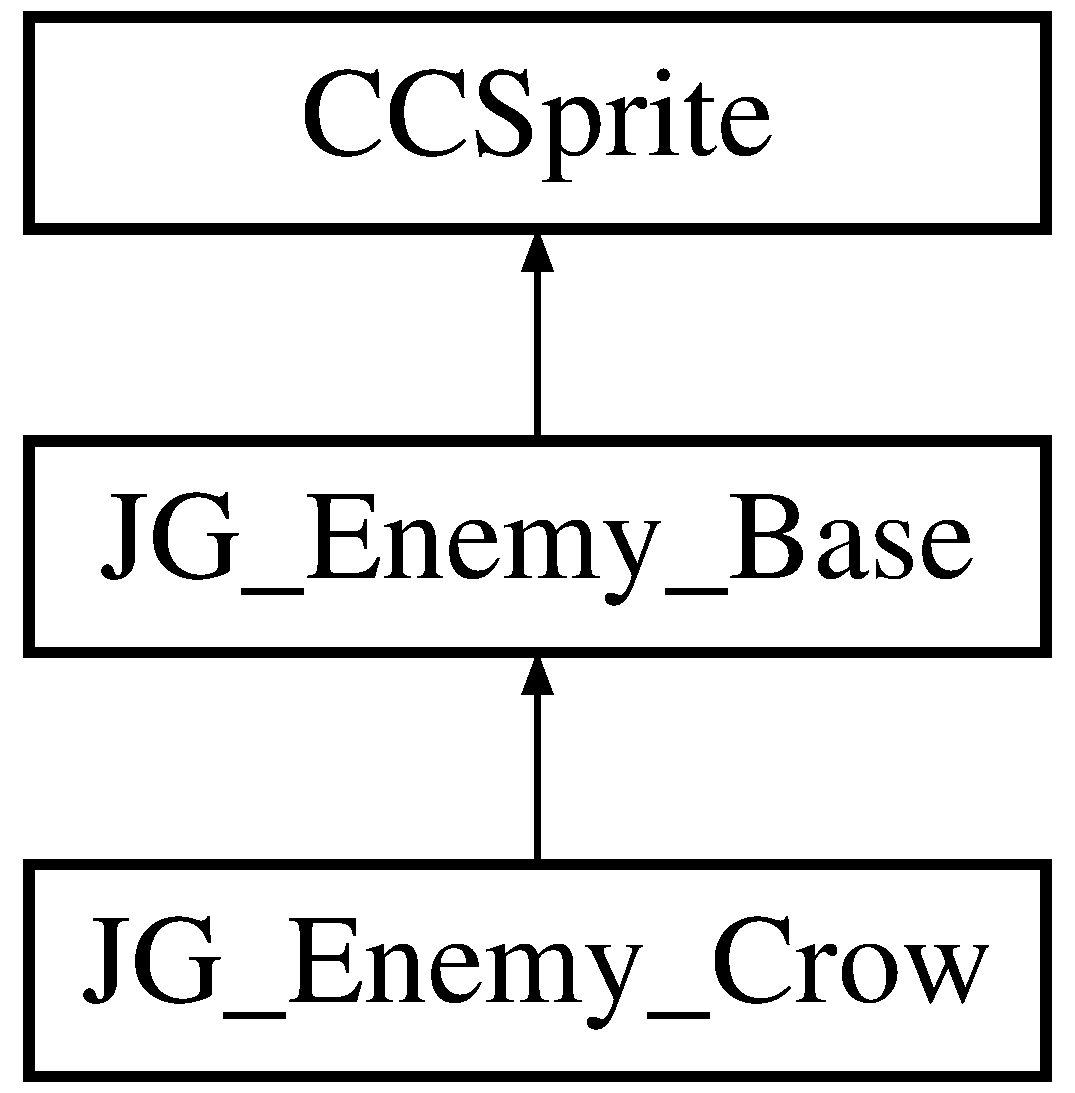
\includegraphics[height=3.000000cm]{class_j_g___enemy___crow}
\end{center}
\end{figure}
\subsection*{Additional Inherited Members}


The documentation for this class was generated from the following files\-:\begin{DoxyCompactItemize}
\item 
J\-G\-\_\-\-Enemy\-\_\-\-Crow.\-h\item 
J\-G\-\_\-\-Enemy\-\_\-\-Crow.\-cpp\end{DoxyCompactItemize}

\hypertarget{class_j_g___enemy___quick_attakc}{\section{J\-G\-\_\-\-Enemy\-\_\-\-Quick\-Attakc Class Reference}
\label{class_j_g___enemy___quick_attakc}\index{J\-G\-\_\-\-Enemy\-\_\-\-Quick\-Attakc@{J\-G\-\_\-\-Enemy\-\_\-\-Quick\-Attakc}}
}
Inheritance diagram for J\-G\-\_\-\-Enemy\-\_\-\-Quick\-Attakc\-:\begin{figure}[H]
\begin{center}
\leavevmode
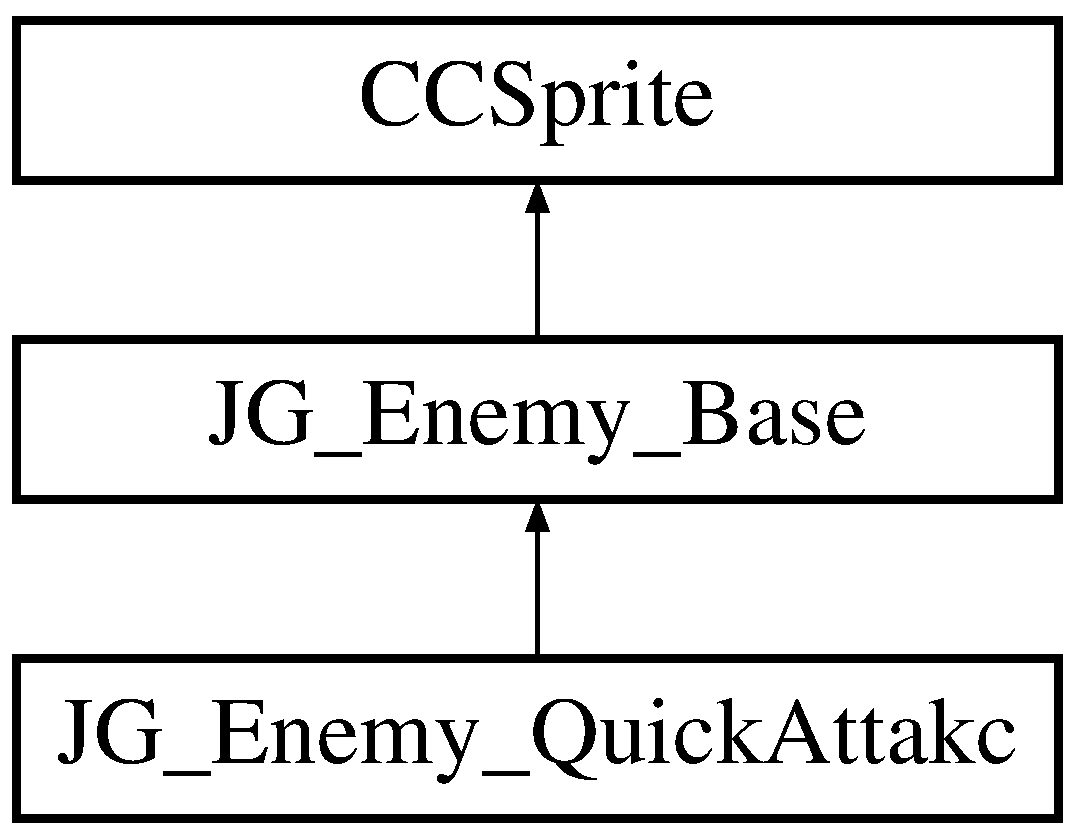
\includegraphics[height=3.000000cm]{class_j_g___enemy___quick_attakc}
\end{center}
\end{figure}
\subsection*{Additional Inherited Members}


The documentation for this class was generated from the following files\-:\begin{DoxyCompactItemize}
\item 
J\-G\-\_\-\-Enemy\-\_\-\-Quick\-Attakc.\-h\item 
J\-G\-\_\-\-Enemy\-\_\-\-Quick\-Attakc.\-cpp\end{DoxyCompactItemize}

\hypertarget{class_j_g___factory___attack_wave}{\section{J\-G\-\_\-\-Factory\-\_\-\-Attack\-Wave$<$ T $>$ Class Template Reference}
\label{class_j_g___factory___attack_wave}\index{J\-G\-\_\-\-Factory\-\_\-\-Attack\-Wave$<$ T $>$@{J\-G\-\_\-\-Factory\-\_\-\-Attack\-Wave$<$ T $>$}}
}
Inheritance diagram for J\-G\-\_\-\-Factory\-\_\-\-Attack\-Wave$<$ T $>$\-:\begin{figure}[H]
\begin{center}
\leavevmode
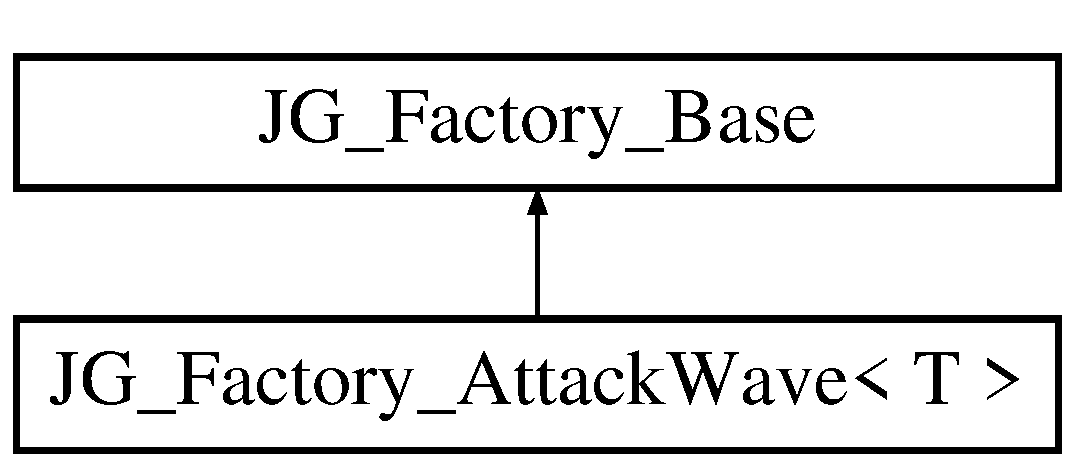
\includegraphics[height=2.000000cm]{class_j_g___factory___attack_wave}
\end{center}
\end{figure}
\subsection*{Public Member Functions}
\begin{DoxyCompactItemize}
\item 
\hypertarget{class_j_g___factory___attack_wave_a5d2f15ad078b1965dc98942fb601b895}{C\-C\-Node $\ast$ {\bfseries Create} ()}\label{class_j_g___factory___attack_wave_a5d2f15ad078b1965dc98942fb601b895}

\end{DoxyCompactItemize}


The documentation for this class was generated from the following file\-:\begin{DoxyCompactItemize}
\item 
J\-G\-\_\-\-Factory\-\_\-\-Attack\-Wave.\-h\end{DoxyCompactItemize}

\hypertarget{class_j_g___factory___base}{\section{J\-G\-\_\-\-Factory\-\_\-\-Base Class Reference}
\label{class_j_g___factory___base}\index{J\-G\-\_\-\-Factory\-\_\-\-Base@{J\-G\-\_\-\-Factory\-\_\-\-Base}}
}
Inheritance diagram for J\-G\-\_\-\-Factory\-\_\-\-Base\-:\begin{figure}[H]
\begin{center}
\leavevmode
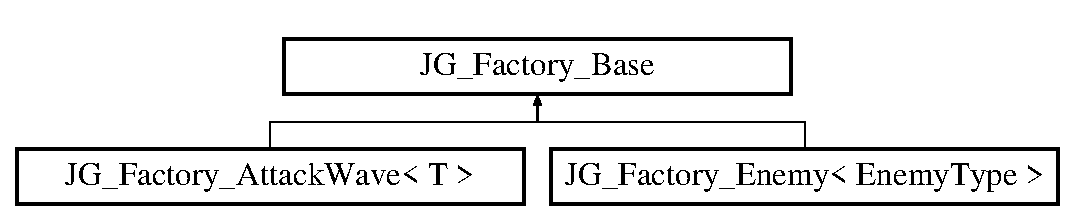
\includegraphics[height=2.000000cm]{class_j_g___factory___base}
\end{center}
\end{figure}
\subsection*{Public Member Functions}
\begin{DoxyCompactItemize}
\item 
\hypertarget{class_j_g___factory___base_af79850ce71f6e13af6d634fae32e862b}{virtual C\-C\-Node $\ast$ {\bfseries Create} ()=0}\label{class_j_g___factory___base_af79850ce71f6e13af6d634fae32e862b}

\end{DoxyCompactItemize}


The documentation for this class was generated from the following files\-:\begin{DoxyCompactItemize}
\item 
J\-G\-\_\-\-Factory\-\_\-\-Base.\-h\item 
J\-G\-\_\-\-Factory\-\_\-\-Base.\-cpp\end{DoxyCompactItemize}

\hypertarget{class_j_g___factory___enemy}{\section{J\-G\-\_\-\-Factory\-\_\-\-Enemy$<$ Enemy\-Type $>$ Class Template Reference}
\label{class_j_g___factory___enemy}\index{J\-G\-\_\-\-Factory\-\_\-\-Enemy$<$ Enemy\-Type $>$@{J\-G\-\_\-\-Factory\-\_\-\-Enemy$<$ Enemy\-Type $>$}}
}
Inheritance diagram for J\-G\-\_\-\-Factory\-\_\-\-Enemy$<$ Enemy\-Type $>$\-:\begin{figure}[H]
\begin{center}
\leavevmode
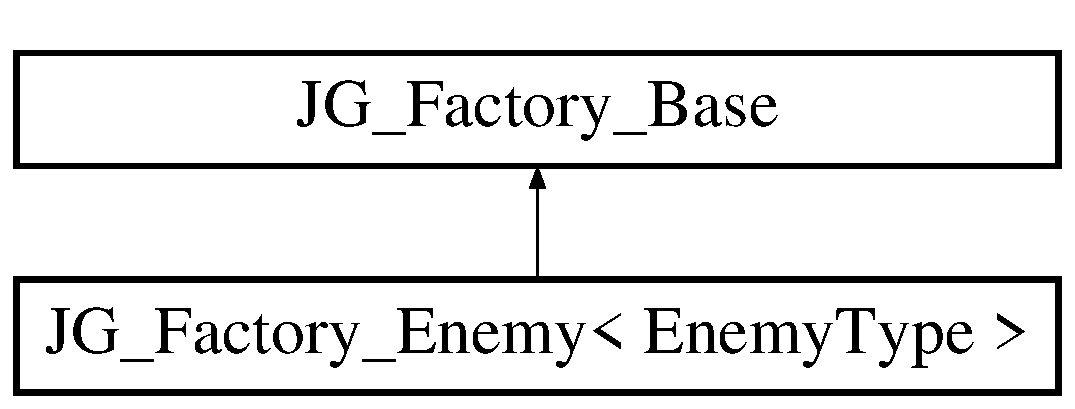
\includegraphics[height=2.000000cm]{class_j_g___factory___enemy}
\end{center}
\end{figure}
\subsection*{Public Member Functions}
\begin{DoxyCompactItemize}
\item 
\hypertarget{class_j_g___factory___enemy_afb37f360b552170832d8c55d42017c41}{C\-C\-Node $\ast$ {\bfseries Create} ()}\label{class_j_g___factory___enemy_afb37f360b552170832d8c55d42017c41}

\end{DoxyCompactItemize}


The documentation for this class was generated from the following file\-:\begin{DoxyCompactItemize}
\item 
J\-G\-\_\-\-Factory\-\_\-\-Enemy.\-h\end{DoxyCompactItemize}

\hypertarget{class_j_g___fruit}{\section{J\-G\-\_\-\-Fruit Class Reference}
\label{class_j_g___fruit}\index{J\-G\-\_\-\-Fruit@{J\-G\-\_\-\-Fruit}}
}
Inheritance diagram for J\-G\-\_\-\-Fruit\-:\begin{figure}[H]
\begin{center}
\leavevmode
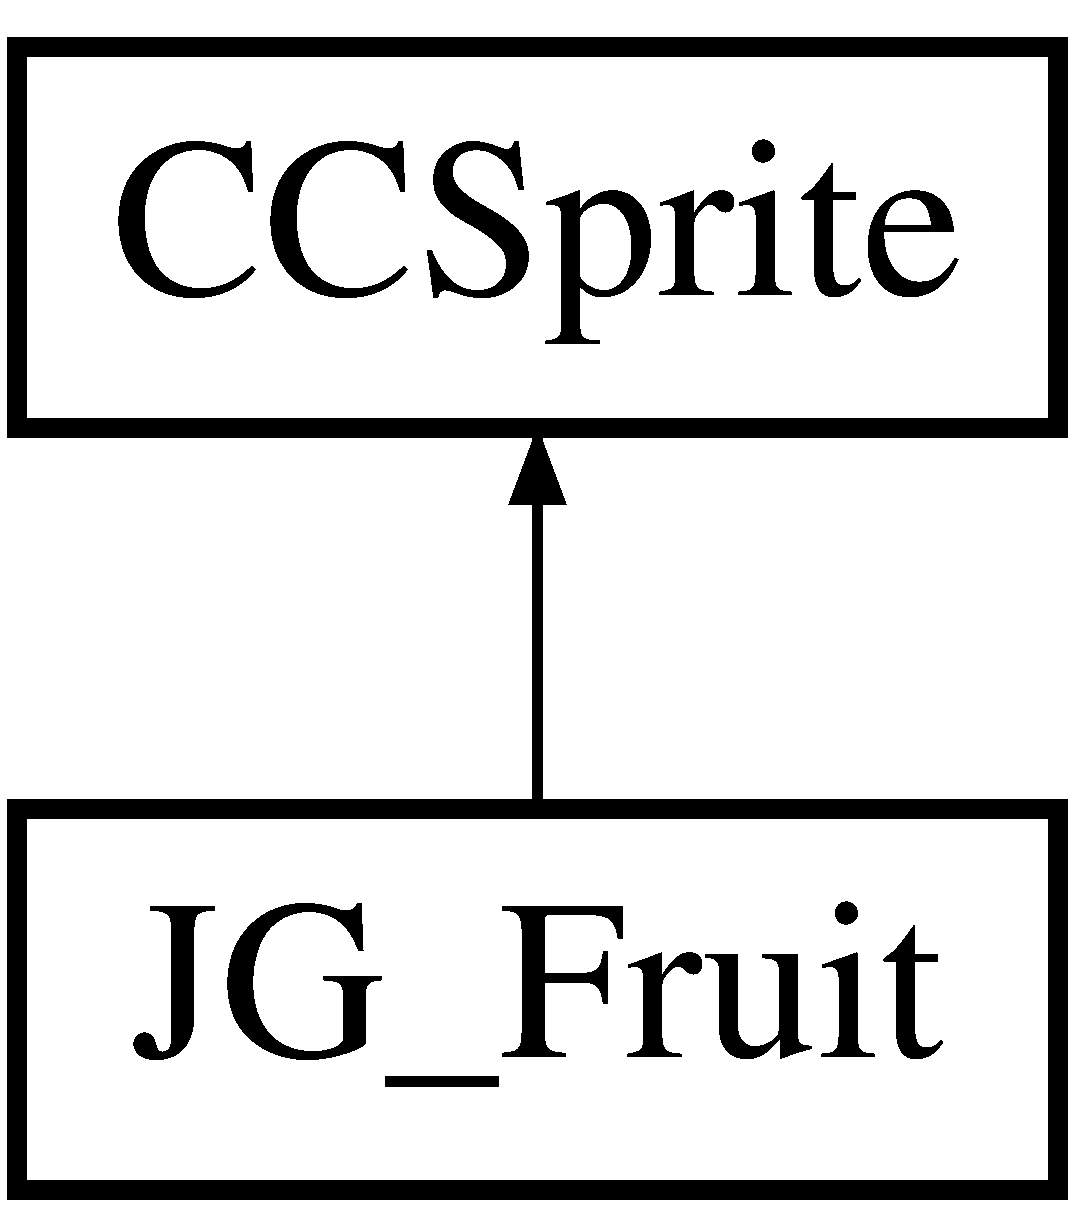
\includegraphics[height=2.000000cm]{class_j_g___fruit}
\end{center}
\end{figure}
\subsection*{Public Member Functions}
\begin{DoxyCompactItemize}
\item 
\hypertarget{class_j_g___fruit_a11c190fb214a37d7edc9b91a6ace714a}{void {\bfseries update} (float dt)}\label{class_j_g___fruit_a11c190fb214a37d7edc9b91a6ace714a}

\item 
\hypertarget{class_j_g___fruit_a5a9bac4669813237ffd8dd6445341371}{void {\bfseries Check\-Collision\-With\-Ball} ()}\label{class_j_g___fruit_a5a9bac4669813237ffd8dd6445341371}

\item 
\hypertarget{class_j_g___fruit_a98194a10c3f8001c3c57a05cd6a7665e}{void {\bfseries Process\-Move} (float dt)}\label{class_j_g___fruit_a98194a10c3f8001c3c57a05cd6a7665e}

\item 
\hypertarget{class_j_g___fruit_a222fabb403c98ddd762bbe8097271d61}{void {\bfseries Check\-Out\-Of\-Screen} ()}\label{class_j_g___fruit_a222fabb403c98ddd762bbe8097271d61}

\item 
\hypertarget{class_j_g___fruit_a373e8466f4394e7291082cc7ef064a8f}{float {\bfseries Get\-Score} ()}\label{class_j_g___fruit_a373e8466f4394e7291082cc7ef064a8f}

\end{DoxyCompactItemize}
\subsection*{Static Public Member Functions}
\begin{DoxyCompactItemize}
\item 
\hypertarget{class_j_g___fruit_a2fb42d26765781c6608a6f30cdc1f19b}{static \hyperlink{class_j_g___fruit}{J\-G\-\_\-\-Fruit} $\ast$ {\bfseries Create\-Fruit} (\hyperlink{class_j_g___game___main}{J\-G\-\_\-\-Game\-\_\-\-Main} $\ast$game, C\-C\-Point initial\-Position, float initial\-Speed)}\label{class_j_g___fruit_a2fb42d26765781c6608a6f30cdc1f19b}

\end{DoxyCompactItemize}


The documentation for this class was generated from the following files\-:\begin{DoxyCompactItemize}
\item 
J\-G\-\_\-\-Fruit.\-h\item 
J\-G\-\_\-\-Fruit.\-cpp\end{DoxyCompactItemize}

\hypertarget{class_j_g___game___g_u_i}{\section{J\-G\-\_\-\-Game\-\_\-\-G\-U\-I Class Reference}
\label{class_j_g___game___g_u_i}\index{J\-G\-\_\-\-Game\-\_\-\-G\-U\-I@{J\-G\-\_\-\-Game\-\_\-\-G\-U\-I}}
}
Inheritance diagram for J\-G\-\_\-\-Game\-\_\-\-G\-U\-I\-:\begin{figure}[H]
\begin{center}
\leavevmode
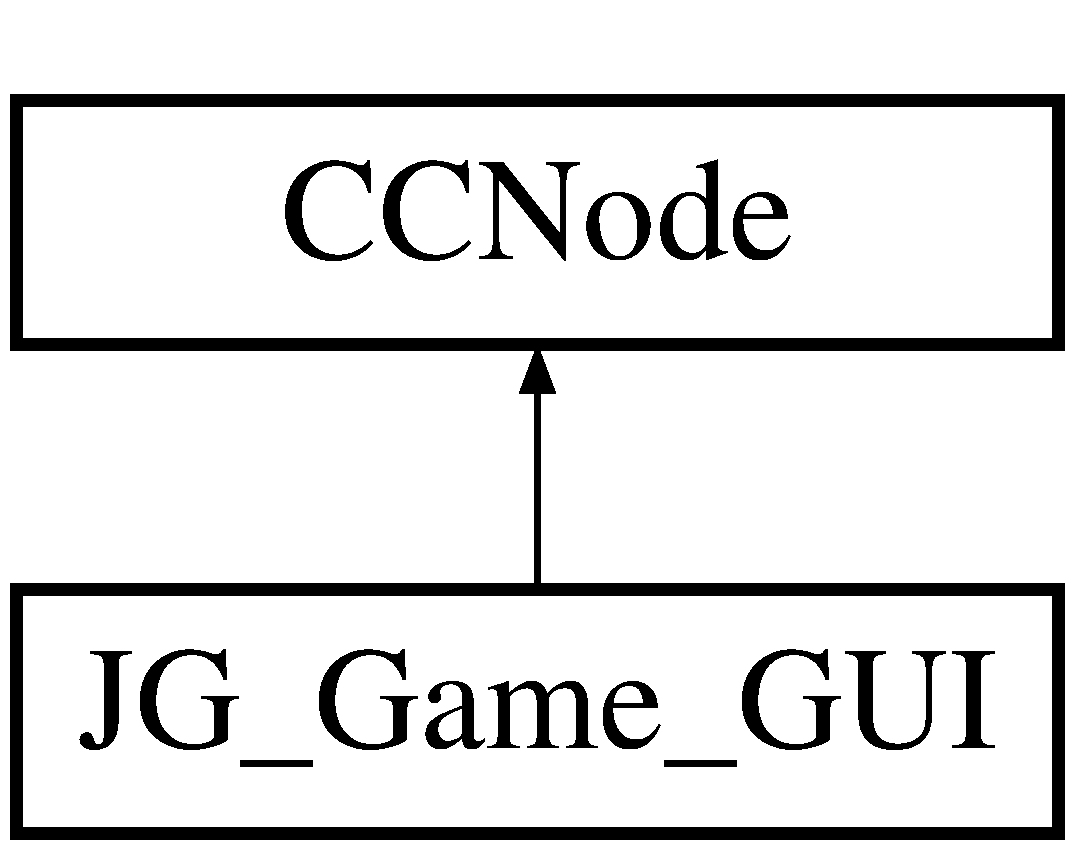
\includegraphics[height=2.000000cm]{class_j_g___game___g_u_i}
\end{center}
\end{figure}
\subsection*{Public Member Functions}
\begin{DoxyCompactItemize}
\item 
\hypertarget{class_j_g___game___g_u_i_ab796ce7767e6ab638449f6c5bd7ec905}{bool {\bfseries init} (\hyperlink{class_j_g___game___main}{J\-G\-\_\-\-Game\-\_\-\-Main} $\ast$game)}\label{class_j_g___game___g_u_i_ab796ce7767e6ab638449f6c5bd7ec905}

\item 
\hypertarget{class_j_g___game___g_u_i_a66308f118acf73c0bec5fa362e64a241}{void {\bfseries Init\-H\-U\-D\-Items} ()}\label{class_j_g___game___g_u_i_a66308f118acf73c0bec5fa362e64a241}

\item 
\hypertarget{class_j_g___game___g_u_i_a37b354adcbf5ac6cf3076b3c0f6d188d}{void {\bfseries Init\-Pause\-Menu\-Items} ()}\label{class_j_g___game___g_u_i_a37b354adcbf5ac6cf3076b3c0f6d188d}

\item 
\hypertarget{class_j_g___game___g_u_i_af4abc70383f754ee38e1e4c9d0e74de4}{void {\bfseries Init\-End\-Round\-Menu\-Items} ()}\label{class_j_g___game___g_u_i_af4abc70383f754ee38e1e4c9d0e74de4}

\item 
\hypertarget{class_j_g___game___g_u_i_a9d60bb38da03ace5804313a274d4ccb7}{void {\bfseries Init\-High\-Score\-Menu\-Items} ()}\label{class_j_g___game___g_u_i_a9d60bb38da03ace5804313a274d4ccb7}

\item 
\hypertarget{class_j_g___game___g_u_i_ac22f4e7566364d26fb4291dee43febb5}{void {\bfseries Set\-Pause\-Screen\-Visibility} (bool b\-Visible)}\label{class_j_g___game___g_u_i_ac22f4e7566364d26fb4291dee43febb5}

\item 
\hypertarget{class_j_g___game___g_u_i_ae0827ac4c62da200bd4dbef8cc84746d}{void {\bfseries Set\-High\-Score\-Screen\-Visibility} (bool b\-Visible)}\label{class_j_g___game___g_u_i_ae0827ac4c62da200bd4dbef8cc84746d}

\item 
\hypertarget{class_j_g___game___g_u_i_ad89a4556220ea6d5f6b974968efe21e2}{void {\bfseries Set\-End\-Round\-Screen\-Visibility} (bool b\-Visible)}\label{class_j_g___game___g_u_i_ad89a4556220ea6d5f6b974968efe21e2}

\item 
\hypertarget{class_j_g___game___g_u_i_aa1d4ffd2fb4eb61d3c5dd7e5e5e2b490}{void {\bfseries Set\-H\-U\-D\-Visibility} (bool b\-Visible)}\label{class_j_g___game___g_u_i_aa1d4ffd2fb4eb61d3c5dd7e5e5e2b490}

\item 
\hypertarget{class_j_g___game___g_u_i_a4c956efe3ed15d8e32d65affc2aa7a65}{void {\bfseries Hide\-G\-U\-I\-Screens} ()}\label{class_j_g___game___g_u_i_a4c956efe3ed15d8e32d65affc2aa7a65}

\item 
\hypertarget{class_j_g___game___g_u_i_a78d63ae05002fd82e1bcabf971f7a059}{void {\bfseries Set\-Debug\-Label\-Info} (std\-::string debug)}\label{class_j_g___game___g_u_i_a78d63ae05002fd82e1bcabf971f7a059}

\item 
\hypertarget{class_j_g___game___g_u_i_a57f38d08b8da17927d79eb50fa96695c}{void {\bfseries Reset\-Infos} ()}\label{class_j_g___game___g_u_i_a57f38d08b8da17927d79eb50fa96695c}

\item 
\hypertarget{class_j_g___game___g_u_i_aa1a358ee7434aa1c46e7b85a53e97f3f}{void {\bfseries draw} ()}\label{class_j_g___game___g_u_i_aa1a358ee7434aa1c46e7b85a53e97f3f}

\item 
\hypertarget{class_j_g___game___g_u_i_a250a8f4b46b5e20881564d87eebc87c4}{void {\bfseries Set\-End\-Round\-Screen\-Infos} (int \-\_\-player\-Score, int \-\_\-highest\-Score, C\-C\-String \-\_\-highest\-Score\-Player\-Name)}\label{class_j_g___game___g_u_i_a250a8f4b46b5e20881564d87eebc87c4}

\item 
\hypertarget{class_j_g___game___g_u_i_a6aeaa8103fe5e020189fccb30d29eddc}{void {\bfseries Set\-High\-Score\-Screen\-Infos} (int \-\_\-player\-Rank)}\label{class_j_g___game___g_u_i_a6aeaa8103fe5e020189fccb30d29eddc}

\item 
\hypertarget{class_j_g___game___g_u_i_afb682cc9a07f6d7feb9152b5cc5f14b6}{void {\bfseries Set\-Player\-Score} (int score)}\label{class_j_g___game___g_u_i_afb682cc9a07f6d7feb9152b5cc5f14b6}

\item 
\hypertarget{class_j_g___game___g_u_i_a59d66034539b81282ac21eeb05da2e4d}{void {\bfseries Set\-Player\-Reserved\-Ball} (int ball\-Count)}\label{class_j_g___game___g_u_i_a59d66034539b81282ac21eeb05da2e4d}

\item 
\hypertarget{class_j_g___game___g_u_i_a1ee44f474beb686224a7177789b41de0}{bool {\bfseries Is\-Player\-Name\-Text\-Box\-Visible} ()}\label{class_j_g___game___g_u_i_a1ee44f474beb686224a7177789b41de0}

\item 
\hypertarget{class_j_g___game___g_u_i_a1f02689e1fcf0219b4bbbd214d7d54a5}{void {\bfseries Check\-Player\-Name\-Text\-Box\-Touched} (C\-C\-Touch $\ast$touch)}\label{class_j_g___game___g_u_i_a1f02689e1fcf0219b4bbbd214d7d54a5}

\item 
\hypertarget{class_j_g___game___g_u_i_a2d092bd4b0e0aa3c2bd6da0e5e603d15}{std\-::string {\bfseries Get\-Player\-Name} ()}\label{class_j_g___game___g_u_i_a2d092bd4b0e0aa3c2bd6da0e5e603d15}

\end{DoxyCompactItemize}
\subsection*{Static Public Member Functions}
\begin{DoxyCompactItemize}
\item 
\hypertarget{class_j_g___game___g_u_i_a6559bb4b5a6c66faea5ac4c1e6ccc13b}{static \hyperlink{class_j_g___game___g_u_i}{J\-G\-\_\-\-Game\-\_\-\-G\-U\-I} $\ast$ {\bfseries create} (\hyperlink{class_j_g___game___main}{J\-G\-\_\-\-Game\-\_\-\-Main} $\ast$game)}\label{class_j_g___game___g_u_i_a6559bb4b5a6c66faea5ac4c1e6ccc13b}

\end{DoxyCompactItemize}
\subsection*{Public Attributes}
\begin{DoxyCompactItemize}
\item 
\hypertarget{class_j_g___game___g_u_i_aee99def04073afd98b756ac85a858f76}{C\-C\-Menu\-Item\-Sprite $\ast$ {\bfseries pause\-Button}}\label{class_j_g___game___g_u_i_aee99def04073afd98b756ac85a858f76}

\item 
\hypertarget{class_j_g___game___g_u_i_a548c9060d30306a25a3656f11f653dfb}{C\-C\-Menu\-Item\-Sprite $\ast$ {\bfseries reset\-Button}}\label{class_j_g___game___g_u_i_a548c9060d30306a25a3656f11f653dfb}

\item 
\hypertarget{class_j_g___game___g_u_i_a3397236c35ec22aa7d8e3fcfa8d894a1}{C\-C\-Menu\-Item\-Sprite $\ast$ {\bfseries resume\-Button}}\label{class_j_g___game___g_u_i_a3397236c35ec22aa7d8e3fcfa8d894a1}

\item 
\hypertarget{class_j_g___game___g_u_i_a566545f07da25832efb00d458fc832e7}{C\-C\-Menu\-Item\-Sprite $\ast$ {\bfseries exit\-Game\-Button}}\label{class_j_g___game___g_u_i_a566545f07da25832efb00d458fc832e7}

\item 
\hypertarget{class_j_g___game___g_u_i_abebe14e53b373f190631d734fcda5813}{C\-C\-Menu\-Item\-Sprite $\ast$ {\bfseries exit\-To\-Main\-Menu\-Button}}\label{class_j_g___game___g_u_i_abebe14e53b373f190631d734fcda5813}

\item 
\hypertarget{class_j_g___game___g_u_i_a333b3b0725e8ffeb8ac1583577871712}{C\-C\-Menu\-Item\-Sprite $\ast$ {\bfseries ball\-Add\-Button}}\label{class_j_g___game___g_u_i_a333b3b0725e8ffeb8ac1583577871712}

\item 
\hypertarget{class_j_g___game___g_u_i_a14906deb34d982fac0518919b2020c6c}{C\-C\-Menu\-Item\-Sprite $\ast$ {\bfseries end\-Round\-\_\-\-Retry\-Button}}\label{class_j_g___game___g_u_i_a14906deb34d982fac0518919b2020c6c}

\item 
\hypertarget{class_j_g___game___g_u_i_a46599fe066ad468c56b0fac58fdccd1c}{C\-C\-Menu\-Item\-Sprite $\ast$ {\bfseries end\-Round\-\_\-\-Exit\-To\-Menu\-Button}}\label{class_j_g___game___g_u_i_a46599fe066ad468c56b0fac58fdccd1c}

\item 
\hypertarget{class_j_g___game___g_u_i_a53e3b8174b2ebd433cb9ed753d5e5c2c}{C\-C\-Label\-B\-M\-Font $\ast$ {\bfseries score\-Label}}\label{class_j_g___game___g_u_i_a53e3b8174b2ebd433cb9ed753d5e5c2c}

\item 
\hypertarget{class_j_g___game___g_u_i_ae88bbd163193cef29f94673d4845eb6e}{C\-C\-Label\-B\-M\-Font $\ast$ {\bfseries reserved\-Ball\-Label}}\label{class_j_g___game___g_u_i_ae88bbd163193cef29f94673d4845eb6e}

\item 
\hypertarget{class_j_g___game___g_u_i_af9213ca3a5f5c427971e54ab32c5cf43}{C\-C\-Label\-B\-M\-Font $\ast$ {\bfseries highest\-Score\-Label}}\label{class_j_g___game___g_u_i_af9213ca3a5f5c427971e54ab32c5cf43}

\item 
\hypertarget{class_j_g___game___g_u_i_a86b1a5c05686a9173208d9a609339ebd}{C\-C\-Label\-B\-M\-Font $\ast$ {\bfseries player\-Final\-Score\-Label}}\label{class_j_g___game___g_u_i_a86b1a5c05686a9173208d9a609339ebd}

\item 
\hypertarget{class_j_g___game___g_u_i_a033275d4174f6f61d5dcbf17920e875f}{C\-C\-Label\-B\-M\-Font $\ast$ {\bfseries player\-Rank\-Label}}\label{class_j_g___game___g_u_i_a033275d4174f6f61d5dcbf17920e875f}

\item 
\hypertarget{class_j_g___game___g_u_i_ac88e0f0c5ab46ab45f28a2562ed06722}{C\-C\-Text\-Field\-T\-T\-F $\ast$ {\bfseries player\-Name\-Text\-Box}}\label{class_j_g___game___g_u_i_ac88e0f0c5ab46ab45f28a2562ed06722}

\item 
\hypertarget{class_j_g___game___g_u_i_a5fc5adc75e567a55869c196844cf073b}{C\-C\-Label\-B\-M\-Font $\ast$ {\bfseries debug\-Label}}\label{class_j_g___game___g_u_i_a5fc5adc75e567a55869c196844cf073b}

\item 
\hypertarget{class_j_g___game___g_u_i_a886cd9bd4a12da25e1f05ca9e1a501ce}{C\-C\-Point {\bfseries life\-Draw\-Position}}\label{class_j_g___game___g_u_i_a886cd9bd4a12da25e1f05ca9e1a501ce}

\item 
\hypertarget{class_j_g___game___g_u_i_a69435a812e22fa55dce2f24f2312ee2c}{int {\bfseries life\-Draw\-Pacing}}\label{class_j_g___game___g_u_i_a69435a812e22fa55dce2f24f2312ee2c}

\item 
\hypertarget{class_j_g___game___g_u_i_a77dac1b5580d1d1476a73a2ae954e1ec}{C\-C\-Texture2\-D $\ast$ {\bfseries life\-Texture\-\_\-\-Active}}\label{class_j_g___game___g_u_i_a77dac1b5580d1d1476a73a2ae954e1ec}

\item 
\hypertarget{class_j_g___game___g_u_i_a9d5b10e0006ec907f28bf56b24445108}{C\-C\-Texture2\-D $\ast$ {\bfseries life\-Texture\-\_\-\-Diactive}}\label{class_j_g___game___g_u_i_a9d5b10e0006ec907f28bf56b24445108}

\item 
\hypertarget{class_j_g___game___g_u_i_afea3a0ffb12113d009ed39c1bedd2727}{C\-C\-Finite\-Time\-Action $\ast$ {\bfseries Score\-Gain\-Animation}}\label{class_j_g___game___g_u_i_afea3a0ffb12113d009ed39c1bedd2727}

\end{DoxyCompactItemize}


The documentation for this class was generated from the following files\-:\begin{DoxyCompactItemize}
\item 
J\-G\-\_\-\-Game\-\_\-\-G\-U\-I.\-h\item 
J\-G\-\_\-\-Game\-\_\-\-G\-U\-I.\-cpp\end{DoxyCompactItemize}

\hypertarget{class_j_g___game___main}{\section{J\-G\-\_\-\-Game\-\_\-\-Main Class Reference}
\label{class_j_g___game___main}\index{J\-G\-\_\-\-Game\-\_\-\-Main@{J\-G\-\_\-\-Game\-\_\-\-Main}}
}


{\ttfamily \#include $<$J\-G\-\_\-\-Game\-\_\-\-Main.\-h$>$}

Inheritance diagram for J\-G\-\_\-\-Game\-\_\-\-Main\-:\begin{figure}[H]
\begin{center}
\leavevmode
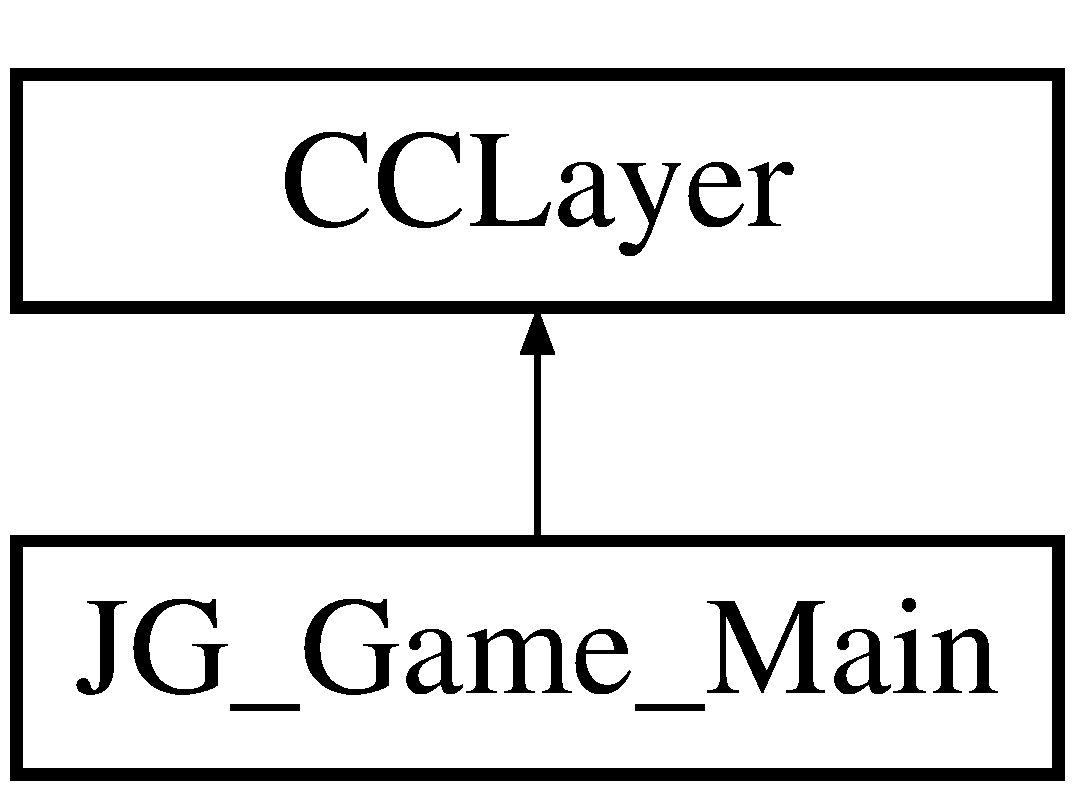
\includegraphics[height=2.000000cm]{class_j_g___game___main}
\end{center}
\end{figure}
\subsection*{Public Member Functions}
\begin{DoxyCompactItemize}
\item 
void \hyperlink{class_j_g___game___main_a36ec5b32f8d745363bafa97dbcfc63fd}{Ball\-Lost} (\hyperlink{class_j_g___ball}{J\-G\-\_\-\-Ball} $\ast$lost\-Ball)
\item 
int \hyperlink{class_j_g___game___main_afa38293cf043c824ccfa4aebe1e1545f}{Get\-Score} ()
\item 
void \hyperlink{class_j_g___game___main_a565135339ab0e993ace77fbfc8b39ab2}{Set\-Score} (int new\-Score)
\item 
void \hyperlink{class_j_g___game___main_af1018c29931a8569a468b0b7495ca5cc}{Add\-Score} (int amount)
\item 
void \hyperlink{class_j_g___game___main_a30a9fb93f7a2a61ce90ab1a77525c006}{Reduce\-Score} (int amount)
\item 
int \hyperlink{class_j_g___game___main_a666b141713d126df7e171fc68dd257a2}{Get\-Life\-Count} ()
\item 
void \hyperlink{class_j_g___game___main_a80e74d397b65b98182fb5c2054632899}{Set\-Life\-Count} (int new\-Life\-Count)
\item 
void \hyperlink{class_j_g___game___main_abffce98f5d7c28791aa13e4d081da6ec}{Decrement\-Life\-Count} ()
\item 
void \hyperlink{class_j_g___game___main_a529a8f577bb296cbbe9143f99ae26f1b}{Increment\-Life\-Count} ()
\item 
\hypertarget{class_j_g___game___main_a4d1e63d731fabbe9e57383254a4b21bf}{virtual bool {\bfseries init} ()}\label{class_j_g___game___main_a4d1e63d731fabbe9e57383254a4b21bf}

\item 
void \hyperlink{class_j_g___game___main_ab7f59e22bd1ddc6f849ceb4731e6f123}{Init\-Game} ()
\item 
virtual void \hyperlink{class_j_g___game___main_a9c8aac91fd97b7a88da7819b8ead4206}{cc\-Touches\-Began} (C\-C\-Set $\ast$p\-Touches, C\-C\-Event $\ast$event)
\item 
virtual void \hyperlink{class_j_g___game___main_ad3ecad4bd190ff37f5b6ba1da9fbe16c}{cc\-Touches\-Moved} (C\-C\-Set $\ast$p\-Touches, C\-C\-Event $\ast$event)
\item 
virtual void \hyperlink{class_j_g___game___main_a0bc1f108b8a56226cfe84ce9d28d56b4}{cc\-Touches\-Ended} (C\-C\-Set $\ast$p\-Touches, C\-C\-Event $\ast$event)
\item 
void \hyperlink{class_j_g___game___main_afe6f0284267c514ca1c81673d015ad91}{Ball\-Touch\-Handler\-\_\-\-Init} (C\-C\-Touch $\ast$touch)
\item 
void \hyperlink{class_j_g___game___main_aa0d9b99e2acd78c8763557d1c0e8a244}{Ball\-Touch\-Handler\-\_\-\-Check\-Direction} (unsigned int index)
\item 
void \hyperlink{class_j_g___game___main_af02d329a7f3a6ac86d8b233dd9ff0741}{Ball\-Touch\-Handler\-\_\-\-End} (unsigned int index)
\item 
void \hyperlink{class_j_g___game___main_a4accf9781acdb8a94450eca925574902}{Ball\-Touch\-Handler\-\_\-\-Check\-Time} (float dt)
\item 
float \hyperlink{class_j_g___game___main_a3b28b2a51aeaa909d6fb95471103bb72}{Calculate\-Throw\-Force} (unsigned int index)
\item 
void \hyperlink{class_j_g___game___main_aea78b9aef2cf228b6945fa88bf741c3a}{update} (float dt)
\item 
bool \hyperlink{class_j_g___game___main_a0b93b253ff5f67b688c12848c63c9e2c}{Are\-Points\-Colliding} (C\-C\-Point point1, C\-C\-Point point2, float radius)
\item 
void \hyperlink{class_j_g___game___main_abda6daf16a4bdfb1d197bcedce380f8e}{Set\-Touch\-Info} (C\-C\-Touch $\ast$touch, \hyperlink{class_j_g___hand}{J\-G\-\_\-\-Hand} $\ast$hand, \hyperlink{class_j_g___ball}{J\-G\-\_\-\-Ball} $\ast$ball)
\item 
void \hyperlink{class_j_g___game___main_a24a120d001b984dc67f211cdb79ce811}{Reset\-Touch\-Info} (int index)
\item 
void \hyperlink{class_j_g___game___main_a2f8dd795fb006e6b052dbe29aef917cf}{Reset\-Touch\-Info\-By\-Ball} (\hyperlink{class_j_g___ball}{J\-G\-\_\-\-Ball} $\ast$ball)
\item 
bool \hyperlink{class_j_g___game___main_a0fab6585f29f1324aea00bdade4e01f4}{Set\-Touch\-Direction\-For\-Ball} (int index)
\item 
\hypertarget{class_j_g___game___main_a42558255c3477748cfadf9d501a02b56}{void {\bfseries menu\-Close\-Callback} (C\-C\-Object $\ast$p\-Sender)}\label{class_j_g___game___main_a42558255c3477748cfadf9d501a02b56}

\item 
\hypertarget{class_j_g___game___main_a2e2740b51a8e5ac7b981078dbd7bbd70}{void {\bfseries menu\-Pause\-Call\-Back} (C\-C\-Object $\ast$p\-Sender)}\label{class_j_g___game___main_a2e2740b51a8e5ac7b981078dbd7bbd70}

\item 
void \hyperlink{class_j_g___game___main_adc1658ea07b4deb55bfe22df04b61aa2}{Remove\-Ball\-From\-Screen} (\hyperlink{class_j_g___ball}{J\-G\-\_\-\-Ball} $\ast$ball)
\item 
void \hyperlink{class_j_g___game___main_a3b5871764fe94896c274e2a072c00dda}{Remove\-All\-Balls\-From\-Screen} ()
\item 
void \hyperlink{class_j_g___game___main_ae827327aa2c6e58cee824a6f5010f5fe}{Add\-Ball\-To\-Screen} ()
\item 
\hypertarget{class_j_g___game___main_aa386bd7cdada1f23b0b32526e67cc2b0}{float {\bfseries get\-Sign} (float num)}\label{class_j_g___game___main_aa386bd7cdada1f23b0b32526e67cc2b0}

\item 
\hypertarget{class_j_g___game___main_ad94a26b81515a717556314a3a8c65b31}{{\bfseries C\-R\-E\-A\-T\-E\-\_\-\-F\-U\-N\-C} (\hyperlink{class_j_g___game___main}{J\-G\-\_\-\-Game\-\_\-\-Main})}\label{class_j_g___game___main_ad94a26b81515a717556314a3a8c65b31}

\item 
void \hyperlink{class_j_g___game___main_ad4691efc615e12254ea347a7b21cd167}{Test\-Single\-Touch} ()
\item 
void \hyperlink{class_j_g___game___main_a5ad7dc858f795f34d33c13b712880b43}{Test\-Multi\-Touch} ()
\item 
void \hyperlink{class_j_g___game___main_a104c8ad94eb551ad2ba292aa46c0298c}{Test\-Multi\-Touch\-\_\-\-Initi\-Touch\-Gen} (float dt=0)
\item 
void \hyperlink{class_j_g___game___main_ae410c7d1cc74a9e7bf6bc51b525f889e}{Test\-Multi\-Touch\-\_\-\-Movement\-Touch\-Gen} (float dt=0)
\item 
void \hyperlink{class_j_g___game___main_ab2d7fb8240de8466d624a2f187d5eadf}{Test\-Multi\-Touch\-\_\-\-End\-Gen} (float dt=0)
\item 
void \hyperlink{class_j_g___game___main_a925a777f7a94c35b278434ff642b623b}{End\-Game} ()
\item 
void \hyperlink{class_j_g___game___main_a511aee5105b667f9d781030e1bdd7d16}{Pause\-Game} (C\-C\-Object $\ast$p\-Sender)
\item 
void \hyperlink{class_j_g___game___main_ad7a6bcb044fcd6f415bf005b8682de9b}{Exit\-Game} (C\-C\-Object $\ast$p\-Sender)
\item 
void \hyperlink{class_j_g___game___main_a0e1494d3e5c8c0a22f0d202716923839}{Resume\-Game} (C\-C\-Object $\ast$p\-Sender)
\item 
void \hyperlink{class_j_g___game___main_a186a53d9b5956462dd186a48adaf251c}{Reset\-Game} (C\-C\-Object $\ast$p\-Sender)
\item 
\hypertarget{class_j_g___game___main_abbbc10c904cdcba09260c925c36d0f22}{void {\bfseries Temp\-Add\-Ball} (float time)}\label{class_j_g___game___main_abbbc10c904cdcba09260c925c36d0f22}

\end{DoxyCompactItemize}
\subsection*{Static Public Member Functions}
\begin{DoxyCompactItemize}
\item 
\hypertarget{class_j_g___game___main_ad8df9f7dc524c5e4096ba72ca3d225a0}{static cocos2d\-::\-C\-C\-Scene $\ast$ {\bfseries scene} ()}\label{class_j_g___game___main_ad8df9f7dc524c5e4096ba72ca3d225a0}

\end{DoxyCompactItemize}
\subsection*{Public Attributes}
\begin{DoxyCompactItemize}
\item 
\hypertarget{class_j_g___game___main_a3312f494aeb62375e2ba54cfc2e7b4f9}{\hyperlink{class_j_g___game___h_u_d}{J\-G\-\_\-\-Game\-\_\-\-H\-U\-D} $\ast$ {\bfseries game\-H\-U\-D}}\label{class_j_g___game___main_a3312f494aeb62375e2ba54cfc2e7b4f9}

\item 
\hypertarget{class_j_g___game___main_a6946a041c2d1e0e1af8f668df4eaef1d}{int {\bfseries life\-Count}}\label{class_j_g___game___main_a6946a041c2d1e0e1af8f668df4eaef1d}

\item 
\hypertarget{class_j_g___game___main_a092aed9f82afd093223436207aaf95ee}{int {\bfseries score}}\label{class_j_g___game___main_a092aed9f82afd093223436207aaf95ee}

\item 
\hypertarget{class_j_g___game___main_a8974bfdd52077060e4561210cabd193f}{C\-C\-Size {\bfseries screen\-Size}}\label{class_j_g___game___main_a8974bfdd52077060e4561210cabd193f}

\item 
C\-C\-Set $\ast$ \hyperlink{class_j_g___game___main_abf4ca18c92688188dcf7bf60c73fa3ae}{Test\-Multi\-Touches\-Set}
\end{DoxyCompactItemize}


\subsection{Detailed Description}
The main class for controlling the game 

\subsection{Member Function Documentation}
\hypertarget{class_j_g___game___main_ae827327aa2c6e58cee824a6f5010f5fe}{\index{J\-G\-\_\-\-Game\-\_\-\-Main@{J\-G\-\_\-\-Game\-\_\-\-Main}!Add\-Ball\-To\-Screen@{Add\-Ball\-To\-Screen}}
\index{Add\-Ball\-To\-Screen@{Add\-Ball\-To\-Screen}!JG_Game_Main@{J\-G\-\_\-\-Game\-\_\-\-Main}}
\subsubsection[{Add\-Ball\-To\-Screen}]{\setlength{\rightskip}{0pt plus 5cm}void J\-G\-\_\-\-Game\-\_\-\-Main\-::\-Add\-Ball\-To\-Screen (
\begin{DoxyParamCaption}
{}
\end{DoxyParamCaption}
)}}\label{class_j_g___game___main_ae827327aa2c6e58cee824a6f5010f5fe}
Adding new ball to screen \hypertarget{class_j_g___game___main_af1018c29931a8569a468b0b7495ca5cc}{\index{J\-G\-\_\-\-Game\-\_\-\-Main@{J\-G\-\_\-\-Game\-\_\-\-Main}!Add\-Score@{Add\-Score}}
\index{Add\-Score@{Add\-Score}!JG_Game_Main@{J\-G\-\_\-\-Game\-\_\-\-Main}}
\subsubsection[{Add\-Score}]{\setlength{\rightskip}{0pt plus 5cm}void J\-G\-\_\-\-Game\-\_\-\-Main\-::\-Add\-Score (
\begin{DoxyParamCaption}
\item[{int}]{amount}
\end{DoxyParamCaption}
)}}\label{class_j_g___game___main_af1018c29931a8569a468b0b7495ca5cc}
Add a value to player score \hypertarget{class_j_g___game___main_a0b93b253ff5f67b688c12848c63c9e2c}{\index{J\-G\-\_\-\-Game\-\_\-\-Main@{J\-G\-\_\-\-Game\-\_\-\-Main}!Are\-Points\-Colliding@{Are\-Points\-Colliding}}
\index{Are\-Points\-Colliding@{Are\-Points\-Colliding}!JG_Game_Main@{J\-G\-\_\-\-Game\-\_\-\-Main}}
\subsubsection[{Are\-Points\-Colliding}]{\setlength{\rightskip}{0pt plus 5cm}bool J\-G\-\_\-\-Game\-\_\-\-Main\-::\-Are\-Points\-Colliding (
\begin{DoxyParamCaption}
\item[{C\-C\-Point}]{point1, }
\item[{C\-C\-Point}]{point2, }
\item[{float}]{radius}
\end{DoxyParamCaption}
)}}\label{class_j_g___game___main_a0b93b253ff5f67b688c12848c63c9e2c}
checks whether distance of the two point are lesser than radius or not \hypertarget{class_j_g___game___main_a36ec5b32f8d745363bafa97dbcfc63fd}{\index{J\-G\-\_\-\-Game\-\_\-\-Main@{J\-G\-\_\-\-Game\-\_\-\-Main}!Ball\-Lost@{Ball\-Lost}}
\index{Ball\-Lost@{Ball\-Lost}!JG_Game_Main@{J\-G\-\_\-\-Game\-\_\-\-Main}}
\subsubsection[{Ball\-Lost}]{\setlength{\rightskip}{0pt plus 5cm}void J\-G\-\_\-\-Game\-\_\-\-Main\-::\-Ball\-Lost (
\begin{DoxyParamCaption}
\item[{{\bf J\-G\-\_\-\-Ball} $\ast$}]{lost\-Ball}
\end{DoxyParamCaption}
)}}\label{class_j_g___game___main_a36ec5b32f8d745363bafa97dbcfc63fd}
this method is called when a ball is lost ( for now when it is out of screen ) \hypertarget{class_j_g___game___main_aa0d9b99e2acd78c8763557d1c0e8a244}{\index{J\-G\-\_\-\-Game\-\_\-\-Main@{J\-G\-\_\-\-Game\-\_\-\-Main}!Ball\-Touch\-Handler\-\_\-\-Check\-Direction@{Ball\-Touch\-Handler\-\_\-\-Check\-Direction}}
\index{Ball\-Touch\-Handler\-\_\-\-Check\-Direction@{Ball\-Touch\-Handler\-\_\-\-Check\-Direction}!JG_Game_Main@{J\-G\-\_\-\-Game\-\_\-\-Main}}
\subsubsection[{Ball\-Touch\-Handler\-\_\-\-Check\-Direction}]{\setlength{\rightskip}{0pt plus 5cm}void J\-G\-\_\-\-Game\-\_\-\-Main\-::\-Ball\-Touch\-Handler\-\_\-\-Check\-Direction (
\begin{DoxyParamCaption}
\item[{unsigned int}]{index}
\end{DoxyParamCaption}
)}}\label{class_j_g___game___main_aa0d9b99e2acd78c8763557d1c0e8a244}
check direction of the ball \hypertarget{class_j_g___game___main_a4accf9781acdb8a94450eca925574902}{\index{J\-G\-\_\-\-Game\-\_\-\-Main@{J\-G\-\_\-\-Game\-\_\-\-Main}!Ball\-Touch\-Handler\-\_\-\-Check\-Time@{Ball\-Touch\-Handler\-\_\-\-Check\-Time}}
\index{Ball\-Touch\-Handler\-\_\-\-Check\-Time@{Ball\-Touch\-Handler\-\_\-\-Check\-Time}!JG_Game_Main@{J\-G\-\_\-\-Game\-\_\-\-Main}}
\subsubsection[{Ball\-Touch\-Handler\-\_\-\-Check\-Time}]{\setlength{\rightskip}{0pt plus 5cm}void J\-G\-\_\-\-Game\-\_\-\-Main\-::\-Ball\-Touch\-Handler\-\_\-\-Check\-Time (
\begin{DoxyParamCaption}
\item[{float}]{dt}
\end{DoxyParamCaption}
)}}\label{class_j_g___game___main_a4accf9781acdb8a94450eca925574902}
it handle the time player hold his touch on the screen \hypertarget{class_j_g___game___main_af02d329a7f3a6ac86d8b233dd9ff0741}{\index{J\-G\-\_\-\-Game\-\_\-\-Main@{J\-G\-\_\-\-Game\-\_\-\-Main}!Ball\-Touch\-Handler\-\_\-\-End@{Ball\-Touch\-Handler\-\_\-\-End}}
\index{Ball\-Touch\-Handler\-\_\-\-End@{Ball\-Touch\-Handler\-\_\-\-End}!JG_Game_Main@{J\-G\-\_\-\-Game\-\_\-\-Main}}
\subsubsection[{Ball\-Touch\-Handler\-\_\-\-End}]{\setlength{\rightskip}{0pt plus 5cm}void J\-G\-\_\-\-Game\-\_\-\-Main\-::\-Ball\-Touch\-Handler\-\_\-\-End (
\begin{DoxyParamCaption}
\item[{unsigned int}]{index}
\end{DoxyParamCaption}
)}}\label{class_j_g___game___main_af02d329a7f3a6ac86d8b233dd9ff0741}
handling the throwing of the ball \hypertarget{class_j_g___game___main_afe6f0284267c514ca1c81673d015ad91}{\index{J\-G\-\_\-\-Game\-\_\-\-Main@{J\-G\-\_\-\-Game\-\_\-\-Main}!Ball\-Touch\-Handler\-\_\-\-Init@{Ball\-Touch\-Handler\-\_\-\-Init}}
\index{Ball\-Touch\-Handler\-\_\-\-Init@{Ball\-Touch\-Handler\-\_\-\-Init}!JG_Game_Main@{J\-G\-\_\-\-Game\-\_\-\-Main}}
\subsubsection[{Ball\-Touch\-Handler\-\_\-\-Init}]{\setlength{\rightskip}{0pt plus 5cm}void J\-G\-\_\-\-Game\-\_\-\-Main\-::\-Ball\-Touch\-Handler\-\_\-\-Init (
\begin{DoxyParamCaption}
\item[{C\-C\-Touch $\ast$}]{touch}
\end{DoxyParamCaption}
)}}\label{class_j_g___game___main_afe6f0284267c514ca1c81673d015ad91}
defined to handle initiation of touch \hypertarget{class_j_g___game___main_a3b28b2a51aeaa909d6fb95471103bb72}{\index{J\-G\-\_\-\-Game\-\_\-\-Main@{J\-G\-\_\-\-Game\-\_\-\-Main}!Calculate\-Throw\-Force@{Calculate\-Throw\-Force}}
\index{Calculate\-Throw\-Force@{Calculate\-Throw\-Force}!JG_Game_Main@{J\-G\-\_\-\-Game\-\_\-\-Main}}
\subsubsection[{Calculate\-Throw\-Force}]{\setlength{\rightskip}{0pt plus 5cm}float J\-G\-\_\-\-Game\-\_\-\-Main\-::\-Calculate\-Throw\-Force (
\begin{DoxyParamCaption}
\item[{unsigned int}]{index}
\end{DoxyParamCaption}
)}}\label{class_j_g___game___main_a3b28b2a51aeaa909d6fb95471103bb72}
to calculate the force of the touch \hypertarget{class_j_g___game___main_a9c8aac91fd97b7a88da7819b8ead4206}{\index{J\-G\-\_\-\-Game\-\_\-\-Main@{J\-G\-\_\-\-Game\-\_\-\-Main}!cc\-Touches\-Began@{cc\-Touches\-Began}}
\index{cc\-Touches\-Began@{cc\-Touches\-Began}!JG_Game_Main@{J\-G\-\_\-\-Game\-\_\-\-Main}}
\subsubsection[{cc\-Touches\-Began}]{\setlength{\rightskip}{0pt plus 5cm}void J\-G\-\_\-\-Game\-\_\-\-Main\-::cc\-Touches\-Began (
\begin{DoxyParamCaption}
\item[{C\-C\-Set $\ast$}]{p\-Touches, }
\item[{C\-C\-Event $\ast$}]{event}
\end{DoxyParamCaption}
)\hspace{0.3cm}{\ttfamily [virtual]}}}\label{class_j_g___game___main_a9c8aac91fd97b7a88da7819b8ead4206}
Handles the beginning of the touch \hypertarget{class_j_g___game___main_a0bc1f108b8a56226cfe84ce9d28d56b4}{\index{J\-G\-\_\-\-Game\-\_\-\-Main@{J\-G\-\_\-\-Game\-\_\-\-Main}!cc\-Touches\-Ended@{cc\-Touches\-Ended}}
\index{cc\-Touches\-Ended@{cc\-Touches\-Ended}!JG_Game_Main@{J\-G\-\_\-\-Game\-\_\-\-Main}}
\subsubsection[{cc\-Touches\-Ended}]{\setlength{\rightskip}{0pt plus 5cm}void J\-G\-\_\-\-Game\-\_\-\-Main\-::cc\-Touches\-Ended (
\begin{DoxyParamCaption}
\item[{C\-C\-Set $\ast$}]{p\-Touches, }
\item[{C\-C\-Event $\ast$}]{event}
\end{DoxyParamCaption}
)\hspace{0.3cm}{\ttfamily [virtual]}}}\label{class_j_g___game___main_a0bc1f108b8a56226cfe84ce9d28d56b4}
Handles the end of the touch \hypertarget{class_j_g___game___main_ad3ecad4bd190ff37f5b6ba1da9fbe16c}{\index{J\-G\-\_\-\-Game\-\_\-\-Main@{J\-G\-\_\-\-Game\-\_\-\-Main}!cc\-Touches\-Moved@{cc\-Touches\-Moved}}
\index{cc\-Touches\-Moved@{cc\-Touches\-Moved}!JG_Game_Main@{J\-G\-\_\-\-Game\-\_\-\-Main}}
\subsubsection[{cc\-Touches\-Moved}]{\setlength{\rightskip}{0pt plus 5cm}void J\-G\-\_\-\-Game\-\_\-\-Main\-::cc\-Touches\-Moved (
\begin{DoxyParamCaption}
\item[{C\-C\-Set $\ast$}]{p\-Touches, }
\item[{C\-C\-Event $\ast$}]{event}
\end{DoxyParamCaption}
)\hspace{0.3cm}{\ttfamily [virtual]}}}\label{class_j_g___game___main_ad3ecad4bd190ff37f5b6ba1da9fbe16c}
Handles the movement of the touch \hypertarget{class_j_g___game___main_abffce98f5d7c28791aa13e4d081da6ec}{\index{J\-G\-\_\-\-Game\-\_\-\-Main@{J\-G\-\_\-\-Game\-\_\-\-Main}!Decrement\-Life\-Count@{Decrement\-Life\-Count}}
\index{Decrement\-Life\-Count@{Decrement\-Life\-Count}!JG_Game_Main@{J\-G\-\_\-\-Game\-\_\-\-Main}}
\subsubsection[{Decrement\-Life\-Count}]{\setlength{\rightskip}{0pt plus 5cm}void J\-G\-\_\-\-Game\-\_\-\-Main\-::\-Decrement\-Life\-Count (
\begin{DoxyParamCaption}
{}
\end{DoxyParamCaption}
)}}\label{class_j_g___game___main_abffce98f5d7c28791aa13e4d081da6ec}
Decrement the life count of player \hypertarget{class_j_g___game___main_a925a777f7a94c35b278434ff642b623b}{\index{J\-G\-\_\-\-Game\-\_\-\-Main@{J\-G\-\_\-\-Game\-\_\-\-Main}!End\-Game@{End\-Game}}
\index{End\-Game@{End\-Game}!JG_Game_Main@{J\-G\-\_\-\-Game\-\_\-\-Main}}
\subsubsection[{End\-Game}]{\setlength{\rightskip}{0pt plus 5cm}void J\-G\-\_\-\-Game\-\_\-\-Main\-::\-End\-Game (
\begin{DoxyParamCaption}
{}
\end{DoxyParamCaption}
)}}\label{class_j_g___game___main_a925a777f7a94c35b278434ff642b623b}
End of the game \hypertarget{class_j_g___game___main_ad7a6bcb044fcd6f415bf005b8682de9b}{\index{J\-G\-\_\-\-Game\-\_\-\-Main@{J\-G\-\_\-\-Game\-\_\-\-Main}!Exit\-Game@{Exit\-Game}}
\index{Exit\-Game@{Exit\-Game}!JG_Game_Main@{J\-G\-\_\-\-Game\-\_\-\-Main}}
\subsubsection[{Exit\-Game}]{\setlength{\rightskip}{0pt plus 5cm}void J\-G\-\_\-\-Game\-\_\-\-Main\-::\-Exit\-Game (
\begin{DoxyParamCaption}
\item[{C\-C\-Object $\ast$}]{p\-Sender}
\end{DoxyParamCaption}
)}}\label{class_j_g___game___main_ad7a6bcb044fcd6f415bf005b8682de9b}
Exit the game \hypertarget{class_j_g___game___main_a666b141713d126df7e171fc68dd257a2}{\index{J\-G\-\_\-\-Game\-\_\-\-Main@{J\-G\-\_\-\-Game\-\_\-\-Main}!Get\-Life\-Count@{Get\-Life\-Count}}
\index{Get\-Life\-Count@{Get\-Life\-Count}!JG_Game_Main@{J\-G\-\_\-\-Game\-\_\-\-Main}}
\subsubsection[{Get\-Life\-Count}]{\setlength{\rightskip}{0pt plus 5cm}int J\-G\-\_\-\-Game\-\_\-\-Main\-::\-Get\-Life\-Count (
\begin{DoxyParamCaption}
{}
\end{DoxyParamCaption}
)}}\label{class_j_g___game___main_a666b141713d126df7e171fc68dd257a2}
Return The life count of player \hypertarget{class_j_g___game___main_afa38293cf043c824ccfa4aebe1e1545f}{\index{J\-G\-\_\-\-Game\-\_\-\-Main@{J\-G\-\_\-\-Game\-\_\-\-Main}!Get\-Score@{Get\-Score}}
\index{Get\-Score@{Get\-Score}!JG_Game_Main@{J\-G\-\_\-\-Game\-\_\-\-Main}}
\subsubsection[{Get\-Score}]{\setlength{\rightskip}{0pt plus 5cm}int J\-G\-\_\-\-Game\-\_\-\-Main\-::\-Get\-Score (
\begin{DoxyParamCaption}
{}
\end{DoxyParamCaption}
)}}\label{class_j_g___game___main_afa38293cf043c824ccfa4aebe1e1545f}
Return player Score \hypertarget{class_j_g___game___main_a529a8f577bb296cbbe9143f99ae26f1b}{\index{J\-G\-\_\-\-Game\-\_\-\-Main@{J\-G\-\_\-\-Game\-\_\-\-Main}!Increment\-Life\-Count@{Increment\-Life\-Count}}
\index{Increment\-Life\-Count@{Increment\-Life\-Count}!JG_Game_Main@{J\-G\-\_\-\-Game\-\_\-\-Main}}
\subsubsection[{Increment\-Life\-Count}]{\setlength{\rightskip}{0pt plus 5cm}void J\-G\-\_\-\-Game\-\_\-\-Main\-::\-Increment\-Life\-Count (
\begin{DoxyParamCaption}
{}
\end{DoxyParamCaption}
)}}\label{class_j_g___game___main_a529a8f577bb296cbbe9143f99ae26f1b}
Increment the life count of player \hypertarget{class_j_g___game___main_ab7f59e22bd1ddc6f849ceb4731e6f123}{\index{J\-G\-\_\-\-Game\-\_\-\-Main@{J\-G\-\_\-\-Game\-\_\-\-Main}!Init\-Game@{Init\-Game}}
\index{Init\-Game@{Init\-Game}!JG_Game_Main@{J\-G\-\_\-\-Game\-\_\-\-Main}}
\subsubsection[{Init\-Game}]{\setlength{\rightskip}{0pt plus 5cm}void J\-G\-\_\-\-Game\-\_\-\-Main\-::\-Init\-Game (
\begin{DoxyParamCaption}
{}
\end{DoxyParamCaption}
)}}\label{class_j_g___game___main_ab7f59e22bd1ddc6f849ceb4731e6f123}
Initial the game state \hypertarget{class_j_g___game___main_a511aee5105b667f9d781030e1bdd7d16}{\index{J\-G\-\_\-\-Game\-\_\-\-Main@{J\-G\-\_\-\-Game\-\_\-\-Main}!Pause\-Game@{Pause\-Game}}
\index{Pause\-Game@{Pause\-Game}!JG_Game_Main@{J\-G\-\_\-\-Game\-\_\-\-Main}}
\subsubsection[{Pause\-Game}]{\setlength{\rightskip}{0pt plus 5cm}void J\-G\-\_\-\-Game\-\_\-\-Main\-::\-Pause\-Game (
\begin{DoxyParamCaption}
\item[{C\-C\-Object $\ast$}]{p\-Sender}
\end{DoxyParamCaption}
)}}\label{class_j_g___game___main_a511aee5105b667f9d781030e1bdd7d16}
Pausing the game \hypertarget{class_j_g___game___main_a30a9fb93f7a2a61ce90ab1a77525c006}{\index{J\-G\-\_\-\-Game\-\_\-\-Main@{J\-G\-\_\-\-Game\-\_\-\-Main}!Reduce\-Score@{Reduce\-Score}}
\index{Reduce\-Score@{Reduce\-Score}!JG_Game_Main@{J\-G\-\_\-\-Game\-\_\-\-Main}}
\subsubsection[{Reduce\-Score}]{\setlength{\rightskip}{0pt plus 5cm}void J\-G\-\_\-\-Game\-\_\-\-Main\-::\-Reduce\-Score (
\begin{DoxyParamCaption}
\item[{int}]{amount}
\end{DoxyParamCaption}
)}}\label{class_j_g___game___main_a30a9fb93f7a2a61ce90ab1a77525c006}
Reduce a value from player Score \hypertarget{class_j_g___game___main_a3b5871764fe94896c274e2a072c00dda}{\index{J\-G\-\_\-\-Game\-\_\-\-Main@{J\-G\-\_\-\-Game\-\_\-\-Main}!Remove\-All\-Balls\-From\-Screen@{Remove\-All\-Balls\-From\-Screen}}
\index{Remove\-All\-Balls\-From\-Screen@{Remove\-All\-Balls\-From\-Screen}!JG_Game_Main@{J\-G\-\_\-\-Game\-\_\-\-Main}}
\subsubsection[{Remove\-All\-Balls\-From\-Screen}]{\setlength{\rightskip}{0pt plus 5cm}void J\-G\-\_\-\-Game\-\_\-\-Main\-::\-Remove\-All\-Balls\-From\-Screen (
\begin{DoxyParamCaption}
{}
\end{DoxyParamCaption}
)}}\label{class_j_g___game___main_a3b5871764fe94896c274e2a072c00dda}
Remove all balls from screen \hypertarget{class_j_g___game___main_adc1658ea07b4deb55bfe22df04b61aa2}{\index{J\-G\-\_\-\-Game\-\_\-\-Main@{J\-G\-\_\-\-Game\-\_\-\-Main}!Remove\-Ball\-From\-Screen@{Remove\-Ball\-From\-Screen}}
\index{Remove\-Ball\-From\-Screen@{Remove\-Ball\-From\-Screen}!JG_Game_Main@{J\-G\-\_\-\-Game\-\_\-\-Main}}
\subsubsection[{Remove\-Ball\-From\-Screen}]{\setlength{\rightskip}{0pt plus 5cm}void J\-G\-\_\-\-Game\-\_\-\-Main\-::\-Remove\-Ball\-From\-Screen (
\begin{DoxyParamCaption}
\item[{{\bf J\-G\-\_\-\-Ball} $\ast$}]{ball}
\end{DoxyParamCaption}
)}}\label{class_j_g___game___main_adc1658ea07b4deb55bfe22df04b61aa2}
handles ball removing \hypertarget{class_j_g___game___main_a186a53d9b5956462dd186a48adaf251c}{\index{J\-G\-\_\-\-Game\-\_\-\-Main@{J\-G\-\_\-\-Game\-\_\-\-Main}!Reset\-Game@{Reset\-Game}}
\index{Reset\-Game@{Reset\-Game}!JG_Game_Main@{J\-G\-\_\-\-Game\-\_\-\-Main}}
\subsubsection[{Reset\-Game}]{\setlength{\rightskip}{0pt plus 5cm}void J\-G\-\_\-\-Game\-\_\-\-Main\-::\-Reset\-Game (
\begin{DoxyParamCaption}
\item[{C\-C\-Object $\ast$}]{p\-Sender}
\end{DoxyParamCaption}
)}}\label{class_j_g___game___main_a186a53d9b5956462dd186a48adaf251c}
Reseting the game \hypertarget{class_j_g___game___main_a24a120d001b984dc67f211cdb79ce811}{\index{J\-G\-\_\-\-Game\-\_\-\-Main@{J\-G\-\_\-\-Game\-\_\-\-Main}!Reset\-Touch\-Info@{Reset\-Touch\-Info}}
\index{Reset\-Touch\-Info@{Reset\-Touch\-Info}!JG_Game_Main@{J\-G\-\_\-\-Game\-\_\-\-Main}}
\subsubsection[{Reset\-Touch\-Info}]{\setlength{\rightskip}{0pt plus 5cm}void J\-G\-\_\-\-Game\-\_\-\-Main\-::\-Reset\-Touch\-Info (
\begin{DoxyParamCaption}
\item[{int}]{index}
\end{DoxyParamCaption}
)}}\label{class_j_g___game___main_a24a120d001b984dc67f211cdb79ce811}
Reset an touchinfo with the given index in touch\-Infos \hypertarget{class_j_g___game___main_a2f8dd795fb006e6b052dbe29aef917cf}{\index{J\-G\-\_\-\-Game\-\_\-\-Main@{J\-G\-\_\-\-Game\-\_\-\-Main}!Reset\-Touch\-Info\-By\-Ball@{Reset\-Touch\-Info\-By\-Ball}}
\index{Reset\-Touch\-Info\-By\-Ball@{Reset\-Touch\-Info\-By\-Ball}!JG_Game_Main@{J\-G\-\_\-\-Game\-\_\-\-Main}}
\subsubsection[{Reset\-Touch\-Info\-By\-Ball}]{\setlength{\rightskip}{0pt plus 5cm}void J\-G\-\_\-\-Game\-\_\-\-Main\-::\-Reset\-Touch\-Info\-By\-Ball (
\begin{DoxyParamCaption}
\item[{{\bf J\-G\-\_\-\-Ball} $\ast$}]{ball}
\end{DoxyParamCaption}
)}}\label{class_j_g___game___main_a2f8dd795fb006e6b052dbe29aef917cf}
Reset an touchinfo with the given ball in touch\-Infos \hypertarget{class_j_g___game___main_a0e1494d3e5c8c0a22f0d202716923839}{\index{J\-G\-\_\-\-Game\-\_\-\-Main@{J\-G\-\_\-\-Game\-\_\-\-Main}!Resume\-Game@{Resume\-Game}}
\index{Resume\-Game@{Resume\-Game}!JG_Game_Main@{J\-G\-\_\-\-Game\-\_\-\-Main}}
\subsubsection[{Resume\-Game}]{\setlength{\rightskip}{0pt plus 5cm}void J\-G\-\_\-\-Game\-\_\-\-Main\-::\-Resume\-Game (
\begin{DoxyParamCaption}
\item[{C\-C\-Object $\ast$}]{p\-Sender}
\end{DoxyParamCaption}
)}}\label{class_j_g___game___main_a0e1494d3e5c8c0a22f0d202716923839}
Resuming the game \hypertarget{class_j_g___game___main_a80e74d397b65b98182fb5c2054632899}{\index{J\-G\-\_\-\-Game\-\_\-\-Main@{J\-G\-\_\-\-Game\-\_\-\-Main}!Set\-Life\-Count@{Set\-Life\-Count}}
\index{Set\-Life\-Count@{Set\-Life\-Count}!JG_Game_Main@{J\-G\-\_\-\-Game\-\_\-\-Main}}
\subsubsection[{Set\-Life\-Count}]{\setlength{\rightskip}{0pt plus 5cm}void J\-G\-\_\-\-Game\-\_\-\-Main\-::\-Set\-Life\-Count (
\begin{DoxyParamCaption}
\item[{int}]{new\-Life\-Count}
\end{DoxyParamCaption}
)}}\label{class_j_g___game___main_a80e74d397b65b98182fb5c2054632899}
Set the life count of player \hypertarget{class_j_g___game___main_a565135339ab0e993ace77fbfc8b39ab2}{\index{J\-G\-\_\-\-Game\-\_\-\-Main@{J\-G\-\_\-\-Game\-\_\-\-Main}!Set\-Score@{Set\-Score}}
\index{Set\-Score@{Set\-Score}!JG_Game_Main@{J\-G\-\_\-\-Game\-\_\-\-Main}}
\subsubsection[{Set\-Score}]{\setlength{\rightskip}{0pt plus 5cm}void J\-G\-\_\-\-Game\-\_\-\-Main\-::\-Set\-Score (
\begin{DoxyParamCaption}
\item[{int}]{new\-Score}
\end{DoxyParamCaption}
)}}\label{class_j_g___game___main_a565135339ab0e993ace77fbfc8b39ab2}
Set player Score to a new value \hypertarget{class_j_g___game___main_a0fab6585f29f1324aea00bdade4e01f4}{\index{J\-G\-\_\-\-Game\-\_\-\-Main@{J\-G\-\_\-\-Game\-\_\-\-Main}!Set\-Touch\-Direction\-For\-Ball@{Set\-Touch\-Direction\-For\-Ball}}
\index{Set\-Touch\-Direction\-For\-Ball@{Set\-Touch\-Direction\-For\-Ball}!JG_Game_Main@{J\-G\-\_\-\-Game\-\_\-\-Main}}
\subsubsection[{Set\-Touch\-Direction\-For\-Ball}]{\setlength{\rightskip}{0pt plus 5cm}bool J\-G\-\_\-\-Game\-\_\-\-Main\-::\-Set\-Touch\-Direction\-For\-Ball (
\begin{DoxyParamCaption}
\item[{int}]{index}
\end{DoxyParamCaption}
)}}\label{class_j_g___game___main_a0fab6585f29f1324aea00bdade4e01f4}
Set Direction For Ball for the give index in touch\-Infos. return whether direction was valid or not \hypertarget{class_j_g___game___main_abda6daf16a4bdfb1d197bcedce380f8e}{\index{J\-G\-\_\-\-Game\-\_\-\-Main@{J\-G\-\_\-\-Game\-\_\-\-Main}!Set\-Touch\-Info@{Set\-Touch\-Info}}
\index{Set\-Touch\-Info@{Set\-Touch\-Info}!JG_Game_Main@{J\-G\-\_\-\-Game\-\_\-\-Main}}
\subsubsection[{Set\-Touch\-Info}]{\setlength{\rightskip}{0pt plus 5cm}void J\-G\-\_\-\-Game\-\_\-\-Main\-::\-Set\-Touch\-Info (
\begin{DoxyParamCaption}
\item[{C\-C\-Touch $\ast$}]{touch, }
\item[{{\bf J\-G\-\_\-\-Hand} $\ast$}]{hand, }
\item[{{\bf J\-G\-\_\-\-Ball} $\ast$}]{ball}
\end{DoxyParamCaption}
)}}\label{class_j_g___game___main_abda6daf16a4bdfb1d197bcedce380f8e}
Set an empty touchinfo with a new info \hypertarget{class_j_g___game___main_a5ad7dc858f795f34d33c13b712880b43}{\index{J\-G\-\_\-\-Game\-\_\-\-Main@{J\-G\-\_\-\-Game\-\_\-\-Main}!Test\-Multi\-Touch@{Test\-Multi\-Touch}}
\index{Test\-Multi\-Touch@{Test\-Multi\-Touch}!JG_Game_Main@{J\-G\-\_\-\-Game\-\_\-\-Main}}
\subsubsection[{Test\-Multi\-Touch}]{\setlength{\rightskip}{0pt plus 5cm}void J\-G\-\_\-\-Game\-\_\-\-Main\-::\-Test\-Multi\-Touch (
\begin{DoxyParamCaption}
{}
\end{DoxyParamCaption}
)}}\label{class_j_g___game___main_a5ad7dc858f795f34d33c13b712880b43}
Testing Multi\-Touch Handling \hypertarget{class_j_g___game___main_ab2d7fb8240de8466d624a2f187d5eadf}{\index{J\-G\-\_\-\-Game\-\_\-\-Main@{J\-G\-\_\-\-Game\-\_\-\-Main}!Test\-Multi\-Touch\-\_\-\-End\-Gen@{Test\-Multi\-Touch\-\_\-\-End\-Gen}}
\index{Test\-Multi\-Touch\-\_\-\-End\-Gen@{Test\-Multi\-Touch\-\_\-\-End\-Gen}!JG_Game_Main@{J\-G\-\_\-\-Game\-\_\-\-Main}}
\subsubsection[{Test\-Multi\-Touch\-\_\-\-End\-Gen}]{\setlength{\rightskip}{0pt plus 5cm}void J\-G\-\_\-\-Game\-\_\-\-Main\-::\-Test\-Multi\-Touch\-\_\-\-End\-Gen (
\begin{DoxyParamCaption}
\item[{float}]{dt = {\ttfamily 0}}
\end{DoxyParamCaption}
)}}\label{class_j_g___game___main_ab2d7fb8240de8466d624a2f187d5eadf}
End phase of multi touch testing \hypertarget{class_j_g___game___main_a104c8ad94eb551ad2ba292aa46c0298c}{\index{J\-G\-\_\-\-Game\-\_\-\-Main@{J\-G\-\_\-\-Game\-\_\-\-Main}!Test\-Multi\-Touch\-\_\-\-Initi\-Touch\-Gen@{Test\-Multi\-Touch\-\_\-\-Initi\-Touch\-Gen}}
\index{Test\-Multi\-Touch\-\_\-\-Initi\-Touch\-Gen@{Test\-Multi\-Touch\-\_\-\-Initi\-Touch\-Gen}!JG_Game_Main@{J\-G\-\_\-\-Game\-\_\-\-Main}}
\subsubsection[{Test\-Multi\-Touch\-\_\-\-Initi\-Touch\-Gen}]{\setlength{\rightskip}{0pt plus 5cm}void J\-G\-\_\-\-Game\-\_\-\-Main\-::\-Test\-Multi\-Touch\-\_\-\-Initi\-Touch\-Gen (
\begin{DoxyParamCaption}
\item[{float}]{dt = {\ttfamily 0}}
\end{DoxyParamCaption}
)}}\label{class_j_g___game___main_a104c8ad94eb551ad2ba292aa46c0298c}
Initial phase of multi touch testing \hypertarget{class_j_g___game___main_ae410c7d1cc74a9e7bf6bc51b525f889e}{\index{J\-G\-\_\-\-Game\-\_\-\-Main@{J\-G\-\_\-\-Game\-\_\-\-Main}!Test\-Multi\-Touch\-\_\-\-Movement\-Touch\-Gen@{Test\-Multi\-Touch\-\_\-\-Movement\-Touch\-Gen}}
\index{Test\-Multi\-Touch\-\_\-\-Movement\-Touch\-Gen@{Test\-Multi\-Touch\-\_\-\-Movement\-Touch\-Gen}!JG_Game_Main@{J\-G\-\_\-\-Game\-\_\-\-Main}}
\subsubsection[{Test\-Multi\-Touch\-\_\-\-Movement\-Touch\-Gen}]{\setlength{\rightskip}{0pt plus 5cm}void J\-G\-\_\-\-Game\-\_\-\-Main\-::\-Test\-Multi\-Touch\-\_\-\-Movement\-Touch\-Gen (
\begin{DoxyParamCaption}
\item[{float}]{dt = {\ttfamily 0}}
\end{DoxyParamCaption}
)}}\label{class_j_g___game___main_ae410c7d1cc74a9e7bf6bc51b525f889e}
Movement phase of multi touch testing \hypertarget{class_j_g___game___main_ad4691efc615e12254ea347a7b21cd167}{\index{J\-G\-\_\-\-Game\-\_\-\-Main@{J\-G\-\_\-\-Game\-\_\-\-Main}!Test\-Single\-Touch@{Test\-Single\-Touch}}
\index{Test\-Single\-Touch@{Test\-Single\-Touch}!JG_Game_Main@{J\-G\-\_\-\-Game\-\_\-\-Main}}
\subsubsection[{Test\-Single\-Touch}]{\setlength{\rightskip}{0pt plus 5cm}void J\-G\-\_\-\-Game\-\_\-\-Main\-::\-Test\-Single\-Touch (
\begin{DoxyParamCaption}
{}
\end{DoxyParamCaption}
)}}\label{class_j_g___game___main_ad4691efc615e12254ea347a7b21cd167}
a function to test single touch \hypertarget{class_j_g___game___main_aea78b9aef2cf228b6945fa88bf741c3a}{\index{J\-G\-\_\-\-Game\-\_\-\-Main@{J\-G\-\_\-\-Game\-\_\-\-Main}!update@{update}}
\index{update@{update}!JG_Game_Main@{J\-G\-\_\-\-Game\-\_\-\-Main}}
\subsubsection[{update}]{\setlength{\rightskip}{0pt plus 5cm}void J\-G\-\_\-\-Game\-\_\-\-Main\-::update (
\begin{DoxyParamCaption}
\item[{float}]{dt}
\end{DoxyParamCaption}
)}}\label{class_j_g___game___main_aea78b9aef2cf228b6945fa88bf741c3a}
update function 

\subsection{Member Data Documentation}
\hypertarget{class_j_g___game___main_abf4ca18c92688188dcf7bf60c73fa3ae}{\index{J\-G\-\_\-\-Game\-\_\-\-Main@{J\-G\-\_\-\-Game\-\_\-\-Main}!Test\-Multi\-Touches\-Set@{Test\-Multi\-Touches\-Set}}
\index{Test\-Multi\-Touches\-Set@{Test\-Multi\-Touches\-Set}!JG_Game_Main@{J\-G\-\_\-\-Game\-\_\-\-Main}}
\subsubsection[{Test\-Multi\-Touches\-Set}]{\setlength{\rightskip}{0pt plus 5cm}C\-C\-Set$\ast$ J\-G\-\_\-\-Game\-\_\-\-Main\-::\-Test\-Multi\-Touches\-Set}}\label{class_j_g___game___main_abf4ca18c92688188dcf7bf60c73fa3ae}
a function to test single touch 

The documentation for this class was generated from the following files\-:\begin{DoxyCompactItemize}
\item 
J\-G\-\_\-\-Game\-\_\-\-Main.\-h\item 
J\-G\-\_\-\-Game\-\_\-\-Main.\-cpp\end{DoxyCompactItemize}

\hypertarget{class_j_g___g_u_i___bar}{\section{J\-G\-\_\-\-G\-U\-I\-\_\-\-Bar Class Reference}
\label{class_j_g___g_u_i___bar}\index{J\-G\-\_\-\-G\-U\-I\-\_\-\-Bar@{J\-G\-\_\-\-G\-U\-I\-\_\-\-Bar}}
}
Inheritance diagram for J\-G\-\_\-\-G\-U\-I\-\_\-\-Bar\-:\begin{figure}[H]
\begin{center}
\leavevmode
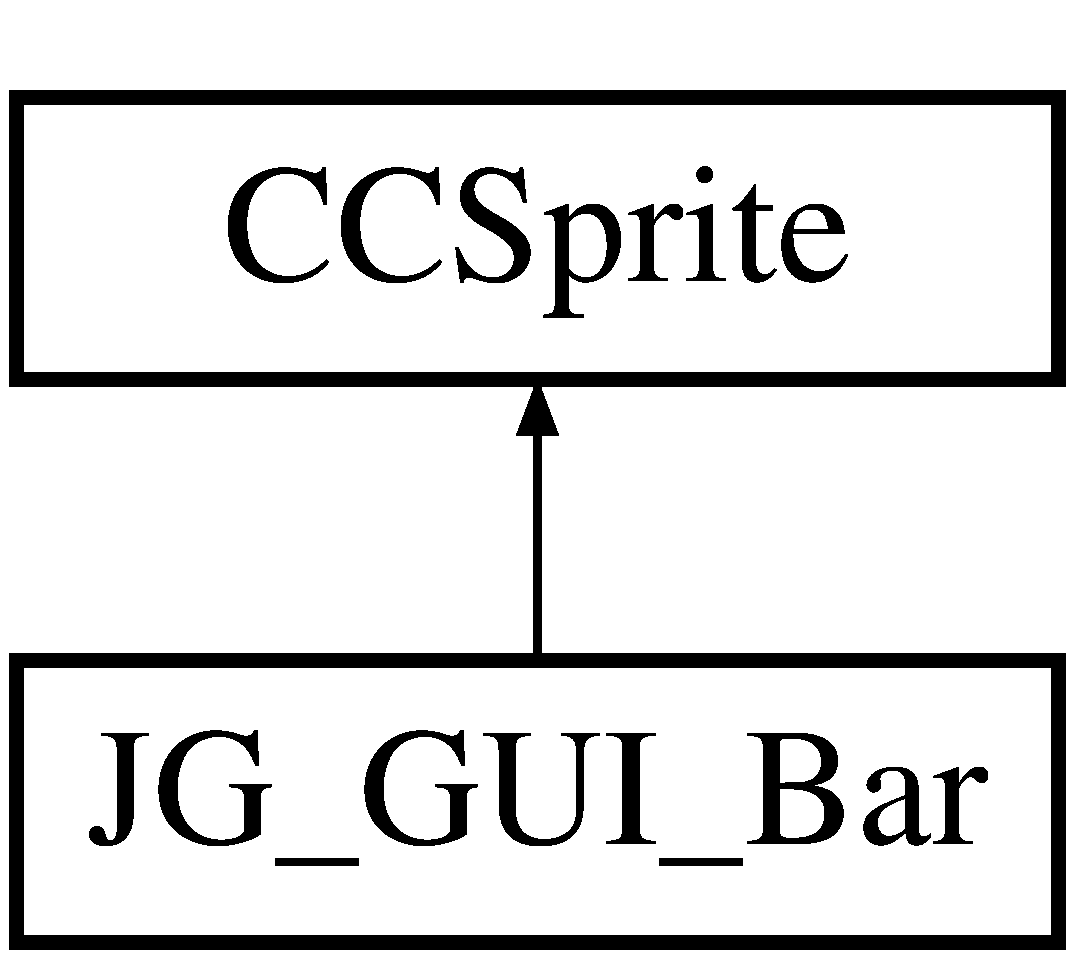
\includegraphics[height=2.000000cm]{class_j_g___g_u_i___bar}
\end{center}
\end{figure}
\subsection*{Public Member Functions}
\begin{DoxyCompactItemize}
\item 
\hypertarget{class_j_g___g_u_i___bar_a1e1defe038b261b82b4fc23b7236956f}{void {\bfseries Init\-Bar} (C\-C\-Point initial\-Position, float new\-Max\-Scale)}\label{class_j_g___g_u_i___bar_a1e1defe038b261b82b4fc23b7236956f}

\item 
\hypertarget{class_j_g___g_u_i___bar_a6e890de091921362483d2526a036a46c}{void {\bfseries Set\-Bar\-Scale} (float scale)}\label{class_j_g___g_u_i___bar_a6e890de091921362483d2526a036a46c}

\end{DoxyCompactItemize}
\subsection*{Static Public Member Functions}
\begin{DoxyCompactItemize}
\item 
\hypertarget{class_j_g___g_u_i___bar_aab9b7d52bf25a3299a8048960b7dd08c}{static \hyperlink{class_j_g___g_u_i___bar}{J\-G\-\_\-\-G\-U\-I\-\_\-\-Bar} $\ast$ {\bfseries Create\-Bar} (C\-C\-Point intial\-Position, float new\-Max\-Scale)}\label{class_j_g___g_u_i___bar_aab9b7d52bf25a3299a8048960b7dd08c}

\end{DoxyCompactItemize}


The documentation for this class was generated from the following files\-:\begin{DoxyCompactItemize}
\item 
J\-G\-\_\-\-G\-U\-I\-\_\-\-Bar.\-h\item 
J\-G\-\_\-\-G\-U\-I\-\_\-\-Bar.\-cpp\end{DoxyCompactItemize}

\hypertarget{class_j_g___hand}{\section{J\-G\-\_\-\-Hand Class Reference}
\label{class_j_g___hand}\index{J\-G\-\_\-\-Hand@{J\-G\-\_\-\-Hand}}
}
Inheritance diagram for J\-G\-\_\-\-Hand\-:\begin{figure}[H]
\begin{center}
\leavevmode
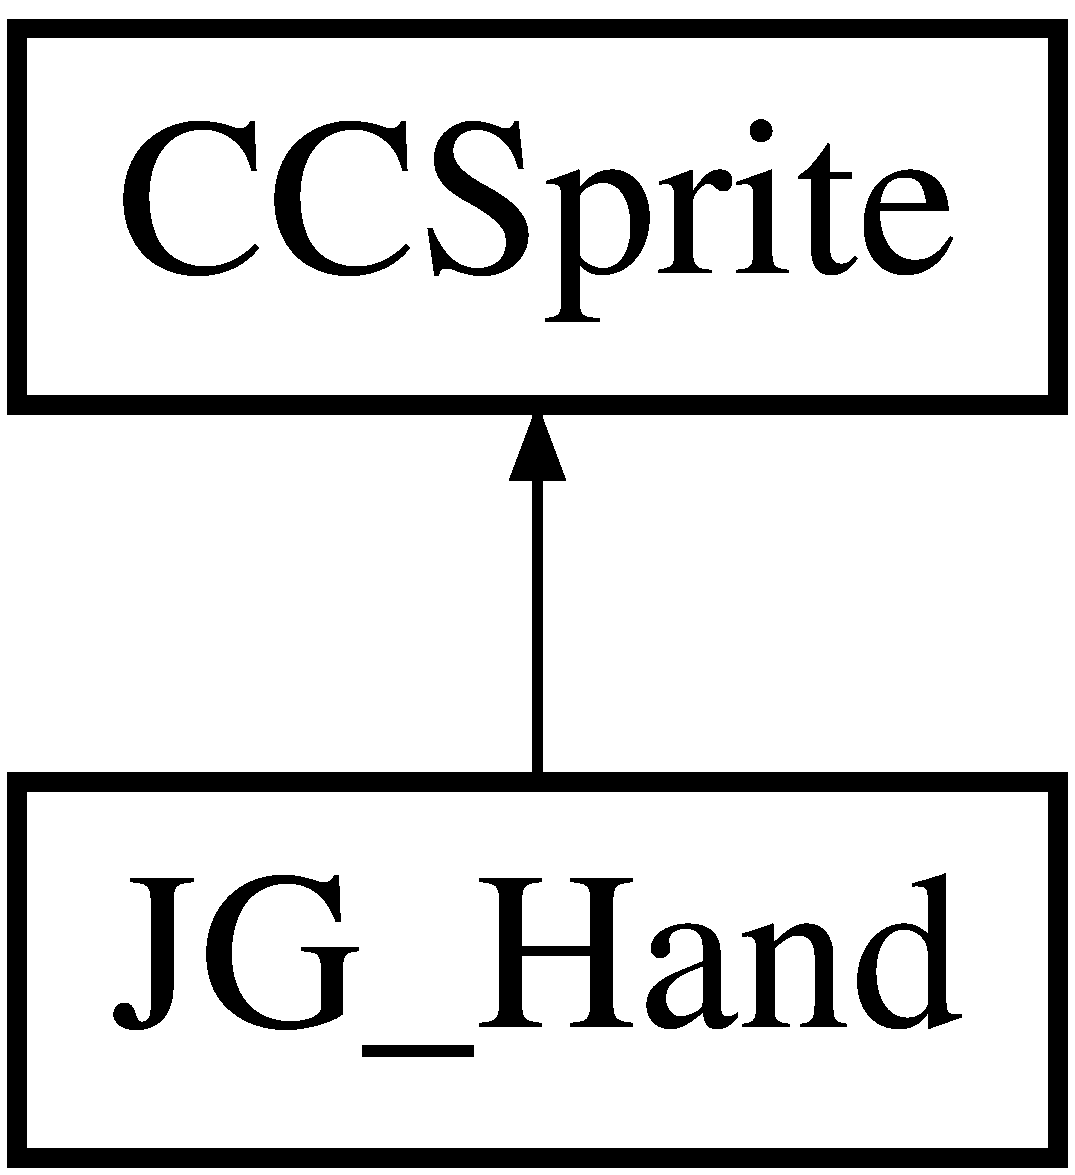
\includegraphics[height=2.000000cm]{class_j_g___hand}
\end{center}
\end{figure}
\subsection*{Public Member Functions}
\begin{DoxyCompactItemize}
\item 
\hypertarget{class_j_g___hand_aa66f82060cc53cf1790d2611476c76c0}{float {\bfseries Get\-Radius} ()}\label{class_j_g___hand_aa66f82060cc53cf1790d2611476c76c0}

\item 
\hypertarget{class_j_g___hand_aca220b8f6b4920e9324dd6b3e4f038ab}{{\bfseries C\-R\-E\-A\-T\-E\-\_\-\-F\-U\-N\-C} (\hyperlink{class_j_g___hand}{J\-G\-\_\-\-Hand})}\label{class_j_g___hand_aca220b8f6b4920e9324dd6b3e4f038ab}

\end{DoxyCompactItemize}
\subsection*{Static Public Member Functions}
\begin{DoxyCompactItemize}
\item 
\hypertarget{class_j_g___hand_af1e8c1afe129641193dc4f459ea3da62}{static \hyperlink{class_j_g___hand}{J\-G\-\_\-\-Hand} $\ast$ {\bfseries create\-With\-File\-Name} (const char $\ast$psz\-File\-Name, C\-C\-Point initial\-Pos)}\label{class_j_g___hand_af1e8c1afe129641193dc4f459ea3da62}

\end{DoxyCompactItemize}
\subsection*{Public Attributes}
\begin{DoxyCompactItemize}
\item 
\hypertarget{class_j_g___hand_abbebb5b5f2b897af0fa566477c817c96}{float {\bfseries radius}}\label{class_j_g___hand_abbebb5b5f2b897af0fa566477c817c96}

\end{DoxyCompactItemize}


The documentation for this class was generated from the following files\-:\begin{DoxyCompactItemize}
\item 
J\-G\-\_\-\-Hand.\-h\item 
J\-G\-\_\-\-Hand.\-cpp\end{DoxyCompactItemize}

\hypertarget{class_j_g___menu___g_u_i}{\section{J\-G\-\_\-\-Menu\-\_\-\-G\-U\-I Class Reference}
\label{class_j_g___menu___g_u_i}\index{J\-G\-\_\-\-Menu\-\_\-\-G\-U\-I@{J\-G\-\_\-\-Menu\-\_\-\-G\-U\-I}}
}
Inheritance diagram for J\-G\-\_\-\-Menu\-\_\-\-G\-U\-I\-:\begin{figure}[H]
\begin{center}
\leavevmode
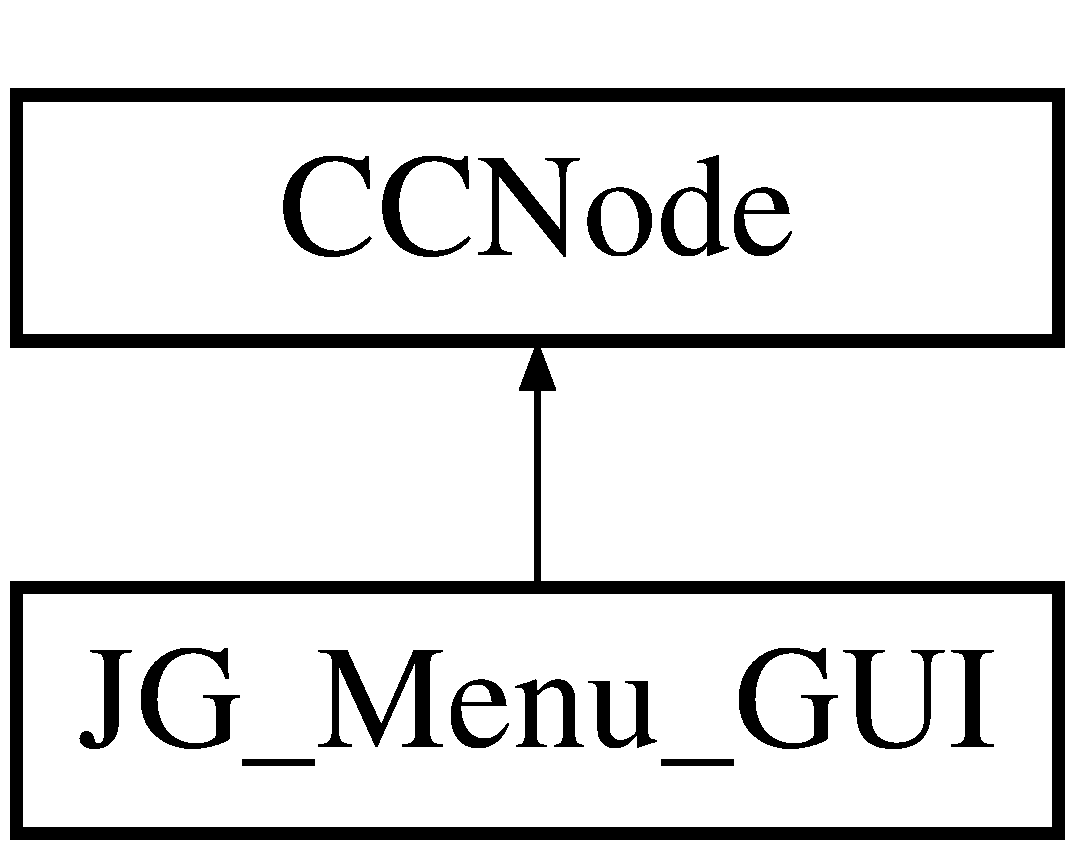
\includegraphics[height=2.000000cm]{class_j_g___menu___g_u_i}
\end{center}
\end{figure}
\subsection*{Static Public Member Functions}
\begin{DoxyCompactItemize}
\item 
\hypertarget{class_j_g___menu___g_u_i_a1af6b38434dcf86b676d7e636422ae24}{static \hyperlink{class_j_g___menu___g_u_i}{J\-G\-\_\-\-Menu\-\_\-\-G\-U\-I} $\ast$ {\bfseries Create\-Menu\-G\-U\-I} (\hyperlink{class_j_g___menu___main}{J\-G\-\_\-\-Menu\-\_\-\-Main} $\ast$menu)}\label{class_j_g___menu___g_u_i_a1af6b38434dcf86b676d7e636422ae24}

\end{DoxyCompactItemize}


The documentation for this class was generated from the following files\-:\begin{DoxyCompactItemize}
\item 
J\-G\-\_\-\-Menu\-\_\-\-G\-U\-I.\-h\item 
J\-G\-\_\-\-Menu\-\_\-\-G\-U\-I.\-cpp\end{DoxyCompactItemize}

\hypertarget{class_j_g___menu___main}{\section{J\-G\-\_\-\-Menu\-\_\-\-Main Class Reference}
\label{class_j_g___menu___main}\index{J\-G\-\_\-\-Menu\-\_\-\-Main@{J\-G\-\_\-\-Menu\-\_\-\-Main}}
}
Inheritance diagram for J\-G\-\_\-\-Menu\-\_\-\-Main\-:\begin{figure}[H]
\begin{center}
\leavevmode
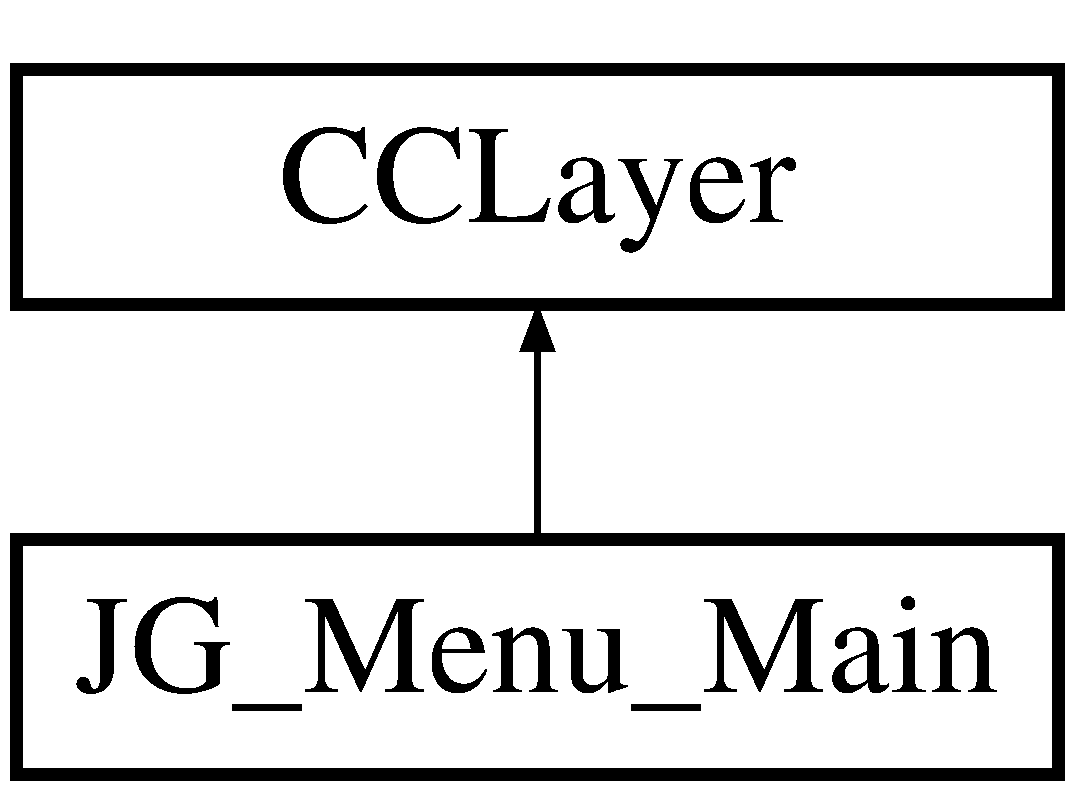
\includegraphics[height=2.000000cm]{class_j_g___menu___main}
\end{center}
\end{figure}
\subsection*{Public Member Functions}
\begin{DoxyCompactItemize}
\item 
\hypertarget{class_j_g___menu___main_ae015e299e7fd365043d747c6198cd418}{virtual bool {\bfseries init} ()}\label{class_j_g___menu___main_ae015e299e7fd365043d747c6198cd418}

\item 
\hypertarget{class_j_g___menu___main_aecbc239ff1644bff785af4e6a72dd516}{void {\bfseries menu\-Close\-Callback} (C\-C\-Object $\ast$p\-Sender)}\label{class_j_g___menu___main_aecbc239ff1644bff785af4e6a72dd516}

\item 
\hypertarget{class_j_g___menu___main_a606ffa5c67ae0d9451922ae2661583c8}{void {\bfseries menu\-Pause\-Call\-Back} (C\-C\-Object $\ast$p\-Sender)}\label{class_j_g___menu___main_a606ffa5c67ae0d9451922ae2661583c8}

\item 
\hypertarget{class_j_g___menu___main_a2abd1c8349ebb5469d4ea533abb69b51}{{\bfseries C\-R\-E\-A\-T\-E\-\_\-\-F\-U\-N\-C} (\hyperlink{class_j_g___menu___main}{J\-G\-\_\-\-Menu\-\_\-\-Main})}\label{class_j_g___menu___main_a2abd1c8349ebb5469d4ea533abb69b51}

\end{DoxyCompactItemize}
\subsection*{Static Public Member Functions}
\begin{DoxyCompactItemize}
\item 
\hypertarget{class_j_g___menu___main_a4725c05fccdb74b94d0b097e6310f743}{static cocos2d\-::\-C\-C\-Scene $\ast$ {\bfseries scene} ()}\label{class_j_g___menu___main_a4725c05fccdb74b94d0b097e6310f743}

\end{DoxyCompactItemize}


The documentation for this class was generated from the following files\-:\begin{DoxyCompactItemize}
\item 
J\-G\-\_\-\-Menu\-\_\-\-Main.\-h\item 
J\-G\-\_\-\-Menu\-\_\-\-Main.\-cpp\end{DoxyCompactItemize}

\hypertarget{class_j_g___path}{\section{J\-G\-\_\-\-Path Class Reference}
\label{class_j_g___path}\index{J\-G\-\_\-\-Path@{J\-G\-\_\-\-Path}}
}
Inheritance diagram for J\-G\-\_\-\-Path\-:\begin{figure}[H]
\begin{center}
\leavevmode
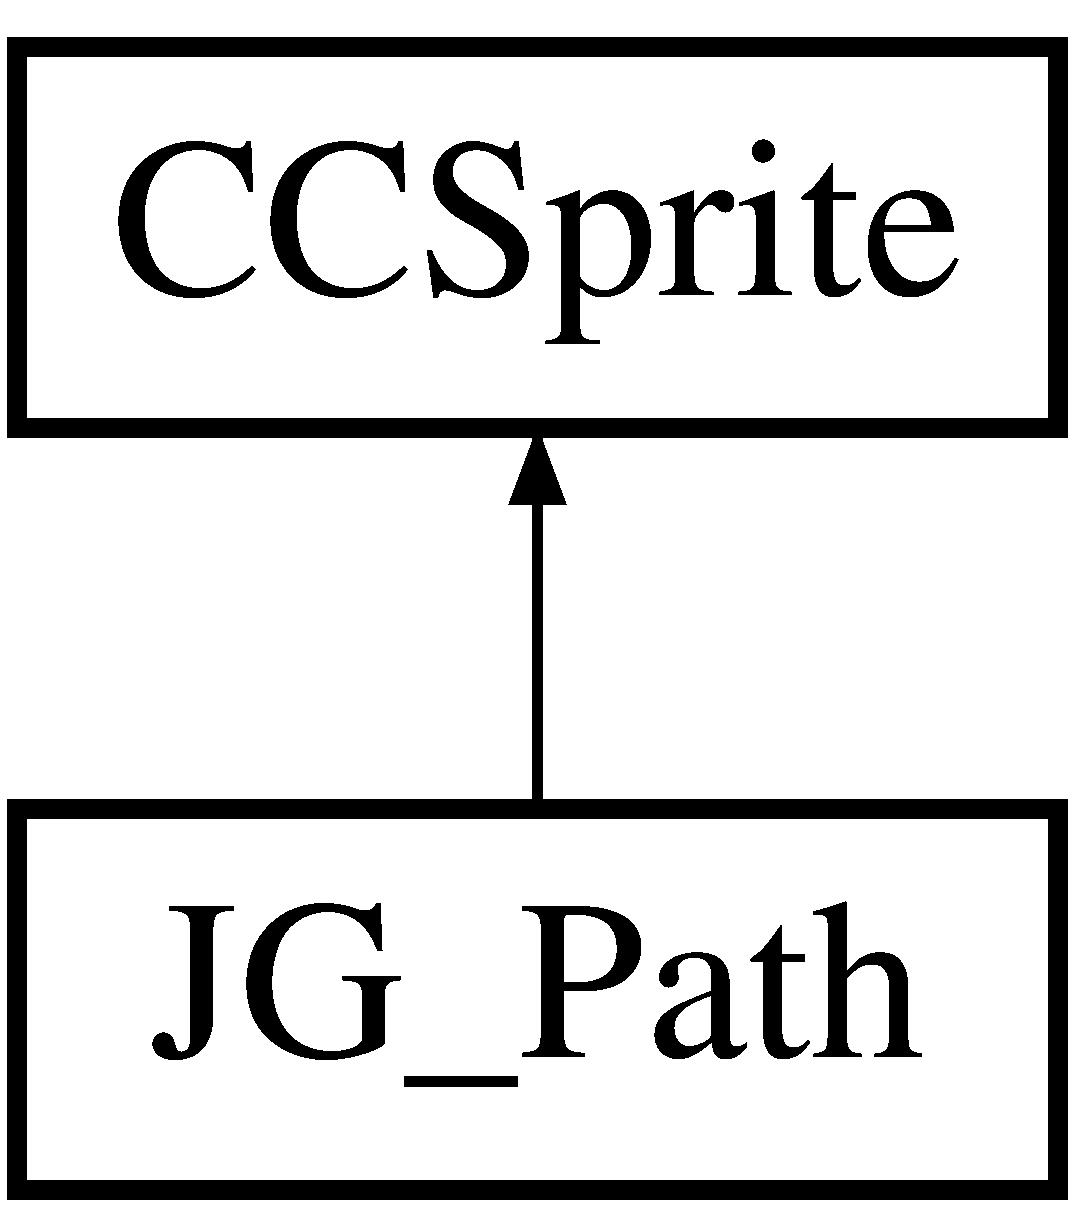
\includegraphics[height=2.000000cm]{class_j_g___path}
\end{center}
\end{figure}
\subsection*{Public Member Functions}
\begin{DoxyCompactItemize}
\item 
\hypertarget{class_j_g___path_ae65379b3c8c17378afb0f7686b150ce9}{void {\bfseries draw} ()}\label{class_j_g___path_ae65379b3c8c17378afb0f7686b150ce9}

\item 
\hypertarget{class_j_g___path_a92dec43ef96e3d4ef52da5bb51c441b2}{void {\bfseries Initial\-Path} (\hyperlink{class_j_g___game___main}{J\-G\-\_\-\-Game\-\_\-\-Main} $\ast$game, float power, C\-C\-Point origin, C\-C\-Point destination)}\label{class_j_g___path_a92dec43ef96e3d4ef52da5bb51c441b2}

\item 
\hypertarget{class_j_g___path_a3f7ab3440f2ec8f3c36ced84e1f8d5fd}{void {\bfseries Set\-Highlight} (bool new\-Highlight)}\label{class_j_g___path_a3f7ab3440f2ec8f3c36ced84e1f8d5fd}

\item 
C\-C\-Point \hyperlink{class_j_g___path_a456741c5da849a3c85b7637ba62d4bff}{Get\-Position\-For\-Length\-Ratio} (float lenght\-Ratio)
\item 
\hypertarget{class_j_g___path_aabf40621781f21d2e6ee48042bb240b8}{void {\bfseries Take\-Damage} (float damage)}\label{class_j_g___path_aabf40621781f21d2e6ee48042bb240b8}

\item 
\hypertarget{class_j_g___path_adeed588e6bd3099d50ef694eba5b7dba}{float {\bfseries Get\-Health} ()}\label{class_j_g___path_adeed588e6bd3099d50ef694eba5b7dba}

\item 
\hypertarget{class_j_g___path_a9e477159ffc3743715b2cb30bd4c29e9}{void {\bfseries Set\-Path\-Enable} (bool enable)}\label{class_j_g___path_a9e477159ffc3743715b2cb30bd4c29e9}

\item 
\hypertarget{class_j_g___path_a99e1856bb8fb5f1b8c2fc1b3d5688610}{bool {\bfseries Is\-Path\-Enabled} ()}\label{class_j_g___path_a99e1856bb8fb5f1b8c2fc1b3d5688610}

\item 
\hypertarget{class_j_g___path_a7f546937079f74890bfc3a28e60756bb}{void {\bfseries Update\-Path\-Health\-State\-Texture} ()}\label{class_j_g___path_a7f546937079f74890bfc3a28e60756bb}

\item 
\hypertarget{class_j_g___path_a89d017af63f4c259656dc58974e8313f}{int {\bfseries Get\-Score} ()}\label{class_j_g___path_a89d017af63f4c259656dc58974e8313f}

\item 
\hypertarget{class_j_g___path_a69f65dc51c5d9b563f9fb583ca709977}{void {\bfseries Reset\-Path} ()}\label{class_j_g___path_a69f65dc51c5d9b563f9fb583ca709977}

\item 
\hypertarget{class_j_g___path_a6b2f029431ab7238028e10613ce77343}{void {\bfseries Set\-Health} (float new\-Health)}\label{class_j_g___path_a6b2f029431ab7238028e10613ce77343}

\end{DoxyCompactItemize}
\subsection*{Static Public Member Functions}
\begin{DoxyCompactItemize}
\item 
\hypertarget{class_j_g___path_a334fac381e5a08f431cc35b2cd65c51d}{static \hyperlink{class_j_g___path}{J\-G\-\_\-\-Path} $\ast$ {\bfseries Create\-Path} (\hyperlink{class_j_g___game___main}{J\-G\-\_\-\-Game\-\_\-\-Main} $\ast$game, float power, C\-C\-Point origin, C\-C\-Point destination)}\label{class_j_g___path_a334fac381e5a08f431cc35b2cd65c51d}

\item 
\hypertarget{class_j_g___path_a6e8e797354d78246e0c4606484ba12be}{static void {\bfseries Initial\-Path\-Health\-States\-For\-Each\-Level} ()}\label{class_j_g___path_a6e8e797354d78246e0c4606484ba12be}

\end{DoxyCompactItemize}
\subsection*{Static Public Attributes}
\begin{DoxyCompactItemize}
\item 
\hypertarget{class_j_g___path_a4e191243a774ac461042854f526af39f}{static std\-::vector\\*
$<$ \hyperlink{struct_path_health_states_for_each_level}{Path\-Health\-States\-For\-Each\-Level} $>$ {\bfseries path\-Health\-States\-For\-Each\-Level}}\label{class_j_g___path_a4e191243a774ac461042854f526af39f}

\end{DoxyCompactItemize}


\subsection{Member Function Documentation}
\hypertarget{class_j_g___path_a456741c5da849a3c85b7637ba62d4bff}{\index{J\-G\-\_\-\-Path@{J\-G\-\_\-\-Path}!Get\-Position\-For\-Length\-Ratio@{Get\-Position\-For\-Length\-Ratio}}
\index{Get\-Position\-For\-Length\-Ratio@{Get\-Position\-For\-Length\-Ratio}!JG_Path@{J\-G\-\_\-\-Path}}
\subsubsection[{Get\-Position\-For\-Length\-Ratio}]{\setlength{\rightskip}{0pt plus 5cm}C\-C\-Point J\-G\-\_\-\-Path\-::\-Get\-Position\-For\-Length\-Ratio (
\begin{DoxyParamCaption}
\item[{float}]{lenght\-Ratio}
\end{DoxyParamCaption}
)}}\label{class_j_g___path_a456741c5da849a3c85b7637ba62d4bff}
returns the position for a ratio of path's length ( i.\-e \-: the position of 0.\-5 length of Path) 

The documentation for this class was generated from the following files\-:\begin{DoxyCompactItemize}
\item 
J\-G\-\_\-\-Path.\-h\item 
J\-G\-\_\-\-Path.\-cpp\end{DoxyCompactItemize}

\hypertarget{class_j_g___score___handler}{\section{J\-G\-\_\-\-Score\-\_\-\-Handler Class Reference}
\label{class_j_g___score___handler}\index{J\-G\-\_\-\-Score\-\_\-\-Handler@{J\-G\-\_\-\-Score\-\_\-\-Handler}}
}
Inheritance diagram for J\-G\-\_\-\-Score\-\_\-\-Handler\-:\begin{figure}[H]
\begin{center}
\leavevmode
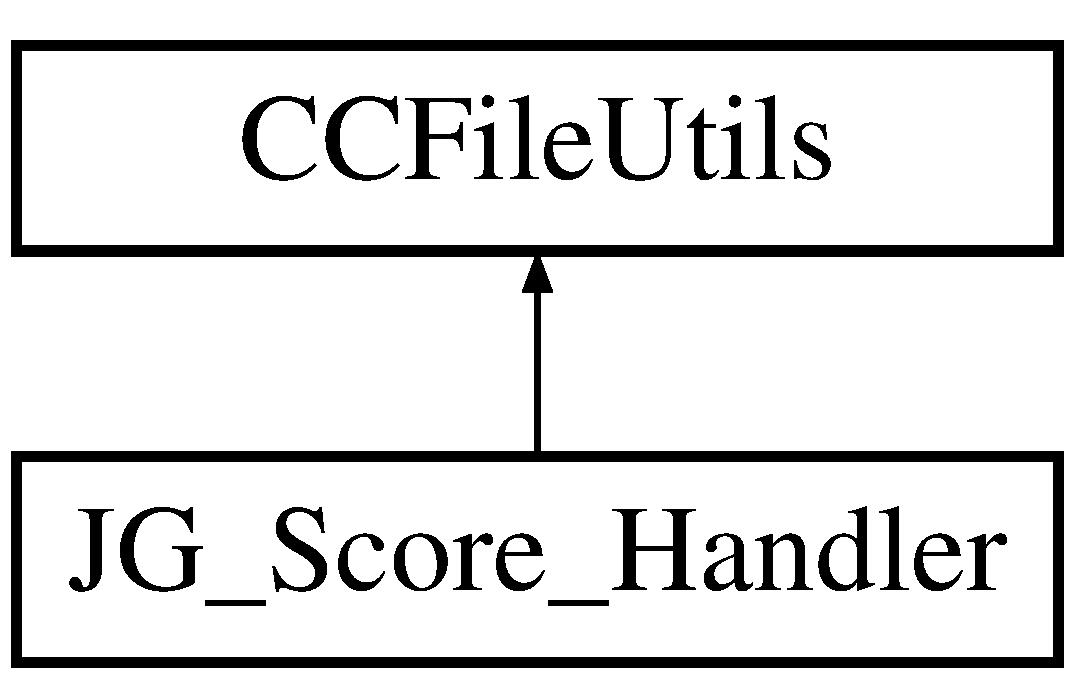
\includegraphics[height=2.000000cm]{class_j_g___score___handler}
\end{center}
\end{figure}
\subsection*{Public Member Functions}
\begin{DoxyCompactItemize}
\item 
\hypertarget{class_j_g___score___handler_aa6036815a089006d0f9885af28797a3a}{void {\bfseries Insert\-Record} (C\-C\-String name, int score, int rank)}\label{class_j_g___score___handler_aa6036815a089006d0f9885af28797a3a}

\item 
\hypertarget{class_j_g___score___handler_a289c33c8e670c2e2b937786d19783078}{vector$<$ \hyperlink{struct_score_table_record}{Score\-Table\-Record} $>$ $\ast$ {\bfseries Get\-High\-Score\-Table} ()}\label{class_j_g___score___handler_a289c33c8e670c2e2b937786d19783078}

\item 
\hypertarget{class_j_g___score___handler_aca1fac35b9e6062738e3d8907f02948e}{\hyperlink{struct_score_table_record}{Score\-Table\-Record} {\bfseries Initializing\-Record} (int rank, string name\-With\-Score)}\label{class_j_g___score___handler_aca1fac35b9e6062738e3d8907f02948e}

\item 
\hypertarget{class_j_g___score___handler_a598968fc031b35762cd3e20b549eb84e}{void {\bfseries Split\-By\-Space} (string input, string \&first\-Part, int \&Second\-Part)}\label{class_j_g___score___handler_a598968fc031b35762cd3e20b549eb84e}

\end{DoxyCompactItemize}


The documentation for this class was generated from the following files\-:\begin{DoxyCompactItemize}
\item 
J\-G\-\_\-\-Score\-\_\-\-Handler.\-h\item 
J\-G\-\_\-\-Score\-\_\-\-Handler.\-cpp\end{DoxyCompactItemize}

\hypertarget{class_j_g___score_popup}{\section{J\-G\-\_\-\-Score\-Popup Class Reference}
\label{class_j_g___score_popup}\index{J\-G\-\_\-\-Score\-Popup@{J\-G\-\_\-\-Score\-Popup}}
}
Inheritance diagram for J\-G\-\_\-\-Score\-Popup\-:\begin{figure}[H]
\begin{center}
\leavevmode
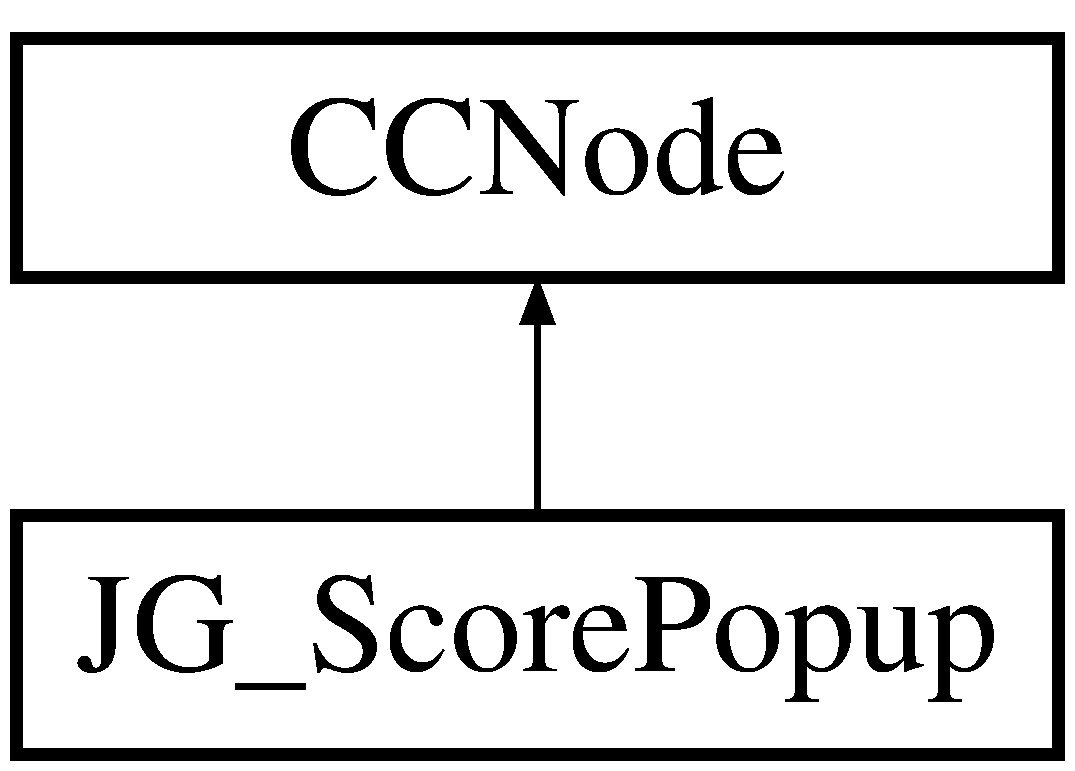
\includegraphics[height=2.000000cm]{class_j_g___score_popup}
\end{center}
\end{figure}
\subsection*{Static Public Member Functions}
\begin{DoxyCompactItemize}
\item 
\hypertarget{class_j_g___score_popup_ac083664691cd0f959bd50cfee59b1867}{static \hyperlink{class_j_g___score_popup}{J\-G\-\_\-\-Score\-Popup} $\ast$ {\bfseries Create\-Score\-Popup} (\hyperlink{class_j_g___game___main}{J\-G\-\_\-\-Game\-\_\-\-Main} $\ast$game, int score, int multiplier, C\-C\-Point position)}\label{class_j_g___score_popup_ac083664691cd0f959bd50cfee59b1867}

\end{DoxyCompactItemize}


The documentation for this class was generated from the following files\-:\begin{DoxyCompactItemize}
\item 
J\-G\-\_\-\-Score\-Popup.\-h\item 
J\-G\-\_\-\-Score\-Popup.\-cpp\end{DoxyCompactItemize}

\hypertarget{struct_path_health_states_for_each_level}{\section{Path\-Health\-States\-For\-Each\-Level Struct Reference}
\label{struct_path_health_states_for_each_level}\index{Path\-Health\-States\-For\-Each\-Level@{Path\-Health\-States\-For\-Each\-Level}}
}
\subsection*{Public Attributes}
\begin{DoxyCompactItemize}
\item 
\hypertarget{struct_path_health_states_for_each_level_a174c4a14b31fa638a721944d5e2db7d9}{std\-::vector$<$ C\-C\-Texture2\-D $\ast$ $>$ {\bfseries health\-State\-Textures}}\label{struct_path_health_states_for_each_level_a174c4a14b31fa638a721944d5e2db7d9}

\end{DoxyCompactItemize}


The documentation for this struct was generated from the following file\-:\begin{DoxyCompactItemize}
\item 
J\-G\-\_\-\-Path.\-h\end{DoxyCompactItemize}

\hypertarget{struct_score_table_record}{\section{Score\-Table\-Record Struct Reference}
\label{struct_score_table_record}\index{Score\-Table\-Record@{Score\-Table\-Record}}
}
\subsection*{Public Attributes}
\begin{DoxyCompactItemize}
\item 
\hypertarget{struct_score_table_record_a55b55dde6a43ce872aaa1cca88528c35}{string {\bfseries name}}\label{struct_score_table_record_a55b55dde6a43ce872aaa1cca88528c35}

\item 
\hypertarget{struct_score_table_record_a8cf8a756ffefaf10e38fa8a6e430e270}{int {\bfseries score}}\label{struct_score_table_record_a8cf8a756ffefaf10e38fa8a6e430e270}

\item 
\hypertarget{struct_score_table_record_ae1a14feca0c0ed9bbc8913f38abc634d}{int {\bfseries rank}}\label{struct_score_table_record_ae1a14feca0c0ed9bbc8913f38abc634d}

\end{DoxyCompactItemize}


The documentation for this struct was generated from the following file\-:\begin{DoxyCompactItemize}
\item 
J\-G\-\_\-\-Score\-\_\-\-Handler.\-h\end{DoxyCompactItemize}

\hypertarget{struct_s_enemy_types}{\section{S\-Enemy\-Types Struct Reference}
\label{struct_s_enemy_types}\index{S\-Enemy\-Types@{S\-Enemy\-Types}}
}
\subsection*{Public Attributes}
\begin{DoxyCompactItemize}
\item 
\hypertarget{struct_s_enemy_types_ad8e14661ad8fa467a36f4a0946c0b9b2}{\hyperlink{class_j_g___factory___base}{J\-G\-\_\-\-Factory\-\_\-\-Base} $\ast$ {\bfseries factory}}\label{struct_s_enemy_types_ad8e14661ad8fa467a36f4a0946c0b9b2}

\item 
\hypertarget{struct_s_enemy_types_a44664a0343349fd70e9668d1f25da3af}{int {\bfseries current\-Chance}}\label{struct_s_enemy_types_a44664a0343349fd70e9668d1f25da3af}

\item 
\hypertarget{struct_s_enemy_types_a3f0dbd0095863f5c07389eef2f48eb5e}{int {\bfseries chance\-Increase\-Per\-Round}}\label{struct_s_enemy_types_a3f0dbd0095863f5c07389eef2f48eb5e}

\end{DoxyCompactItemize}


The documentation for this struct was generated from the following file\-:\begin{DoxyCompactItemize}
\item 
J\-G\-\_\-\-Attack\-Wave\-\_\-\-Base.\-h\end{DoxyCompactItemize}

\hypertarget{struct_s_touch_info}{\section{S\-Touch\-Info Struct Reference}
\label{struct_s_touch_info}\index{S\-Touch\-Info@{S\-Touch\-Info}}
}
\subsection*{Public Attributes}
\begin{DoxyCompactItemize}
\item 
\hypertarget{struct_s_touch_info_a476c6db5c7f5ee0987fef6221fbceaf7}{C\-C\-Touch $\ast$ {\bfseries touch}}\label{struct_s_touch_info_a476c6db5c7f5ee0987fef6221fbceaf7}

\item 
\hypertarget{struct_s_touch_info_a354b68630606341541b282561bb4c292}{\hyperlink{class_j_g___hand}{J\-G\-\_\-\-Hand} $\ast$ {\bfseries hand}}\label{struct_s_touch_info_a354b68630606341541b282561bb4c292}

\item 
\hypertarget{struct_s_touch_info_aaed3c79798657884c11efa8a0e1fcb3f}{\hyperlink{class_j_g___ball}{J\-G\-\_\-\-Ball} $\ast$ {\bfseries ball}}\label{struct_s_touch_info_aaed3c79798657884c11efa8a0e1fcb3f}

\item 
\hypertarget{struct_s_touch_info_ab444619d360b1742837805506f9e1779}{bool {\bfseries b\-Is\-Dir\-Valid}}\label{struct_s_touch_info_ab444619d360b1742837805506f9e1779}

\item 
\hypertarget{struct_s_touch_info_a76f5cc268d81a4d3c80884669c7cc050}{float {\bfseries remaining\-Time}}\label{struct_s_touch_info_a76f5cc268d81a4d3c80884669c7cc050}

\item 
\hypertarget{struct_s_touch_info_ae1dd747adb4a406c03f18b5ffa45df6a}{C\-C\-Point {\bfseries initial\-Time\-Position}}\label{struct_s_touch_info_ae1dd747adb4a406c03f18b5ffa45df6a}

\end{DoxyCompactItemize}


The documentation for this struct was generated from the following file\-:\begin{DoxyCompactItemize}
\item 
J\-G\-\_\-\-Game\-\_\-\-Main.\-h\end{DoxyCompactItemize}

\hypertarget{structtag_resource}{\section{tag\-Resource Struct Reference}
\label{structtag_resource}\index{tag\-Resource@{tag\-Resource}}
}


The cocos2d Application.  




{\ttfamily \#include $<$App\-Delegate.\-h$>$}

\subsection*{Public Attributes}
\begin{DoxyCompactItemize}
\item 
\hypertarget{structtag_resource_a8640b003a8c5eef990ac1d0bd092c1c9}{cocos2d\-::\-C\-C\-Size {\bfseries size}}\label{structtag_resource_a8640b003a8c5eef990ac1d0bd092c1c9}

\item 
\hypertarget{structtag_resource_a347655ec02bf050e771cb4e6cb595537}{char {\bfseries directory} \mbox{[}100\mbox{]}}\label{structtag_resource_a347655ec02bf050e771cb4e6cb595537}

\end{DoxyCompactItemize}


\subsection{Detailed Description}
The cocos2d Application. 

The reason for implement as private inheritance is to hide some interface call by C\-C\-Director. 

The documentation for this struct was generated from the following file\-:\begin{DoxyCompactItemize}
\item 
App\-Delegate.\-h\end{DoxyCompactItemize}

%--- End generated contents ---

% Index
\newpage
\phantomsection
\addcontentsline{toc}{part}{Index}
\printindex

\end{document}
